% set margins and font
\documentclass[12pt,letterpaper]{article}
\usepackage[margin=1in]{geometry}
\usepackage{helvet}
\renewcommand{\familydefault}{\sfdefault}

% amsmath and amssymb packages, useful for mathematical formulas and symbols
\usepackage{amsmath,amssymb}

% citation manager
\usepackage[english]{babel}
 
\usepackage[square,numbers]{natbib}
\bibliographystyle{abbrvnat}

% include images
\usepackage{graphicx}
\usepackage[font=footnotesize,labelfont=bf]{caption} % reduce default caption font size

% Use Unicode characters when possible
\usepackage[utf8x]{inputenc}

% array package and thick rules for tables
\usepackage{array}

% Remove comment for double spacing
\usepackage{setspace} 
%\doublespacing
\linespread{2}

% text symbol package
\usepackage{textcomp}

\begin{document}
\vspace*{0.2in}

% begin roman numeral page numbering
\pagenumbering{roman}

% TITLE PAGE
\begin{titlepage}
	\centering
	\vspace{1cm}
	{\scshape \large The Structure of Behavioral Variation Within a Genotype\par}
	\vspace{1.0cm}
	A dissertation presented\par \vspace{0.35cm}
	by\par \vspace{0.35cm}
	Zachary Werkhoven\par \vspace{0.35cm}
	to\par \vspace{0.35cm}
	The Department of Molecular and Cellular Biology\par \vspace{0.35cm}
	in partial fulfillment of the requirements\par \vspace{0.35cm}
	for the degree of\par \vspace{0.35cm}
	Doctor of Philosophy\par \vspace{0.35cm}
	in the subject of\par \vspace{0.35cm}
	Molecular and Cellular Biology\par \vspace{0.35cm}
	\vfill
	Harvard University\par
	Cambridge, Massachusetts\par
	August 2019
	\vfill
\end{titlepage}
\clearpage

% COPYRIGHT PAGE
\topskip0pt
\vspace*{\fill}
    \begin{center}
    \textcopyright \hspace{0.01in} 2019 Zachary Werkhoven
    \end{center}
    \begin{center}
    All Rights Reserved.
    \end{center}
    \thispagestyle{empty}       % set page numbering style to blank
\vspace*{\fill}
\clearpage

% ABSTRACT
\setcounter{page}{3}
\begin{abstract}
    aasdfj addsa sd ds das s adfsd adsf aasdfj addsa sd ds das s adfsd adsf aasdfj addsa sd ds das s adfsd adsf aasdfj addsa sd ds das s adfsd adsf aasdfj addsa sd ds das s adfsd adsf aasdfj addsa sd ds das s adfsd adsf aasdfj addsa sd ds das s adfsd adsf aasdfj addsa sd ds das s adfsd adsf aasdfj addsa sd ds das s adfsd adsf aasdfj addsa sd ds das s adfsd adsf aasdfj addsa sd ds das s adfsd adsf aasdfj addsa sd ds das s adfsd adsf aasdfj addsa sd ds das s adfsd adsf aasdfj addsa sd ds das s adfsd adsf aasdfj addsa sd ds das s adfsd adsf aasdfj addsa sd ds das s adfsd adsf aasdfj addsa sd ds das s adfsd adsf aasdfj addsa sd ds das s adfsd adsf aasdfj addsa sd ds das s adfsd adsf aasdfj addsa sd ds das s adfsd adsf aasdfj addsa sd ds das s adfsd adsf aasdfj addsa sd ds das s adfsd adsf  
\end{abstract}

% insert chapter title page
\clearpage
\begin{center}
    \Large\section{Chapter 1}
    \pagenumbering{arabic}      % switch page numbering to arabic numerals
    \setcounter{page}{1}        % reset the page counter to 1
    \thispagestyle{empty}       % set page numbering style to blank
    \clearpage
\end{center}

\subsection{Introduction}

Individuals display idiosyncratic differences in behavior that often persist through time and are robust to situational context. Some persistent individual behavioral traits commonly occur in correlated groups and can therefore be said to covary together. Observations covarying behavioral traits have been limited in scope and thus the sources and extent of behavioral covariation is not well-understood. Behavioral covariation occurs any time behavioral traits are linked and can be detected as a correlation between two or more behaviors. For example, navigation with respect to light (phototaxis) and navigation with respect to temperature (thermotaxis) covary, then individuals that are positively phototactic are more likely to be positively thermotactic and vice versa. 

Behavioral ethologists have long understood that ”types” of human and animal personalities can be described as groups correlated that occur together. Propensities for human social behaviors such assertiveness, talkativeness, and impulsiveness are commonly thought to occur together and described as extraversion, while passivity, shyness, and deliberateness are described as introversion. Although the total space of human social behaviors is very high dimensional, extraversion-introversion is thought to constitute a fundamental dimension in human social behavior, thereby reducing the effective dimensionality of the space of social behaviors. Behavioral symptoms also frequently correlate when neuronal function is perturbed in human mental disorders. Severity of stereotyped motor behaviors and language impairments correlate in autism spectrum disorder, and sleep correlates with repetitive behaviors in bipolar disorder. In animal species, correlated suites of behaviors are known as behavioral syndromes. Aggressive behaviors such fighting over mates or food are correlated with exploratory behaviors such as foraging and social interaction in diverse species of insects, arachnids, fish, and birds. These behaviors are frequently described as falling on an axis of boldness-shyness. 

The prevalence of behavioral correlation suggests that covariation is likely a broad feature of behavior, but the extent to which behaviors covary, how behavioral covariation arises, and whether or not behavioral variation has a characteristic structure is not well-understood. Profiling behavioral variability therefore has the potential to answer important questions in biology: Is effective dimensionality of behavioral high or low? What does the structure of behavioral variability look like across individuals and across genotypes? Is the correlational structure of behavior stereotyped or variable? Can behavioral correlations be linked to neural circuit structure or gene expression?

\subsection{Drosophila as a Model of Individual Behavioral Variation}

Organisms such as insects with significantly less complex brains than humans (approximately 6 orders of magnitude fewer neurons) display a diverse array of behaviors that vary by genotype and environment. Fruit flies are an attractive model for studying behavioral variation. In addition to the ease of maintaining many thousands of individuals and wealth of genetic tools available in fruit flies, they respond to a variety of visual, olfactory, thermal and mechanical cues. Moreover, fruit flies show considerable behavioral variation across mutant and wild-type genotypes.

Assaying individual behavioral variability poses many practical challenges. Capturing the effective dimensionality of individual variation requires profiling individual behaviors very broadly. Measuring behavioral covariability broadly comes at the cost increased number of comparisons as the number of pair-wise combinations of measures grows at a factorial rate ${n \choose 2}$. Even with a relatively small number of behavioral measurements (e.g. tens of measures), high statistical power is required to deal with problems of multiple comparisons. Small body size, short generation time, and high fecundity make flies well-suited to assaying individual behaviors at high throughput. Thus drosophila has emerged as a model for individual behavioral variation. 

Fruit flies also display individual variability in locomotor handedness that persists well into adulthood. Fly handedness can be measured in flies by placing them in Y-shaped arenas scoring their trajectories as right or left-handed as they pass through the center of the arena, choosing either the right or left arm. Hundreds of flies can be assayed simultaneously this way making hundreds of choices each, providing robust measurements of individual with high statistical confidence. When assayed this way, individuals display significant individual variation (e.g. some flies display extreme right turn probabilities of 0.9 and 0.1). Similarly high-throughput assays have been used to measure individual variation in phototactic and thermotactic preferences. In all behaviors measured, individual flies showed individual variability well beyond what would be expected if individual choices were drawn randomly from a shared distribution (i.e. if all individuals make choices with the same probability). These findings demonstrate the feasibility of drosphila as a model system for assaying individual behavioral variability and show that flies display individual variability in behaviors with and without apparent ethological consequence. 

\subsection{Neural Circuit Bottlenecks as a Potential Source of Behavioral Covariation}

Isogenic D. melanogaster raised in the same environment show idiosyncratic variations in many
behaviors across sensory modalities that are stable throughout an individual’s life 6-8. Interestingly, inbred flies show individual behavioral variability in locomotor handedness. Counter-intuitively, variability in this context increases as genetic diversity decreases. Crossing flies from the distribution tails of locomotor handedness together (i.e. extreme "righties" crossed to each other and extreme "lefties" crossed to each other). Collectively these results suggest a role for non-genetic, non-heritable sources of individual behavioral variability.

While there are well-characterized and understood examples of genetic and developmental constraints on trait covariation, evidence of behavioral covariation while genes and environment are held constant suggests that neural architecture is a likely developmental source of behavioral constraint. Behavioral circuits that depend on overlapping sets of neurons may vary together in ways that reflect variations in those neurons. For example, flies with a higher or lower ratio of inhibitory to excitatory synapses in the descending motor neurons of their rear legs could plausibly show correlations in many posterior limb behaviors such as wing and abdomen grooming. If such circuit bottlenecks induce behavioral covariation, principal behavioral dimensions may be mappable to locations in the nervous system. Motor neurons are an obvious site of convergence in behavioral circuits, but more elusive sites of convergence may exist in the web of connections that underlie sensorimotor transformations such as the central brain.

Neural circuit constraints are one interesting possible source of behavioral covariation and one that may help explain how variation arises in the absence of genetic diversity but remain a largely unexplored source of constraint on behavior due to practical considerations associated with measuring it independently of genetic and environmental sources. Isogenic and environmentally matched fruit flies offer a system to study individual differences in neural circuitry as a source of behavioral variation. In particular, large behavioral screens that can holistically profile behavior may help identify clusters of behaviors that correlation across individuals. When combined with sparse genetic driver lines thermogenetic and optogenetic tools for neural activation and silencing provide a method to systematically perturb small components of neural circuits. Combining behavioral screens with neural circuit manipulations offers two possible benefits: 1) the potential to independently validate clustered behaviors by inducing correlated shifts in behavior through circuit manipulation and 2) localization of behavioral correlations to specific neurons or brain regions. Probing neural circuit constraints on behavior is a necessary step in elucidating the interplay between genes and the underlying neural structure in both evolution and disease, and may suggest a mechanisms for pleiotropic effects on behaviors.

\subsection{Holistic Behavioral Profiling}

The above example of phototaxis and thermotaxis are behaviors one might expect to correlate because sources of light such as the sun are also sources of heat. Although it seems probable that many clusters of correlated behaviors may belong to groups behaviors of shared ethological and physical relevance, correlated behaviors need not have any intuitive relationship. Known correlated groups of behaviors such as boldness-shyness were discovered because specific hypothesis about related behaviors led to studies that were designed to specifically assay those behaviors, but one compelling reason to profile behavioral as holistically as possible is to reveal surprising behavioral clusters that may point to interesting features of the behaviors themselves or an expected and shared biological underpinning. Probing the structure of behavioral variability more generally requires measuring as many behaviors as possible to capture the totality of behavioral variation as completely as possible.

Profiling individual as deeply as possible across a broad range of contexts has become a recent goal of behavioral ethologists. Unsurprisingly, animal behaviors are very diverse and capturing their entire behavioral repertoire presents substantial challenges such as: how to define behaviors, how to feasibly measure multiple behaviors in the same animal, how to measure behaviors that are broadly representative of an animal's total behavior, and how to achieve high enough sampling.

Historically, behavioral measurements have been scored by hand. The limited throughput of manual scoring forced a trade off between depth of and breadth of measurements, resulting in two generically broad approaches to profiling behaviors. The first approach typically focuses on small numbers of individuals where their behaviors are scored on a trial by trial basis for each individual separately and are therefore typically low throughput. The ability to focus on single trials sequentially allows for complex behavioral tasks with potential for minute discrimination between responses which may be composed of multiple features (though the approach also accommodates simple paradigms as well). Examples of this approach include psycho-physical measurements in humans and animals or manual scoring of social interaction between individuals. The second approach, focuses on collective measurement of the responses of groups and is therefore potentially high-throughput. The need to score behavior in groups destroys information about individual responses and also commonly requires thresholding or binning responses. Examples of this approach include classic assays of phototaxis and geotaxis in fruit flies where population responses are measured as the fraction of animals falling inside a number vertically marked zones after being tapped to the bottom of a tube.

More recently, omics based approaches to behavioral measurement have been applied to the study of behavior with success. The Drosophila Genomics Reference Panel (DGRP) is one example of such an approach. The DGRP is a collection of approximately 200 \textit{Drosophila melanogaster} lines of inbred from the wild population of flies in Raleigh, North Carolina. The DGRP serves as snapshot of the genetic diversity present in a wild population of flies and a common reference point between studies. This common reference point has enabled the construction of a database of behavioral phenotypes measured on the DGRP across more than a dozen studies. Behaviors assayed on the DGRP are largely measured at the population-level and do not contain information about individual behaviors. Nonetheless, the DGRP phenotype collection offers a unique opportunity to study the structure of behavior across natural genotypic variation and includes measures of behaviors such as phototaxis, geotaxis, olfaction, and sleep.

Machine learning can be applied to automated measurements of behavior for representations of behavior that are both nuanced and broad in scope. The Janelia Automated Animal Behavior Annotator (JAABA) uses supervised machine learning to classify animal behaviors from video data. Tracking data extracted from videos such as the position and orientation of animals and their body parts is used to engineer a variety of features that contain information about their behavior changes over time. Users then define a set of behaviors to classify and provide examples of each. Classifiers are trained examples and then used to detect new instances of the behaviors in videos that the classifiers have never seen. The rich set of features fed into the algorithm contains detailed information about the posture and movement of the animals that enables the classifiers to detect minute details of behavior that might be difficult for a human to detect. 

JAABA is of particular interest because it has been used extensively to classify behavior of individual fruit flies. Robie et al. used JAABA to screen the effects of neural circuit manipulation across a diverse set of neural driver lines. In total, they profiled the behavior of 2,204 Gal4 lines driving expression a temperature-sensitive cation channel, dTrpA1. JAABA was used to classify 14 behaviors on short videos captured of groups of flies at the restrictive temperature. Although measurements were performed on individuals, the individual component of variability cannot be decoupled from inter-individual internal state variation the short duration of the videos and lack of repeated measurements of the individuals. The study represents a wealth of behavioral variability in response to neural circuit perturbation.

Unlike supervised learning methods which require behaviors to be defined before classification, unsupervised classification of behavior can be used to assign labels to behaviors without any a priori definition. Unsupervised classification has recently used to characterize fruit fly behavior via the motion-mapper pipeline developed by Berman et al. The motion-mapper pipeline relies on the assumption that animal behaviors consist of stereotyped, spatio-temporal postural sequences to generate distinct behavioral labels. The pipeline assays spontaneous exploratory behavior via videos of single flies recorded at high spatial and temporal resolution. Pixels from images are decomposed into high-dimensional representation of the animal's postural dynamics. Ultimately, frames in the high-dimensional representation are clustered in a low-dimensional representation via the t-SNE algorithm and assigned a classification based on those clusters. Unsupervised classification is particularly promising for holistic profiling of individual behavioral because 1) it attempts represent the total observed behavioral space by assigning a label to all frames and 2) it requires no assumption about the number of distinct classifications.

The motion-mapper pipeline has been applied to natural behavioral variation and the effects of neural circuit perturbations on behavior. Male and female behavioral embeddings showed sexually dimorphic structure in \textit{D. melanogaster}, with increased occupancy of locomotor behaviors and decreased occupancy of resting and slow moving behaviors in female flies. Flies showed significantly less intra-individual than inter-individual variation within a wild-type genotype, consistent with persistent individual behavioral differences. Cande and colleagues used motion-mapper to characterize the effects of descending activation through optogenetic manipulation. Activation of single descending neuron types frequently produced stereotyped changes in behavior, in many cases resulting in changes primarily to a single region of the behavioral map (e.g. posterior limb movements).

\subsection{Evolution of Correlated Behaviors and the G-Matrix}

Do behaviors evolve independently or as sets of behavior? 
The introduction of covariation in behavior lowers the effective dimensionality of behaviors that animals can exhibit. This raises the possibility that covariation may constrain the space of evolutionary space that behaviors can explore, causing some behaviors to evolve as sets of behaviors. This possibility is analogous to the phenomenon of pleiotropy where a single gene influences more than one phenotype, which has been hypothesized to have a stabilizing effect on evolution. Evolutionary geneticists typically think of correlated traits as being coupled by mutual dependence on common genes, developmental origins, or environmental factors. Regardless of the source, the quantitative study of covariation of traits and their effect of evolutionary trajectories has been formalized in the G-matrix (i.e. the matrix of additive genetic variance and covariances). 

There are two basic questions of interest to behavioral ethologists and evolutionary biologists: 1) Which behaviors are correlated or anti correlated? 2) Is the correlational structure of behaviors stable or unstable? Understanding which behaviors are correlated and how consistently groups of behaviors


% insert chapter title on its own page
\clearpage
\begin{center}
    \Large\textbf{Chapter 2}
    \thispagestyle{empty}       % set page numbering style to blank
    \clearpage
\end{center}

\section*{MARGO: a Platform for High-Throughput Individual Ethology}

% Please keep the abstract below 300 words
\section*{Abstract}

Fast object tracking in real time allows convenient tracking of very large numbers of animals and closed-loop experiments that control stimuli for multiple animals in parallel. We developed MARGO, a real-time animal tracking suite for custom behavioral experiments. We demonstrated that MARGO can rapidly and accurately track large numbers of animals in parallel over very long timescales. We incorporated control of peripheral hardware, and implemented a flexible software architecture for defining new experimental routines. These features enable closed-loop delivery of stimuli to many individuals simultaneously. We highlight MARGO's ability to coordinate tracking and hardware control with two custom behavioral assays (measuring phototaxis and optomotor response) and one optogenetic operant conditioning assay. There are currently several open source animal trackers. MARGO’s strengths are 1) robustness, 2) high throughput, 3) flexible control of hardware and 4) real-time closed-loop control of sensory and optogenetic stimuli, all of which are optimized for large-scale experimentation.

\linenumbers

% Use "Eq" instead of "Equation" for equation citations.
\section*{Introduction}

The recent introduction of automated methods for measuring behaviors offers a level of throughput that has gradually reduced the need to trade between depth and breadth of behavioral measurements. Cheap electronic components such as infrared beam break detectors enabled course detection of animal position. The TriKinetics Drosophila Activity Monitor (DAM) estimates animal activity level by counting the number crosses over a beam break sensor. A similar strategy has also been used to measure phototactic behavior in a T-maze by positioning sensors in arms on either side of the choice point. More recently, the availability of inexpensive, high-resolution cameras has enabled widespread use of video data in animal behavioral measurement. Automated tracking of animal centroids and body segments have revolutionized the study of behavior by enabling precise measurement of the location and posture of animals. When coupled with other animals or automated stimulus delivery, animal tracking provides detailed descriptions of behavioral dynamics in response social and stimulus driven contexts. 

Automated animal tracking methods have become commonplace in the study of behavior. They enable large sample sizes, high statistical power, and more rapid inference of mechanisms giving rise to behavior. Existing animal trackers vary in computational complexity and are often specialized for particular imaging configurations or behavioral measurements. Trackers can assist in a wide range of experimental tasks such as monitoring activity, measuring response to stimuli \cite{Fry_TrackFly_2008,Donelson_High_2012}, and locating body parts over time \cite{Mathis_DeepLabCut_2018,Pereira_Fast_2018}. Some trackers are designed to track and maintain identities of multiple individuals occupying the same arena \cite{Prez-Escudero_idTracker_2014,Eyjolfsdottir_Detecting_2014,Rodriguez_ToxId_2017,romero-ferrero_2019} while others measure the collective activity of groups without maintaining identities or rely on physical segregation of animals to ensure trajectories never collide \cite{Ramot_The_2008,Swierczek_High_2011,Itskovits_A_2017,Scaplen_Automated_2019}. But few of these trackers are designed as platforms for high throughput, hardware control, and flexible experimental reconfiguration. 

Improvements in machine learning and template matching approaches to object localization and classification have made it possible to efficiently train models that accurately track and classify a variety of animal species and visually distinguish identities of individuals across time \cite{Eyjolfsdottir_Detecting_2014,Prez-Escudero_idTracker_2014,schneider_2018,romero-ferrero_2019}. Tracking individual identity in groups requires resolving identities through collisions where bodies are overlapping. FlyTracker and idTracker.ai train classifiers to assign identities to individuals in each frame and also extract postural information such head and limb position. In optimized experiments, these trackers can maintain distinct identities over extended periods with minimal human intervention. Other trackers, such as Ctrax ToxTrac, and Tracktor \cite{Branson_High_2009,Rodriguez_ToxId_2017,Sridhar_2019}, track animals by segmenting them from the image background and assign identities by stitching traces together across frames based on changes in position. Although the classification accuracy can be quite high under optimal conditions, these methods generally require human intervention to prevent assignment error from propagating over longer timescales even at low error rates (or they are used for analyses where individual identity is not needed). 

Both approaches to identity tracking can be used to study complex social and individual behaviors, but the computational cost of collision resolution means that tracking is generally performed offline on recorded video data \cite{Liu_A_2018}. Furthermore, the need to record high-quality, high-resolution video data can make it challenging to track animals over long experiments. Some methods of postural segmentation require manual addition of limb markers \cite{Kain_Leg_2013}, splines fit in post-processing \cite{Uhlmann_FlyLimbTracker_2017}, or computationally heavy machine vision in post-processing \cite{Mathis_DeepLabCut_2018,Pereira_Fast_2018,romero-ferrero_2019}. In all cases, the need to separate tracking and recording can be rate-limiting for experiments. Real-time tracking offers the benefits of allowing closed-loop stimulus delivery and a small data footprint due to video data not being retained. In general, real-time tracking methods are less capable of tracking individuals through collisions because they cannot use future information to help resolve ambiguities \cite{Itskovits_A_2017}. For that reason, real-time multiple animal trackers can fall back on spatial segregation of animals to distinguish identities or dispense with identity tracking altogether \cite{Liu_A_2018,Scaplen_Automated_2019}. Some existing real-time trackers can track multiple animals (without maintaining their identity through collisions) in parallel and support a variety of features such as modular arena design, and closed-loop stimulus delivery \cite{Geissmann_Ethoscopes_2017,Straw_Multi_2010,Stowers_Virtual_2017,Chagas_The_2017}.

The tracking algorithms, software interface, hardware configurations, and experimental goals of available trackers vary greatly. Some packages such as Tracktor and FlyWorld use a simple application programming interface (API) and implement tracking through background segmentation and match identities with Hungarian-like Algorithms that minimize frame-to-frame changes in position \cite{Kuhn_The_1955,Rodriguez_ToxId_2017,Liu_A_2018}. Ethoscopes are an integrated hardware and software solution that take advantage of the small size and low cost of microcomputers such as the Raspberry Pi. They support modular arenas and peripheral hardware for stimulus delivery \cite{Geissmann_Ethoscopes_2017} and can be networked and operated through a web-based interface to conduct experiments remotely and at scale. Ethoscopes provide a hardware template and API for integrating peripheral components into behavioral experiments, but the Ethoscope tracker is not currently designed to operate independent of the hardware module. BioTracker offers a graphical user-interface (GUI) that allows the user to select from different tracking algorithms with easily customized tracking parameters or import and use a custom algorithm \cite{Mnck_BioTracker_2018}. 

We wanted a platform that integrated many of the positive features of these trackers into a single software package, while supporting genome-scale screening experiments in a flexible way that would support the needs of labs that study diverse behaviors. We prioritized 1) fast and accurate individual tracking that could be scaled to very large numbers of individuals or experimental groups over very long timescales, 2) flexibility in the user interface that would permit a diversity of organisms, tracking modes, experimental paradigms, and behavioral arenas, 3) integration of peripheral hardware to enable closed-loop sensory and optogenetic stimuli, and 4) a user-friendly interface and data output format. 

We developed MARGO, a MATLAB based tracking suite, with these goals in mind. MARGO can reliably track up to thousands of individuals simultaneously in real-time for days or longer (with limits only set by logistical challenges such as keeping animals fed). MARGO has two tracking modes that allow it to distinguish either individuals or groups of individuals that are spatially segregated. We show that traces acquired in MARGO are comparably accurate to those of other trackers and are robust to noisy images and changing imaging conditions. We also demonstrate that tracking works reliably with nonspecialist equipment (like smart phone cameras). MARGO provides visual feedback on tracking performance that streamlines parameter configuration, making it easy to setup new experiments. 

Additionally, MARGO can control peripheral hardware, enabling closed-loop individual stimulus delivery in high-throughput paradigms. Using adult fruit flies, we demonstrate three closed-loop \cite{heisenberg_wolf_1984} applications in MARGO for delivering individualized stimuli to multiple animals in parallel. First we measured individual phototactic bias in Y-shaped arenas. Second we quantified individual optomotor response in circular arenas. In the third assay, we configured MARGO to deliver optogenetic stimulation in real-time. Though MARGO was developed and tested with adult fruit flies, we show that it can be used to track many organisms such as fruit fly larvae, nematodes, larval zebrafish and bumblebees. We packaged MARGO with an easy-to-use graphical user interface (GUI) and comprehensive documentation to improve the accessibility of the software and offer it as a resource to the ethology community. Though it does not perform visual identity recognition or postural limb tracking, we believe that MARGO can meet the needs of many large behavioral screens, experiments requiring real-time stimulus delivery, and users looking to run rapid pilot experiments with little setup.

% Results and Discussion can be combined.
\subsection*{\textit{MARGO workflow}}

The core experimental workflow of a MARGO experiment (figure 2.1a) can be briefly summarized as follows: 1) define spatial regions of interest (ROIs) in which flies will be tracked, 2) construct a background image used to separate foreground and background, 3) compute statistics on the distribution of the foreground pixels under clean tracking conditions to facilitate detection and correction of noisy imaging, 4) perform tracking. We found that constraining the space in which an animal might be located significantly relaxed the computational requirements of multi-animal tracking. Because MARGO is designed for high-throughput experiments, it needs to be convenient to define up to thousands of ROIs. MARGO has two modes for defining ROIs. The first is automated detection that detects and segments regular patterns of high-contrast regions in the image, such as back-lit arenas. The second prompts the user to manually place grids of ROIs of arbitrary size. In practice, we find that ROI definition typically takes a few seconds but can take as long a few minutes.

\begin{figure}[t!]
    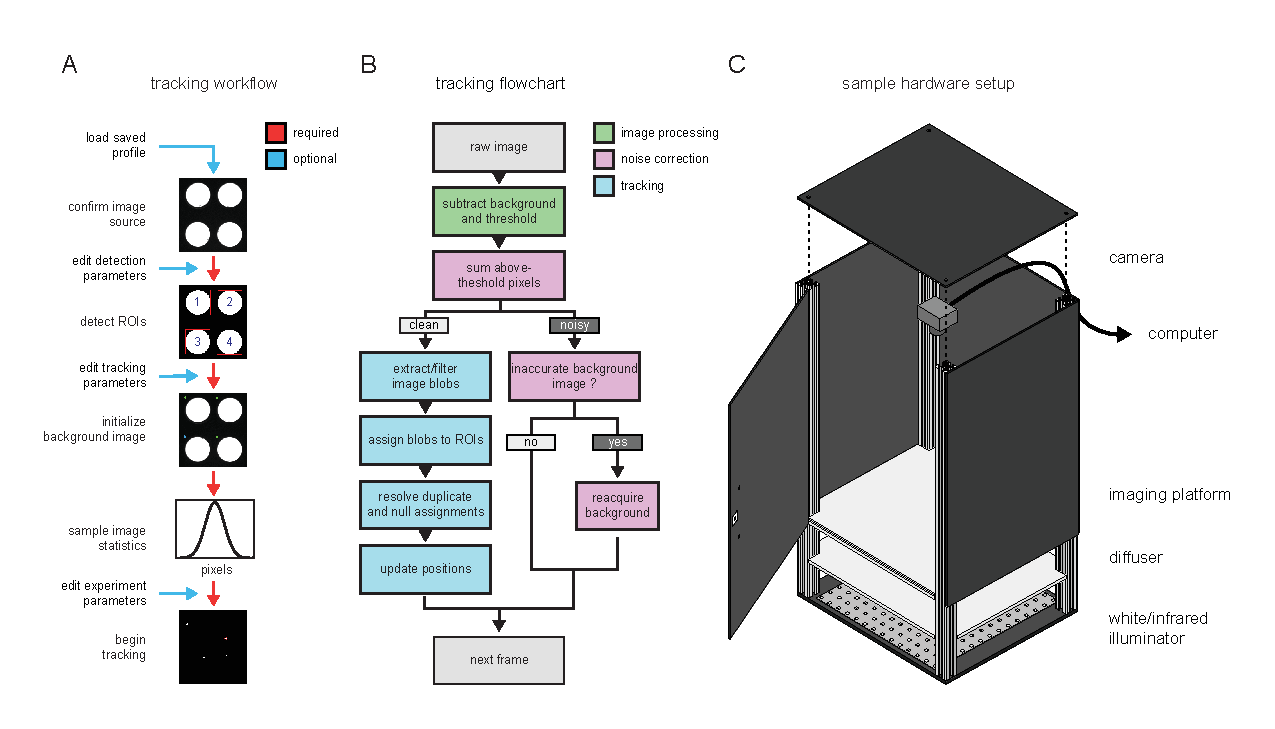
\includegraphics[width=\textwidth]{../figures/chapter_2/fig_2-1.pdf}
    \vspace{.1in}
    \caption*{\textbf{Figure 2.1} MARGO workflow, tracking algorithm, and sample behavioral box -- A) Diagram of the user workflow to set up a new tracking experiment. Arrow color indicates whether the setup step is required. Before tracking, users define an input source, define ROIs to track, initialize a background image used to separate foreground and background, and sample the image statistics on a reference of clean tracking. Tracking parameters can be customized at multiple points (blue arrows). B) Flowchart depicting the MARGO's frame-to-frame tracking routine. Each frame consists of image processing (green) to segment foreground from the background, noise estimation (magenta) to assess the quality of foreground segmentation and determine if the current frame can be tracked, and tracking (cyan) of foreground binary blobs. MARGO's tracking algorithm skips noisy frames and re-acquires the background image if many consecutive frames are deemed too noisy to track. C) Schematic of a typical behavioral box used for tracking. Behavioral arenas are backlit with an LED illuminator and imaged with an overhead camera. The tracking camera is fitted with an infrared filter to allow light visible to the animals to be controlled independently of the tracking illumination. A diffuser panel between the LED backlight and the behavioral arenas makes the illumination even. The camera and illuminator are both connected to a computer for real-time tracking and control via MARGO.}
\end{figure}

Following ROI definition, a background image is constructed for each ROI separately. Each background image is computed as the mean or median (as configured by the user) image from a rolling stack of background sample images. Tracking is performed by segmenting binary blobs from a thresholded difference image computed by subtracting each frame from an estimate of the background (figure 2.1b). Background subtraction commonly suffers from two issues with opposing solutions. The first is that subtle changes in the background over time introduce error in the difference image, requiring continuous averaging or reacquisition of the background image. The second is that continuous averaging or reacquisition of the background can make inactive animals appear as part of the background rather than foreground, making them undetectable in the thresholded difference image. Constructing the reference for each ROI separately mitigates these concerns by allowing the reference to be constructed in a piece-meal fashion by adding a background sample image only when the animals have moved from the positions they occupied in previous images of the background stack. The time needed to establish a background image depends on the activity level of the animals and the number of images in the reference stack. We typically find that 3-30 seconds are needed to initialize the background image. Once a background image is established, tracking can begin. In each frame, candidate blobs are identified as the blobs that are both 1) between minimum and maximum size threshold and 2) located within the bounds of an ROI. Candidate blobs are subsequently assigned to ROIs by spatial location. Within each ROI, candidate blobs are matched to centroid traces by minimizing the total frame-to-frame changes in position within each ROI.If the number of candidates exceeds the number of traces in a given ROI, only the candidates closest to the last centroid positions of the traces are assigned. If the number of traces exceeds the number of candidates, the candidates are assigned to the closest traces and any remaining traces are assigned no position (i.e. NaN) for that frame.

Degradation of difference image quality over time (due changes in the background, noisy imaging, and physical perturbation of the imaging setup) constitutes a significant barrier to long term tracking \cite{Sridhar_2019}. To address this problem, MARGO continuously monitors the quality of the difference image and updates or reacquires the background image when imaging becomes noisy. We refer to this collective process as noise correction. Prior to tracking, MARGO samples the distribution of the total number of above-threshold pixels under clean imaging conditions to serve as a baseline for comparison. During tracking, the software then continuously calculates that distribution on a rolling basis and reacquires a background image when the rolling sample substantially deviates from the baseline distribution.

\subsection*{\textit{Tracking accuracy and noise robustness}}

We performed a number of experiments and analyses to assess MARGO's robustness to tracking errors and comparability with other trackers. In these experiments, we tracked individual flies, each alone in a circular arena, so that individual identity was assured by spatial segregation.

We assessed the ability of MARGO to handle degradation of the difference image by repeatedly shifting the background image by a small amount in a random direction (2px, 2\% of the arena diameter, and 0.16\% of the width of the image) to mimic situations where an accidental nudge or vibration shifts the arena. MARGO was used to simultaneously record a movie of individual flies walking in circular arenas and track their centroids. These tracks were the ground truth for this misalignment experiment, and background shifting was implemented digitally on the recorded movie. MARGO reliably detects the changes in difference image statistics associated with each of these events and recovers clean tracking by reacquiring the background, typically within 1 second (figure 2.2). Forcing reacquisition of the background image has the disadvantage of resetting the reference with a single image, meaning that a normal background image built by median-filtering multiple frames spaced in time cannot be computed immediately (background images made this way have two benefits: lower pixel noise and fewer tracking dead spots because they do not include moving animals). This typically caused a reduction in tracking accuracy that is brief ($<$2s) and had little effect on the overall correlation of the tracking data to the ground truth (r=0.9998). Indeed, we found a small effect on tracking error (mean 3.07+/- 2.5 pixels, which corresponds to ~20\% of a fly's body length at our typical imaging resolution) even when shifting the background every 2 seconds. In our experimental set-ups, noise-induced background reacquisition was relatively rare, typically occurring fewer than 10 times over the duration of a two hour experiment.

\begin{figure}[t!]
 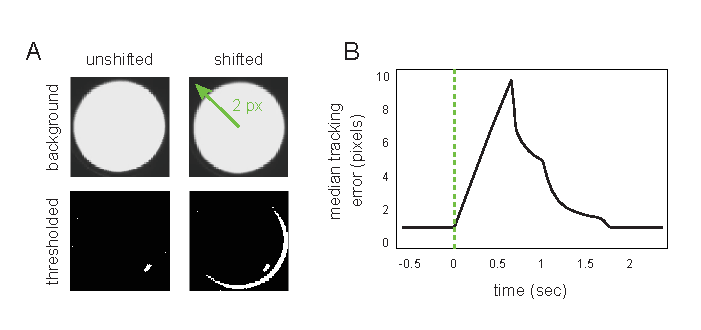
\includegraphics[width=\textwidth]{../figures/chapter_2/fig_2-2.pdf}
 \vspace{.1in}
 \caption*{\textbf{Figure 2.2} -- A) Diagram of the background image shifting scheme used to simulate the kind of background inaccuracy that can happen in long experiments. B) Trial-triggered median tracking error centered on reference shifting.}
\end{figure}

We tested MARGO's sensitivity to video compression by compressing and tracking a video previously captured during a real-time tracking session. The centroid position error of traces acquired from compressed videos were calculated by comparing them to the ground-truth traces acquired on uncompressed images in real time. MARGO showed sub-pixel median tracking error up to 3000-fold compression (figure 2.3a). We further tested the robustness of MARGO to noisy imaging by digitally injecting pixel noise (by randomly setting each pixel to True with a fixed probability) into the thresholded difference image of each frame of a video previously acquired and tracked under clean conditions. Noise was added downstream of noise correction and upstream of tracking to simulate tracking under conditions where noise correction is poorly calibrated. We observed sub-pixel median tracking error up to 20\%pixel noise (figure 2.3b). In practice, we find it easy to create imaging conditions with noise levels <1\% pixel noise without the use of expensive hardware.

\begin{figure}[t!]
 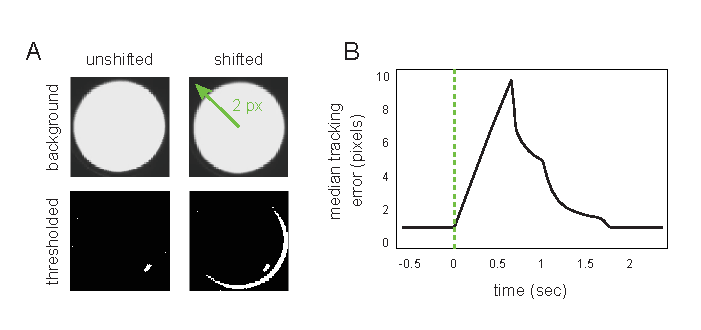
\includegraphics[width=\textwidth]{../figures/chapter_2/fig_2-3.pdf}
 \vspace{.1in}
 \caption*{\textbf{Figure 2.3} -- A) Median error of tracking performed on the same video at different levels of compression. Below: sample images. B) Median tracking error versus different levels of added noise. Pixel noise was manually added to the binary threshold image downstream. Below: sample images with estimated fly position (red circle).}
\end{figure}

To compare the tracking accuracy of MARGO to a widely used animal tracker, we fed uncompressed video captured during a live tracking session in MARGO into Ctrax \cite{Branson_High_2009} and measured the discrepancy between the two sets of tracks. Overall we found a high degree of agreement between traces acquired in MARGO and Ctrax (figure 2.4). We attribute the majority of discrepancies to minor variations in blob size and shape arising from differences in background segmentation. It is worth noting that although Ctrax flagged many frames for manual inspection and resolution, for comparability we opted not to resolve these frames and instead restricted our analysis to the automatically acquired traces. (Ctrax primarily uses these flags to draw user attention to tracking ambiguities through collisions, which did not happen in our experiment because flies were spatially segregated.) Manual inspection of tracked frames with error larger than 1 pixel revealed that most major discrepancies occurred in one of two ways: 1) short periods between the death and birth of two traces on the same animal in Ctrax, or 2) identity swaps in Ctrax between animals in neighboring arenas. These errors may be attributable to our inartful use of Ctrax.

\begin{figure}[t!]
 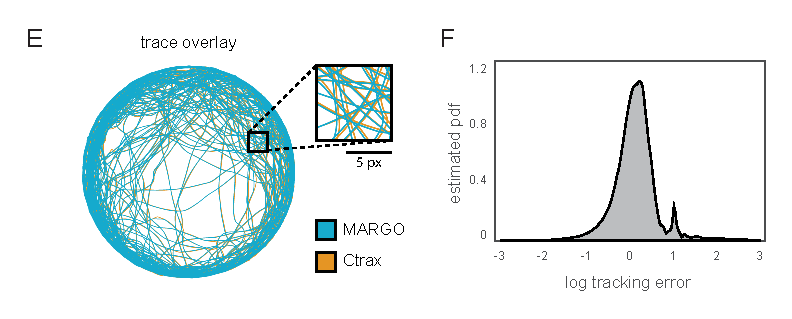
\includegraphics[width=\textwidth]{../figures/chapter_2/fig_2-4.pdf}
 \caption*{\textbf{Figure 2.4} -- A) Sample trace comparison and B) log distribution of tracking error between traces acquired from the same video in both MARGO and Ctrax.}
\end{figure}

\subsection*{\textit{High-throughput behavioral screens}}

We designed MARGO with high-throughput behavioral screens in mind, with hundreds of experimental groups, each potentially containing hundreds or thousands of animals. Many features in MARGO's GUI have been included to reduce the time needed to establish successful tracking, including automated ROI detection and visualizations of object statistics and the effects of parameters. Configuring tracking for experiments with hundreds of individuals typically took between 2-5 minutes. Additionally, we added the ability to save and load parameter and experimental configurations.

\begin{figure}[b!]
 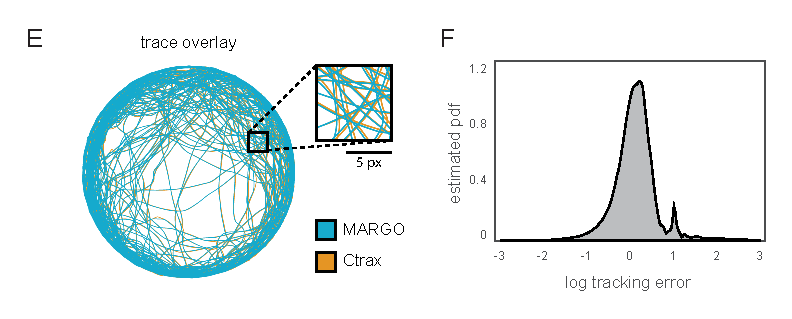
\includegraphics[width=\textwidth]{../figures/chapter_2/fig_2-5.pdf}
 \vspace{.1in}
 \caption*{\textbf{Figure 2.5} -- A) Image of 10 single-fly housing plates from the overhead tracking camera. B) Sample tracks from the same fly on days 1 and 6.}
\end{figure}

The speed of the tracking algorithm permits the tracking of very large numbers of animals simultaneously in a single field of view (facilitating certain experimental designs, like testing multiple experimental groups simultaneously). To demonstrate MARGO's throughput, we continuously tracked 960 flies at 8Hz for more than 6 days (supplemental video 1). Flies were singly housed in bottomless 96-well plates (figure 2.5a) placed on top of food and were imaged by a single overhead camera. The appearance of the arenas changed substantially over 6 days due to evaporation of water from the fly food media, condensation on the well plate lids, and egg laying. Despite these changes, the quality of centroid traces and acquisition rates appeared stable throughout the experiment (figure 2.5b). The overall activity level of flies decreased over the duration of the experiment (figure 2.6). The flies' log-speed distributions generally exhibited two distinct modes: a low mode consistent with frame-to-frame tracking noise and a higher mode consistent with movement of the flies (figure 2.7a) \cite{berman_choi_bialek_shaevitz_2014,Crall_2016_cockroach}. Individual flies varied in the relative abundance of these two modes. We defined a movement threshold as the local minimum between these two modes and parsed individual speed trajectories into movement bouts by identifying periods of continuous movement above the threshold. Sorting flies by the average length of their movement bouts revealed a trend of increasing mean and magnitude of the higher "movement" mode (figure 2.7a), i.e., flies that walked longer tended to walk faster.

\begin{figure}[t!]
 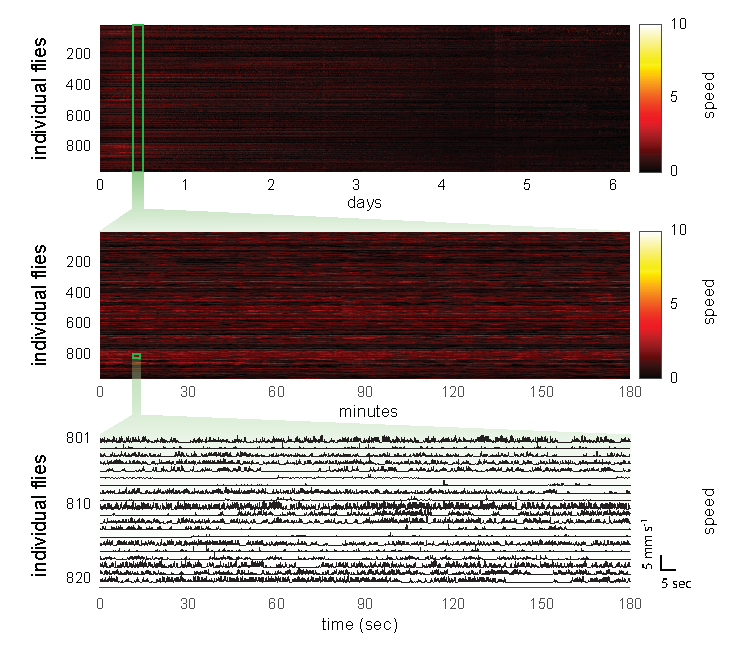
\includegraphics[width=\textwidth]{../figures/chapter_2/fig_2-6.pdf}
 \caption*{\textbf{Figure 2.6} -- Fly speeds at three representative scales: heatmap of individual speed over the duration of the experiment (top), heatmap of individual speed from a three hour period (middle), raw speed traces from twenty individuals from a three minute period (bottom). Activity of most flies decreased over the six day duration.}
\end{figure}

To measure MARGO's performance as a function of the number of ROIs, we recorded the mean real-time tracking rate while varying the number of tracked ROIs from a high-resolution (7.4MP) video composed of the same single-arena video repeated 2400 times in a grid. We found that the frame-to-frame latency scaled linearly as a function of the number of ROIs tracked (figure 2.7b). On modern computer hardware (intel i7 4.0GHz CPU), we measured tracking rates of 160Hz for a single ROI down to 5Hz for 2400 ROIs. MARGO could plausibly track up to 5000 animals at lower rates (~1 Hz), potentially fast enough for experiments monitoring changes in activity level changes over long timescales, like circadian experiments.

Large behavioral screens can potentially generate hundreds of hours of data on thousands of animals and massive data files even without recording videos. We found that experiments tracking many hundreds of animals over multiple days made raw data files too large to hold in memory on typical computers. We designed a custom data container and an API to easily work with data stored in large binary files. MARGO's raw data API includes methods to batch-process multiple tracking experiments or single datasets too large to hold in memory (see user documentation).

\begin{figure}[t!]
 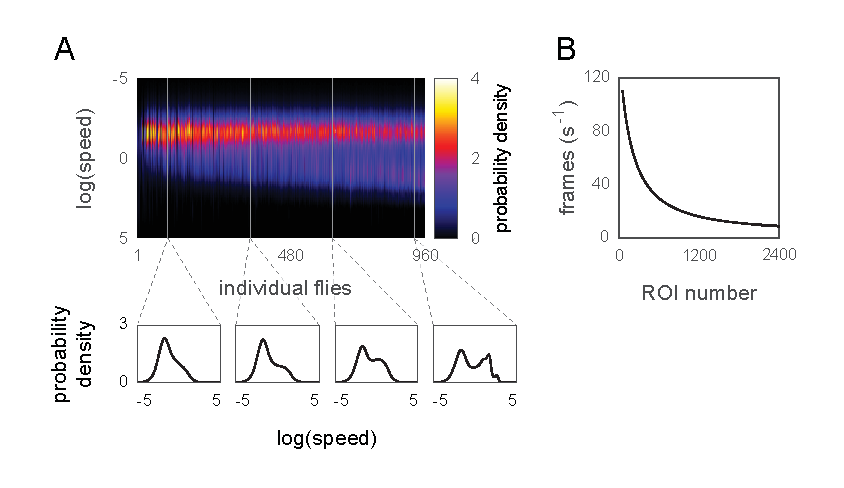
\includegraphics[width=\textwidth]{../figures/chapter_2/fig_2-7.pdf}
 \vspace{.1in}
 \caption*{\textbf{Figure 2.7} -- A) Individual kernel density estimates of log speed over the duration of the experiment. Column order was sorted by mean individual bout length in ascending order. B) Acquisition frame rate as a function of number of ROIs tracked in a simulated experiment. The acquisition rate decreased exponentially, consistent with a linear increase in inter-frame interval as a function of ROI number.}
\end{figure}

\subsection*{\textit{Customization and versatility}}

To demonstrate MARGO's ability to prototype experiments without the need for specialized hardware, we ran a minimal tracking experiment using only commonly available materials. Individual fruit flies were placed into the wells of a standard 48 well culture plate. The plate was put in a cardboard box (to reduce reflections) on a sheet of white paper as a high contrast background. Movies were recorded on a 1.3MP smartphone camera using natural room light as illumination and imported into MARGO for tracking (supplemental video 2). Tracks and movement bouts acquired under these conditions showed no apparent differences to those acquired under our normal experimental conditions (custom arenas over diffused LED illuminators in light-sealed imaging boxes). However, we did find that the lower contrast illumination of this setup increased imaging noise and narrowed the range of parameters that worked for segmentation, but had no apparent effect on the accuracy of traces once calibrated.

MARGO was developed for high-throughput ethology in fruit flies, but many small organisms used for high-throughput behavior are more translucent than adult flies. To assess MARGO’s tracking robustness on such organisms, we used MARGO to track videos of larval \emph{Danio rerio}, \emph{Caenorhabditis elegans}, larval \emph{Drosophila} (supplemental videos 3-5), and also bumblebees (\emph{Bombus impatiens}) (supplemental videos 6). As expected, the translucency of these organisms narrowed the functional range of some tracking parameters, but MARGO's real-time tracking feedback made it easy to dial in these parameters. Sample traces acquired from other organisms were qualitatively similar to those acquired with adult flies, suggesting that MARGO works with a variety of organisms.

We gave MARGO a graphical user interface (GUI) to make it accessible to users unfamiliar with MATLAB or programming in general (figure 2.8). We generally find that new users easily learn to use both the core work-flow and parameter customization. The typical setup time of a tracking experiment for trained users ranged between a few seconds (with saved parameter profiles) to a few minutes (under novel imaging conditions). The utility of the GUI extends to customization of analysis, visualization, and input/output sources such as videos, cameras, displays, and COM devices. Descriptions and instructions for these use cases, including defining custom experiments via the API, are available in MARGO's documentation.

D) Representative views of MARGO's GUI. Blue inset shows the controls for setting tracking parameters, pink inset the menu options for configuring experiments.

\begin{figure}[t!]
    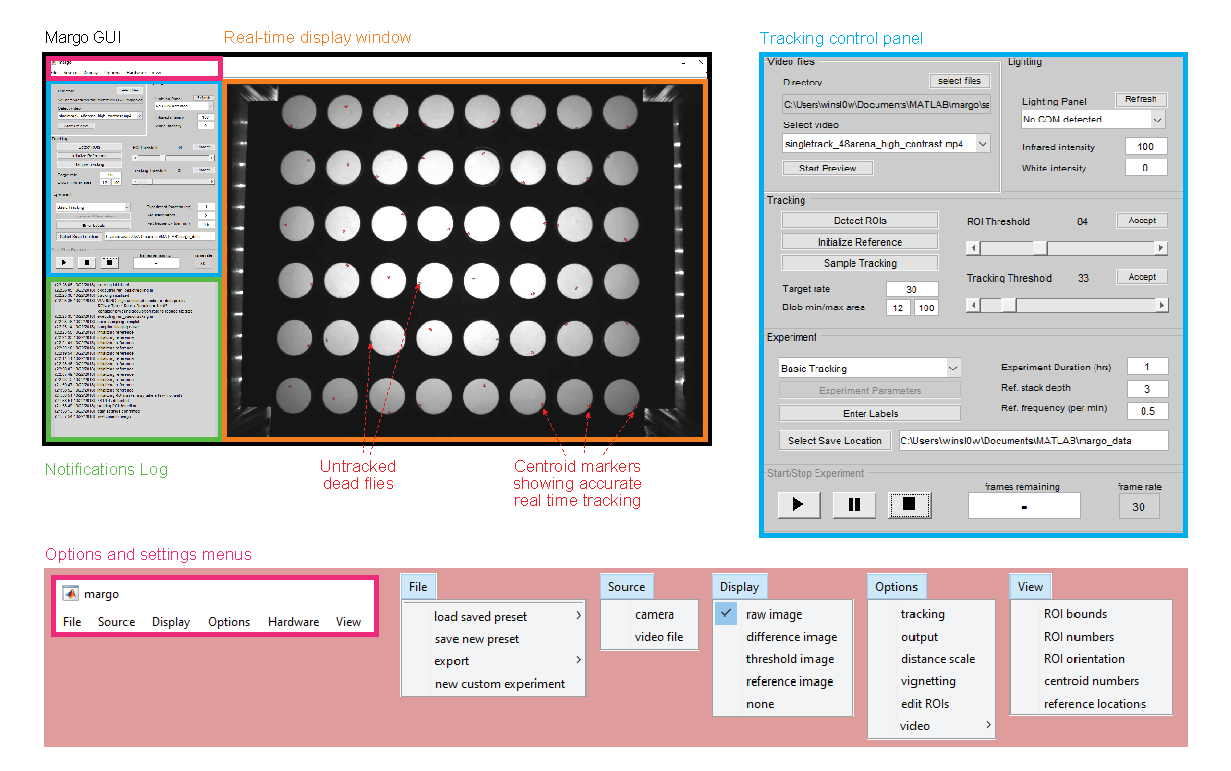
\includegraphics[width=\textwidth]{../figures/chapter_2/fig_2-8.pdf}
    \vspace{.1in}
    \caption*{\textbf{Figure 2.8} Representative views of MARGO's GUI. Blue inset shows the controls for setting tracking parameters, pink inset the menu options for configuring experiments.}
\end{figure}

\subsection*{\textit{Integrating hardware for closed-loop experiments}}

Real-time tracking allows the delivery of closed-loop stimuli that depend on the behavior of animals. MARGO offers native support for the hardware needed for closed-loop experiments including: cameras for real-time image acquisition, projectors/displays for visual stimuli, and serial COM devices for digital control of other peripheral electronics. COM devices include programmable microcontrollers (like Arduinos) that make it relatively simple to control a wide variety of devices. MARGO was designed to detect and communicate with such COM devices devices to integrate real-time feedback from sensors and coordinate closed-loop control of peripheral hardware. 

We ran experiments with a custom circuit board to measure individual phototactic preference (the "LED Y-maze"). In this assay, individual flies explored symmetrical Y-shaped arenas with LEDs at the end of each arm (figure 2.9a-b, supplemental video 7). For all arenas in parallel, real-time tracking detected which arm the fly was in at each frame. At the start of each trial, an LED was randomly turned on in one of the unoccupied arms. Once the fly walked into one of these two new arms, MARGO turned off all the LEDs in that arena. Immediately after these choice events, a new trial was initiated by randomly turning on an LED in one of the now unoccupied arms. This process repeated for each fly independently over two hours, and MARGO recorded which turns were toward a lit LED (positive phototaxis) and which were away (negative phototaxis) (figure 2.9c). Tiling many such mazes on a single board yielded the experimental throughput for which MARGO is well-suited. Overall, we recorded choices from over 3,600 individuals, representing more than 830,000 choices in total.

\begin{figure}[t!]
 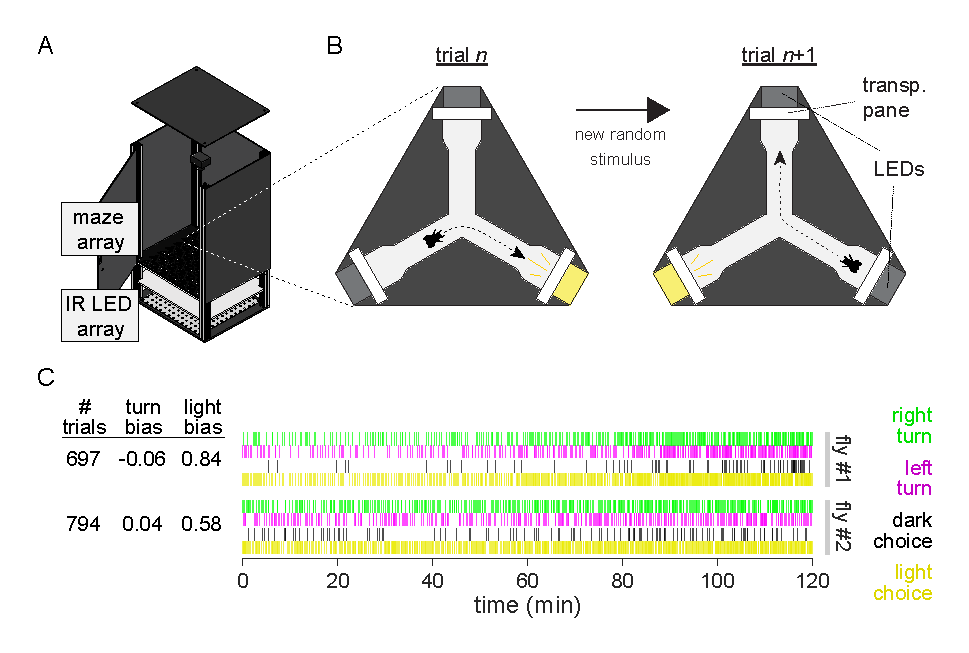
\includegraphics[width=\textwidth]{../figures/chapter_2/fig_2-9.pdf}
 \vspace{.1in}
 \caption*{\textbf{Figure 2.9} -- A) Schematic of the behavior box with an LED Y-maze array in place. B) Diagram of a single LED Y-maze and trial structure. New trials initiate by turning on (yellow) an LED in one of the two unoccupied maze arms. The trial ends when then animal turns into a new arm and the lit LED is turned off (gray). Each turn is scored for both handedness and phototactic preference. C) Raw turn data for two sample flies. Each individual trial consists of both a phototactic and handedness choice. Individual mean turn biases range from 0 (all left turns) to 1 (all right turns). Light biases range from 0 (all photopositive turns) to 1 (all photonegative turns).}
\end{figure}

To assess MARGO's capacity to reveal behavioral differences between genotypes, we tested a variety of wild type strains in the LED Y-maze. All strains exhibited a significant average positive phototactic bias (mean phototactic indices ranging from 0.55 to 0.80, p-values$<<$10$^{-6}$ by t-test). In contrast, blind flies (\emph{Norp-A} mutants) and flies under identical circumstances but with unpowered LEDs, showed mean "preferences" indistinguishable from 0.5, consistent with random choices (figure 2.10a). The wild type lines tested showed significant variation in population mean (one-way ANOVA; F(6,1943)=118.2, p$<<$10$^{-6}$) and population variability (one-way ANOVA on Levene-transformed data; F(6,1943)=19.29, p$<<$10$^{-6}$).

We collected LED Y-maze data from a single cohort of wild-type (Berlin-K, n=144) flies over the first 8 days post-eclosion to profile phototaxis throughout development (figure 2.10b). Flies displayed a significant average negative light bias (0.417, p$<<$10$^{-6}$) on the day of eclosion but transitioned to a positive light bias of 0.663 (p$<<$10$^{-6}$) by 7 days post-eclosion. This assay has structural similarities to an assay we previously used to measure locomotor handedness \cite{Buchanan_Neuronal_2015}, the tendency of individuals to turn left or right when going through the center of the arena. In the LED Y-maze assay, locomotor left-right decisions were made in superposition with light-dark choices. Flies typically make hundreds of choices over the course of an experiment, giving us enough data to examine the turn bias of individuals in all four left-right/light-dark combinations. We divided trials into two groups based on whether the lit LED appeared to the right or left of the choice point. We found that the mean turn bias but not the mean phototactic bias differed between these two conditions (figure 2.10c) \cite{Ayroles_Behavioral_2015}. Categorizing trials this way revealed that the rank order of both turn bias and phototactic bias are anti-correlated (r=-0.38 and r=-0.63 respectively) between the two conditions, suggesting that both individual phototactic bias and locomotor handedness bias affect each choice.

\begin{figure}[t!]
 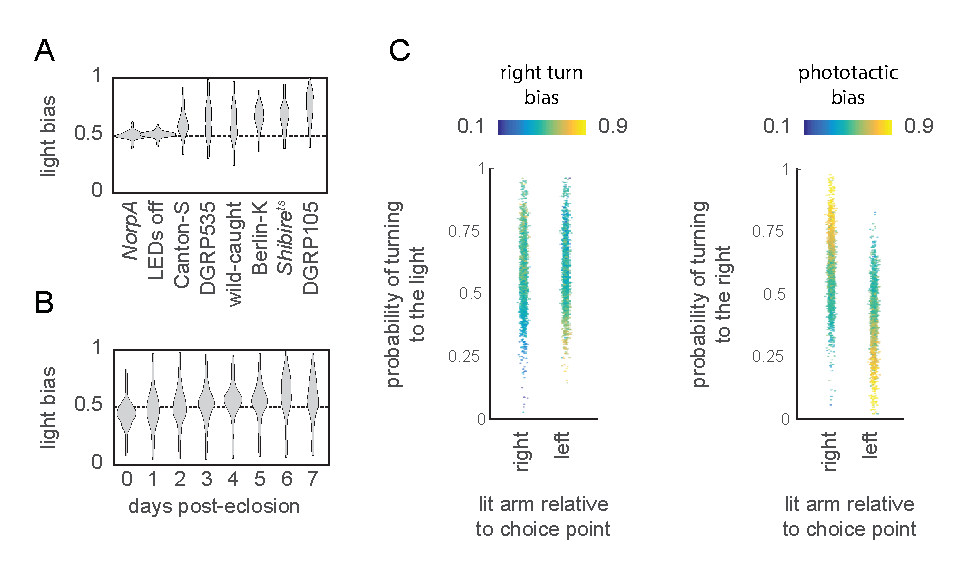
\includegraphics[width=\textwidth]{../figures/chapter_2/fig_2-10.pdf}
 \vspace{.1in}
 \caption*{\textbf{Figure 2.10} -- A) Comparison of individual average phototactic bias distributions for different wild-type fly lines. Blind flies (NorpA) and flies tested with all LEDs turned off (DGRP-105 dark) are included as negative controls. Horizontal dashed line indicates random bias at p=0.5. B) Distribution of individual average phototactic biases for the same cohort of flies over the first 8 days post-eclosion. C) Individual mean phototactic and right turn biases calculated on all trials sub-divided by into trials where the lit arm of the maze was to the right or left of the choice point. Data points are colored by either the individual mean right turn bias (left panel) over all trials or the individual mean phototactic bias (right panel) over all trials. The rank orders of both turn bias and phototactic bias are anti-correlated (r=-0.38 and -0.63 respectively) between trials where right or left arm was lit}
\end{figure}

We adapted an optomotor paradigm \cite{Cruz572792} to a high-throughput configuration to test MARGO's ability to deliver a precise closed-loop stimulus with low latency. In this paradigm, an optomotor stimulus consisting of a high-contrast, rotating pinwheel, centered on a fly, is projected on the floor of the arena in which it is walking freely. On average, such optomotor stimuli evoke a turn in the direction of the rotation to stabilize the visual motion \cite{Gtz_Visual_1973}. The center of the pinwheel follows the position of the fly as it moves around the arena so that the only apparent motion of the stimulus is around the fly. Thus, this stimulus is closed-loop with respect to each animal's position and open-loop with respect to its rotation velocity.

To implement this paradigm, we constructed a behavioral platform with a camera and an overhead mounted projector targeting an array of flat circular arenas (figure 2.11a-b). To target a stimulus to a fly based on its coordinates in the tracking camera, MARGO had to learn the mapping of camera coordinates to projector coordinates. We added a feature to locate small dots displayed by the projector with the camera. From the position of these dots in camera coordinates, we constructed a registration mapping from the camera FOV to the projector display field. Using this mapping, we programmed MARGO to use the real-time positions of flies to project pinwheel stimuli independently to 48 freely moving individuals simultaneously (fig. 5B, supplemental video 8). To ensure faithful coordination between the tracking and stimulus, the tracking rate was matched to the refresh rate of the display at 60Hz (which is below the flies' flicker-fusion rate, meaning this stimulus produces beta movement apparent motion \cite{haag_arenz_serbe_gabbiani_borst_2016}; see Discussion). 

\begin{figure}[t!]
 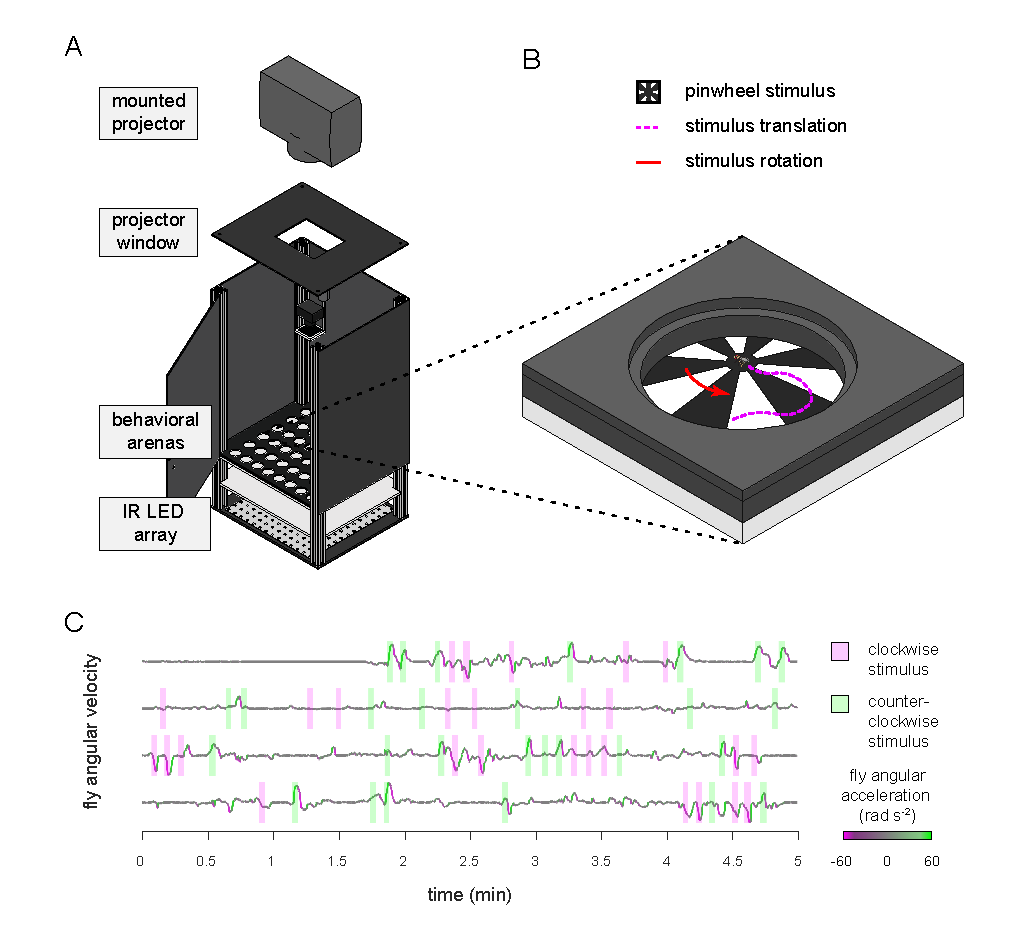
\includegraphics[width=\textwidth]{../figures/chapter_2/fig_2-11.pdf}
 \caption*{\textbf{Figure 2.11} -- A) Schematic of the optomotor arenas and behavioral box. B) Diagram of a single arena and optomotor stimulus. Trials begin with a pinwheel stimulus, centered on the fly. For each trial, the rotational direction (red arrow) of the stimulus is randomized. As the animal moves, the pinwheel position is updated to stay centered on the fly. Trials end when the stimulus is removed after 2 s. C) Four sample raw individual angular velocity time series. Flies typically respond to optomotor stimuli by turning in the direction of the rotation of the stimulus. Shaded rectangles indicate the direction of pinwheel rotation, line color angular acceleration. Hundreds of individual trials are recorded on average over a two hour period.}
\end{figure}

While optimizing this assay, we observed that optomotor responses could be reliably elicited, provided individuals were already moving when the pinwheel was initiated. This is consistent with previous observations of optomotor responses depending on arousal state \cite{Zhu_Peripheral_2009,Kim_Fly_2016}. We therefore configured MARGO to stimulate with the pinwheel each fly when: 1) it was moving 2), a minimum inter-trial interval had passed, and 3) it was a minimum distance away from the edge of the arena. The inter-trial interval helped prevent behavioral responses from adapting, and provided a baseline measurement period where no stimulus was present. Minimum distance to the edge ensured that the stimulus occupied a significant portion of the animal's field of view. 

We characterized the optomotor behavior of wild type flies in a two hour experiment with two second pinwheel stimuli and a minimum inter-trial interval of 2s (figure 2.11c). In total, over 300,000 trials were recorded from more than 1,800 flies, assayed in groups of up to 48 flies simultaneously. For each fly, we calculated an optomotor index \cite{Seelig_Two_2010} as the fraction (normalized to [-1,1]) of body angle change that occurred in the same direction as the stimulus rotation over the duration of the stimulus. On average, flies displayed reliable optomotor responses (mean index = 0.358, p$<<$10$^{-6}$) when stimulated with high-contrast pinwheels (figure 2.12a). We observed significant individual variation in optomotor index (figure 2.12b) as well as the number of trials each fly experienced, reflecting individual variation in the fraction of time walking. 

\begin{figure}[t!]
 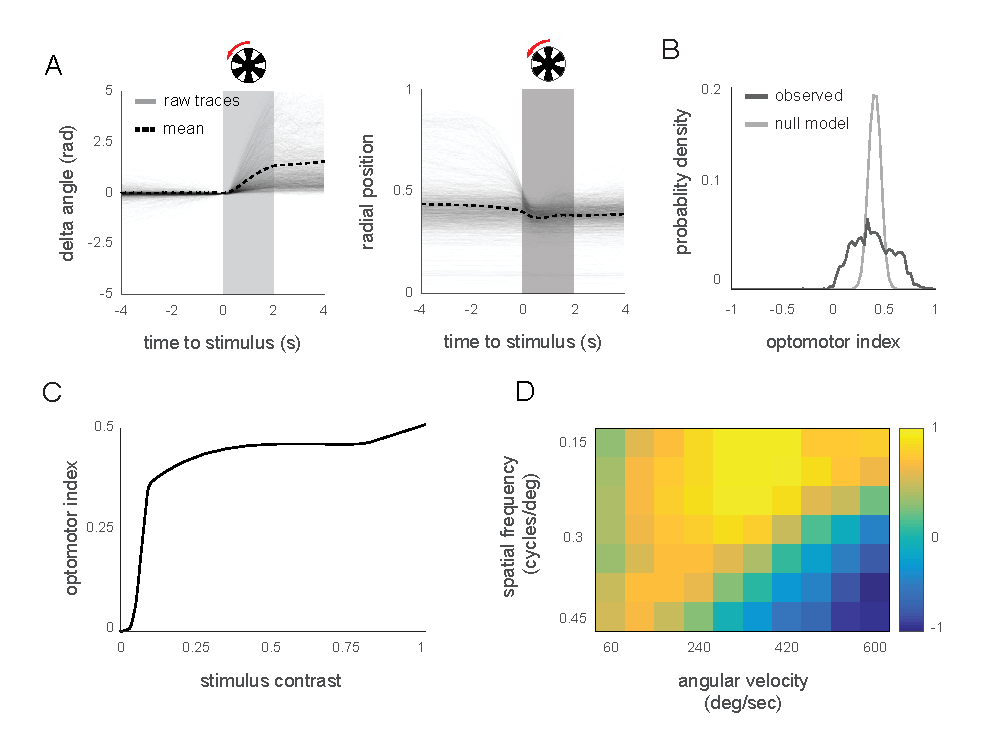
\includegraphics[width=\textwidth]{../figures/chapter_2/fig_2-12.pdf}
 \caption*{\textbf{Figure 2.12} --  A) Trial-triggered average optomotor response across all individuals. Change in body angle (left) is scored as positive or negative relative to the rotational direction of the stimulus. All trials were aligned to have change in body angle of zero at the onset of the stimulus. Average distance to the arena center (right) drops immediately preceding stimulus onset due to the requirement that flies must be off the arena edge to start a trial. B) Comparison of the observed distribution of individual average optomotor indices (n=1,860) to the distribution expected under a null model in which all flies turn with identical statistics, generated by bootstrap resampling. C) Population average optomotor index as a function of stimulus contrast (0-1). Pinwheel contrast was randomly varied on a trial-by-trial basis. D) Average optomotor index as a function of stimulus spatial frequency and stimulus angular velocity.}
\end{figure}

To characterize the psychometric properties of this behavior, we randomly varied pinwheel contrast, angular velocity, and spatial frequency simultaneously on a trial-by-trial basis. Mean optomotor indices increased with pinwheel contrast, plateauing over much of the dynamic range of the projector, starting around 25\% contrast (figure 2.12c). Similarly, optomotor indices increased with both stimulus spatial frequency and angular speed, peaking at 0.18 cycles/degree and 360 degrees/s respectively (figure 2.12d). The population mean optomotor index reversed at high combined values of spatial frequency and angular speed due to the apparent reversal of the stimulus at frequencies higher than the refresh rate of the projector.

\subsection*{\textit{High-throughput optogenetic experiments}}

To test the versatility of MARGO, we used its API to implement high-throughput closed-loop optogenetic experiments using a digital projector to target individual flies expressing CsChrimson \cite{griebel_2014,Klapoetke_Independent_2014} with flashing red light contingent on their behavior (fig. 6). We used a commericial Optoma S310e DLP projector which, when displaying red light ([255 0 0] RGB code), had a spectral range of 570 nm to 720 nm with a peak at 595 nm. Light stimulation frequency was set to the projector refresh rate (60Hz) and its intensity to the maximum, if not otherwise specified.

\begin{figure}[t!]
 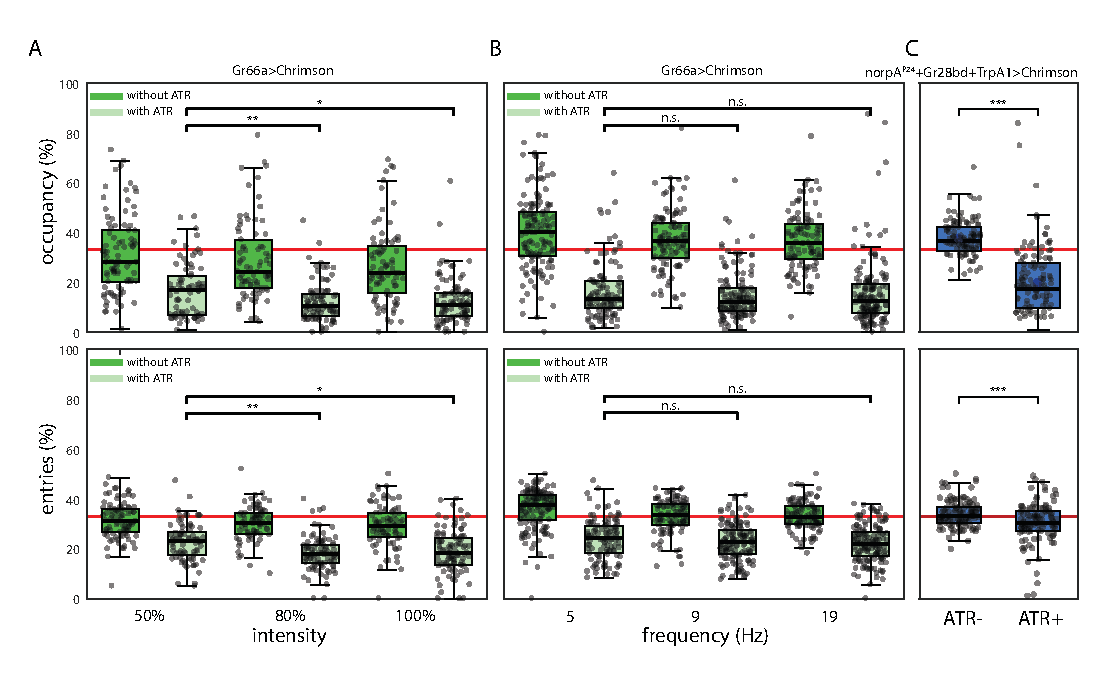
\includegraphics[width=\textwidth]{../figures/chapter_2/fig_2-13.pdf}
 \caption*{\textbf{Figure 2.13} --  A) Top: Fraction of time spent in the arm of a Y-maze which was triggered to optogenetically stimulate flies expressing CsChrimson in bitter taste receptor neurons. Bottom: Portion of arm entries into the reinforced arm. Light green boxes are control flies not fed ATR; dark green experimental flies are fed ATR. Red line indicates chance rates. Individual points are flies. Even at the lowest intensity (50\%), flies show a robust avoidance of the reinforced arm in a Y-Maze. Increasing light intensity (x-axis) further decreases (slightly) the lit arm occupancy time and the lit arm entries even further. Here and elsewhere *:p<0.05, **:p<0.01, ***:p<0.001. *:p<0.05, **:p<0.01, ***:p<0.001. B) As in A.1, but varying the frequency of the optogenetic stimulation. Frequency had little effect on the occupancy or rate of entry into the reinforced arm. C) Blind \textit{norpA\textsuperscript{P24};Gr28bd+TrpA1>Chrimson} flies, expressing Chrimson in heat-sensitive neurons, also show decreased occupancy in the lit arm, whereas the fraction of entries into the lit arm appears unchanged compared to control flies not fed ATR. 
}
\end{figure}

As a first experiment, we tracked the flies in a Y-Maze shaped like that in fig. 4A, but with no LEDs. Whenever a fly entered a designated arm, MARGO projected red light on it. Flies expressed CsChrimson in bitter-taste receptor neurons using the driver \textit{Gr66a-GAL4}. MARGO recorded the fractional time spent in the lit arm (occupancy) and the number of entries into the lit arm (entries). We observed a modest increase in the aversive effects of optogenetic stimulation (reduced occupancy and entries) with light intensity (figure 2.13a), whereas increasing stimulation frequency did not elicit any obvious change in aversion (figure 2.13b). To test the robustness of the experiment to changes in the fictive conditioning stimulus, and to exclude the effects of visual cues, we expressed CsChrimson in heat sensitive neurons targeted by \textit{Gr28bd+TrpA1-GAL4} in \textit{norpA\textsuperscript{P24}} blind flies. This experiment is conceptually analogous to spatial learning in the heat-box, where flies are trained to avoid one side of a dark, heatable chamber \cite{wustmann_rein_wolf_heisenberg_1996,wustmann_heisenberg_1997,diegelmann_2006,ostrowski_kahsai_kramer_knutson_zars_2015,putz_2002,sitaraman_zars_zars_2007,sitaraman_zars_zars_2010,zars_zars_2006}. While blindness only marginally affected the time spent in the lit arm (the blind flies with Chrimson driven in heat-sensitive neurons still avoided occupying the lit arm at similar rates to seeing flies with Chrimson in bitter-sensitive neurons), the reduction in entries into the lit arm, observed in the seeing flies, was abolished (figure 2.13c). These results suggest that vision is a key sensory modality informing the decision to enter an arm, but not for the decision of how much time to spend in an arm, once entered.

Analogous to a different heat-box experiment \cite{YANG2013799}, optogenetic stimulation was made contingent on locomotor speed rather than position. In the same circular arenas as the optomotor experiments above (figure 2.14a), the red light was switched on under two distinct conditions enforced in separate experimental blocks: 1) whenever the walking speed of the flies exceeded a threshold of 6.8 mm/s and 2) whenever the walking speed fell below that same threshold. The overall 64 minute experimental protocol consisted of 8 periods of 8 minutes each. The periods alternated between a baseline period, where the light was permanently switched off, and the two reinforcement periods where the light was contingent on either fast walking or slow walking/resting, respectively (figure 2.14b-c). As in the heat-box experiments, flies increased their walking speed when punished for walking too slowly. However, punishing fast walking failed to significantly decrease walking speed. Reminiscent of the induction of 'learned helplessness' in yoked control animals in the heat-box \cite{YANG2013799}, flies trained with these conflicting schedules of punishment, significantly reduced their walking speed in the baseline periods without optogenetic stimulation, in comparison to control animals which did not express any CsChrimson (figure 2.14c).

\begin{figure}[t!]
 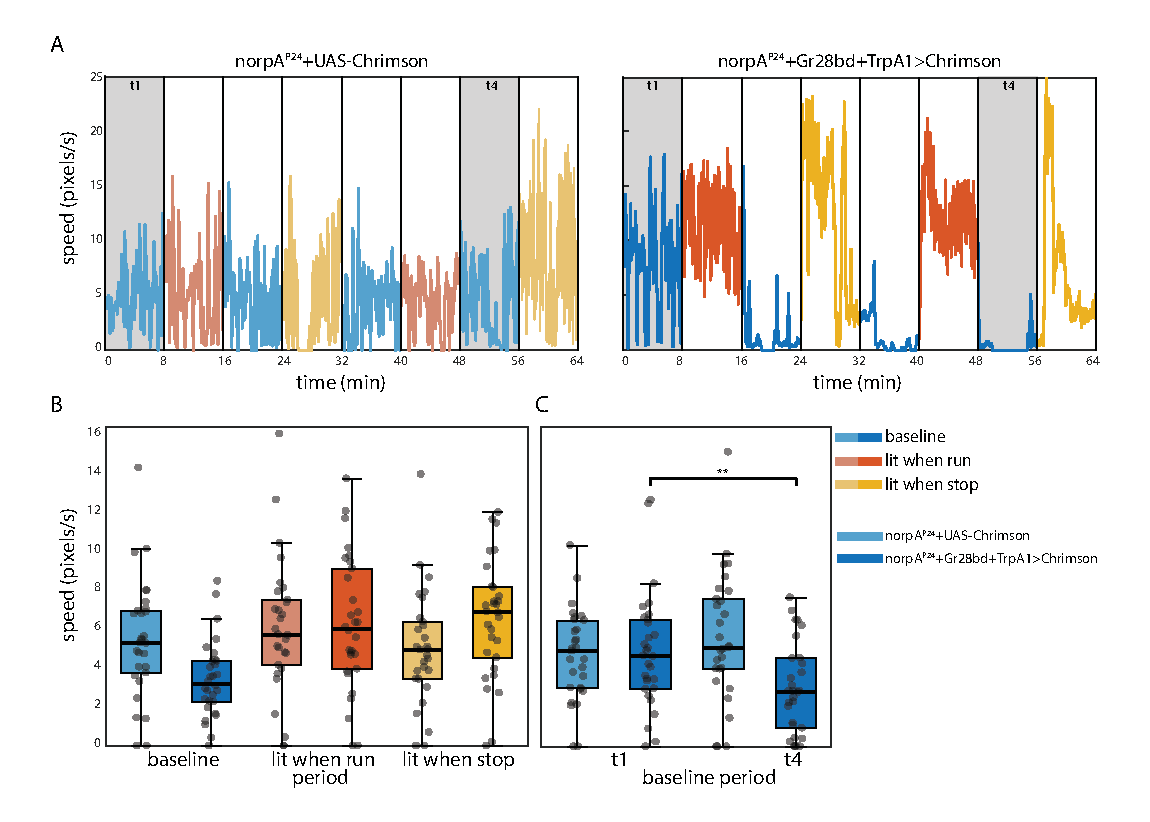
\includegraphics[width=\textwidth]{../figures/chapter_2/fig_2-14.pdf}
\caption*{\textbf{Figure 2.14} --  A) Example walking speed traces of an individual fly in circular arenas stimulated upon when above or below (depending on trial period) a speed threshold 4 px/s. Line color indicates which reinforcement paradigm was used in each period. Initial (t1) and final (t4) baseline periods are highlighted (see B.3). Green line indicates the speed threshold. B) Walking speeds for all periods and all flies. \textit{norpA\textsuperscript{P24};Gr28bd+TrpA1>Chrimson} flies increase their walking speed specifically during periods when stimulation is contingent on slow walking or resting (lit when stop), compared to lit when running periods and controls without the optogenetic effector \textit{norpA\textsuperscript{P24};UAS-Chrimson}. C) Walking speed during the initial baseline period did not differ between experimental and control flies (t1). In contrast, after three reinforcement periods, walking speed in experimental flies was significantly lower than in control flies (t4). 
All flies in B were fed with all-trans-retinal.}
\end{figure}

\section*{Discussion}
We developed MARGO as a platform for a wide variety of behavioral paradigms and organisms, all at high throughput for large-scale experiments (like genetic screens, measuring individuality and characterizing psychometric response curves). MARGO's tracking algorithm, interface, and data footprint are lightweight, making it perform well in applications like real-time centroid tracking. Conversely, it is not made for harder computational tasks like maintaining the identity of multiple animals in the same compartment. But the ability to rapidly define ROIs, and track individuals in them, enables MARGO to easily coordinate low-latency, closed-loop stimulation for psychometric and optogenetic experiments. Furthermore, by packaging MARGO in a GUI and thoroughly documenting its usage and API, we hope to make it accessible both to new users with little programming experience and advanced users developing custom experimental paradigms.

When ROI boundaries are drawn along physical barriers, individual identities can be maintained indefinitely through ROI identity, thus removing the requirement for human supervision and intervention. We found that insisting on spatial segregation ultimately relaxes the computational requirements enough that thousands of individuals can be tracked in real time. In the future, real-time tracking that maintains individual identity without physical barriers may be possible, perhaps as an extension of current methodologies that exploit neural networks to track individuals offline \cite{romero-ferrero_2019,schneider_2018}. MARGO's interface assists in the automated definition of up to thousands of ROIs. An ROI-based architecture can also be used to distinguish groups rather than individual identities by separating groups into distinct arenas. This configuration therefore allows multiple groups, as well as individuals, to be tested in parallel.

Long-term automated behavioral measurement has great potential in the fields of sleep, circadian rhythms, pharmacology, and aging, among others. MARGO offers many features useful for activity measurement over long timescales, including rapid experimental setup, small data footprint, and built-in utilities for handling large data sets. For example, over a week we tracked the behavior of 960 flies simultaneously as they walked in the wells of custom 96-well plates (figure 2.6). Such throughput can be applied to comparisons among individuals, genotypes, or treatment groups. 

With built-in hardware support for cameras, displays, and peripheral electronics, MARGO enables open- and closed-loop stimulus-evoked ethology on a large scale. Built-in features supporting projector displays, like camera-projector registration, facilitate a wide variety of visual and optogenetic experiments (figs. 5, 6). Native detection and communication with serial COM devices further extends these capabilities by providing a generic interface for a wide variety of peripheral devices, such as the LED controllers we used for the LED Y-maze (figure 2.9). Taken together, MARGO is a multi-purpose platform for coordinating hardware inputs and outputs for high-throughput ethology. 

Between our two closed-loop visual stimulation experiments (LED Y-maze and optomotor assay), we screened nearly 5,000 animals over hundreds of thousands of trials, allowing the precise characterization of both individual- and population-level behavior. With the experiments themselves representing less than a week of testing, these platforms could be used for large behavioral screens of hundreds of strains. In the LED Y-maze, we showed that individuals displayed idiosyncratic biases in both phototactic preference and locomotor handedness simultaneously, as observed previously in separate assays \cite{Kain_Phototactic_2012,Buchanan_Neuronal_2015}. The wild-type fly lines we screened displayed population level differences in both mean preference and variability in phototactic bias \cite{Ayroles_Behavioral_2015}. Furthermore, the mean of one strain (Berlin-K) shifted from negative to positive over the first week post-eclosion, as was reported previously \cite{Chiang_Tactic_1963}. Interestingly, we observed that flies with a high right-turn probability were more likely to turn toward the light when it was to the right of the choice point and that the opposite was true of flies with a high left-turn probability. We observed a similar but stronger effect of phototactic bias on locomotor handedness (e.g., flies with a high phototactic bias were more likely to turn toward the right when the light was on the right). Together these results demonstrate measurable effects of phototactic bias and handedness in a task that probes both simultaneously. Thus, we found that both individual light and handedness biases influence light/turn behavior on a choice-by-choice basis. As responses to light are ethologically relevant \cite{Kain_Variability_2015}, the interplay of individual behavioral biases may have fitness consequences for wild flies.

In the optomotor experiment, we demonstrated that, using closed-loop stimuli delivered from a projector, MARGO can quantify individual optomotor responses of dozens of flies simultaneously. Consistent with previous findings \cite{Zhu_Peripheral_2009,Kim_Fly_2016}, we saw that stationary flies did not exhibit strong optomotor responses, consistent with the idea that this reflexive behavior may be state-dependent \cite{Rosner_Behavioural_2009, Rien_Octopaminergic_2013, Chiappe_Walking_2010, Maimon_Active_2010,gorostiza_2018}. While all animals tested exhibited the optomotor response to some degree, we observed a broad distribution of individual optomotor indices, suggesting that individuals respond idiosyncratically to the same stimulus, as has been found previously in other spontaneous and stimulus-evoked behaviors \cite{Kain_Phototactic_2012,Kain_Leg_2013,Kain_Variability_2015,Buchanan_Neuronal_2015,Todd_Systematic_2017}. We suspect that the success of this assay may be partially due to tightly centering the pinwheel centered on the animal as it moves, which is possible because of MARGO's low latency.

Our optogenetic experiments provide a proof of principle that high-throughput closed-loop manipulation of neural activity is feasible. Using different driver lines to activate neurons under both spatial (figure 2.13) and locomotor (figure 2.14) contingencies, optogenetic stimulation reliably altered fly behavior in the expected directions. These experiments also revealed that flies use visual elements of the projector rig to orient when the stimulus was nominally off, and that optogenetic punishment can induce learning effects outlasting the stimulation itself. These results also remind us about a general limitation of studying freely moving animals: the large number of degrees of freedom that such behavior enables can make it difficult to causally relate biological manipulations to specific mechanisms. For instance, without prior knowledge of the function of the optogenetically targeted neurons, it would not have been immediately clear if our manipulation affected reinforcing neurons or neurons involved in motor control, which could also lead to altered occupancy of the lit arm in the Y-Maze. Likewise, a screen for neurons that are required for non-random entry into optogenetically-reinforced arms of the Y-maze would yield blind flies, as the flies in our assay apparently use visual cues to identify which arms are reinforced before entering them.

Behavioral experiments are frequently more complex than tracking objects in a dish. Such experiments could require complex arena geometries, data streams from external sensors, control of peripheral hardware, and access to measurements of behavior in real time. MARGO can manage these features, making it well-suited to implementing new behavioral paradigms. Specifically, MARGO can automatically generate templates for new experiments with custom inputs and outputs within the GUI. We have also included a tutorial for defining custom experiments in MARGO's documentation. In practice, we find that new experiments can typically be defined in one or two custom functions, given familiarity with the API.

\begin{figure}[t!]
 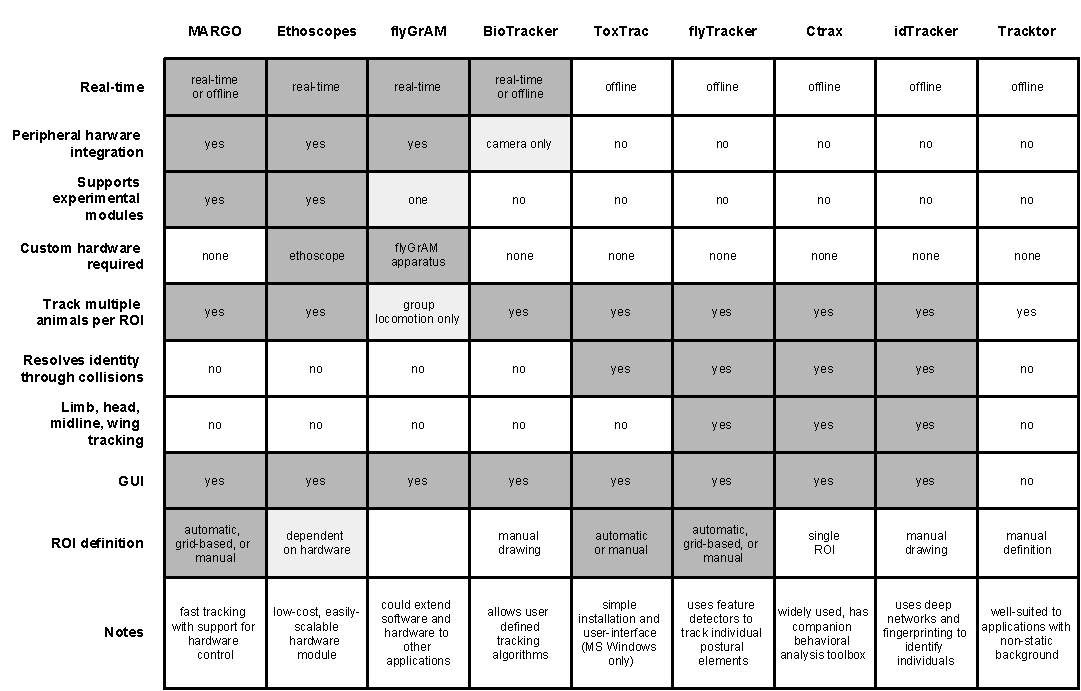
\includegraphics[width=\textwidth]{../figures/chapter_2/tab_2-1.pdf}
\caption*{\textbf{Table 2.1} -- Comparison of open-source animal tracking packages -- Trackers as falling into two rough categories: 1) real-time trackers capable of very high throughput and potential hardware integration, and 2) offline trackers capable of tracking body parts and/or maintaining individual identities without spatial segregation.}
\end{figure}

Animal tracking platforms are evolving to meet the diverse needs of the ethology, neuroscience and behavioral genetics communities. See Table 2.1 for a comparison of features of several contemporary tracking programs. Trackers can be broadly described as falling into one of two categories: 1) real-time trackers \cite{Fry_TrackFly_2008,Straw_Multi_2010,Chagas_The_2017,Geissmann_Ethoscopes_2017,Mnck_BioTracker_2018,Scaplen_Automated_2019} with potential for high throughput and hardware control and 2) offline trackers \cite{Branson_High_2009,Prez-Escudero_idTracker_2014,Eyjolfsdottir_Detecting_2014,Rodriguez_ToxId_2017,Sridhar_2019,romero-ferrero_2019} with the potential to maintain individual identities (without using spatial segregation) and/or track body parts. Hardware integration is a natural extension of real-time trackers since many stimulus paradigms are contingent on behavior. While trackers in the second category are currently unsuitable for real-time applications, they offer the notable benefits of being able to study fine-scale postural and social behaviors. The ability to record video in parallel with tracking and peripheral hardware control means MARGO can be used upstream of offline trackers, making it possible to analyze social dynamics or postural features in response to closed-loop stimuli. Among this array of options, MARGO is optimized for the throughput characteristic of \textit{Drosophila} and other genetic model organisms like \textit{C. elegans}. MARGO has the flexibility to accommodate the experimental diversity of techniques in neuroethology. Thus, we envision MARGO's niche as a versatile platform for experiments operating at high throughput to measure individual behavior and deliver closed-loop sensory and optogenetic stimuli.

% insert chapter title on its own page
\clearpage
\begin{center}
    \Large\textbf{Chapter 3}
    \thispagestyle{empty}       % set page numbering style to blank
    \clearpage
\end{center}
\section{Decathlon Screen of Individual Behavioral Variation}

\subsection{Decathlon Introduction}

Individuals display idiosyncratic differences in behavior that often persist through time and are robust to situational context. Some persistent individual behavioral traits commonly occur in correlated groups and can therefore be said to covary. Behavioral ethologists have long understood that ”types” of human and animal personalities often fall on multivariate axes of variation. . A five dimensional model \cite{goldberg_personality_1993} of known as The Big Five personality traits are frequently used by psychologists to describe the range of human personality and a similar model has been used to describe personality in fish \cite{reale_Integrating_2007}. For example, human propensity for behaviors such assertiveness, talkativeness, and impulsiveness are collectively described as extraversion and are thought to be anticorrelated with behaviors such as passivity, shyness, and deliberateness, all behaviors associated with introversion \cite{Matthews_Personality_2003}. 

In animal species, correlated suites of behaviors are described as behavioral syndromes. Aggressive behaviors such fighting over mates or food are frequently correlated with exploratory behaviors such as foraging and social interaction have been observed in insects \cite{Jeanson_Interindividual_2014}, arachnids \cite{Grinsted_Individual_2013}, fish \cite{Huntingford_Behaviour_1976}, and birds \cite{Oers_Realized_2004}. The prevalence of behavioral correlation suggests that covariation is likely a ubiquitous feature of behavior. Although correlated individual differences in behavior are commonly observed, the structure and mechanisms of behavioral covariation are not well understood. Typically, where an individual lands on these behavioral axes is thought to be determined by their individual genetic make-up. But there is increasing evidence that substantial individual behavioral variation is rooted in intragenotypic variation \cite{Honegger_Stochasticity_2018}. The extent to which intragenotypic behavioral variation is organized into syndromes or axes is essentially wholly uncharacterized. 

The particular question that motivates this study is what is the correlation structure of behavioral variation when genetic and environmental variation are minimized. Substantial variation in specific behavioral measures, even in inbred lines raised in standardized conditions has been observed in several clonal animals, including: geckoes \cite{sakai_jetho_2018}, amazonian mollies \cite{Bierbach_Behavioural_2017}, aphids and nematodes \cite{Schuett_Personality_2011,Stern_Neuromodulatory_2017}. Genetic model systems hold particular promise for the mechanistic dissection of this variation, and intragenotypic variability (IGV) in behavior has been characterized in mice \cite{Freund_Emergence_2013}, zebrafish \cite{Pantoja_Neuromodulatory_2016} and Drosophila. In flies, IGV of many behaviors has been studied, including: phototaxis \cite{Kain_Phototactic_2012}, locomotor handedness and wing-folding \cite{Buchanan_Neuronal_2015}, spontaneous microbehaviors \cite{Kain_Leg_2013,Todd_Systematic_2017}, thermal preference \cite{Kain_Variability_2015} and object-fixated locomotion \cite{Linneweber_A_2019}. Mechanistic studies of these behavioral phenomena have addressed two major questions: 1) what biological mechanisms underlie the magnitude of behavioral variability (e.g., genetic variation \cite{Ayroles_Behavioral_2015}, or neural state variation \cite{Kain_Phototactic_2012,Buchanan_Neuronal_2015}, and what specific differences within individual nervous systems predict individual behavioral biases \cite{Linneweber_A_2019}. None of these studies has focused on characterizing the large-scale variance-covariance structure of IGV in behavior. 

There is a well-developed theoretical framework for understanding the multivariate correlation structure of phenotypes. In quantitative genetics, G-matrices characterize the variance and covariance structure of phenotypes (be they behavioral, physiological, morphological) across genetically different individuals or strains \cite{Lynch_Genetics_1998}. These representations allow the quantitative prediction of responses to selection and constrain the combinations of phenotypes individuals can exhibit. Just as the phenotypic variance can be parsed into genetic variance, environmental variance,GxE interaction variance etc., covariance can be similarly dissected \cite{Charmantier_Quantitative_2014,Berdal_Adaptive_2019}. For example, phenotypic variance-covariance can be parsed as the sum of a G-matrix and an Environmental-matrix. The latter is further broken down into Temporary Environmental covariances and Permanent Environmental covariances that endure for the duration of observations. Permanent Environmental effects are those that do not arise in heritable differences, play out idiosyncratically across individuals, and are persistent. In flies, we have the potential to directly measure this component of phenotypic variance-covariance by rearing isogenic animals in standardized lab environments, profiling their individual biases over a wide range of behavioral measures, and directly measuring the variance and covariance of behavioral bias.


\subsection{Decathlon Results}

The first step in revealing the structure of behavioral variation within a genotype is to devise an experimental pipeline that produces a data set of many (200+) individual flies, with many behavioral measurements each. We first developed a number of behavioral assays, measuring both spontaneous and stimulus-evoked responses of individual flies, which could be implemented in a common experimental platform (Figure 3.1a; \cite{Werkhoven_MARGO_2019}). Using a common platform, along with choices like storing flies between experiments in 96-well plates, were important for logistical reasons, as they made maintaining the errorless identity of flies over the whole 13 day experiment substantially easier. This behavioral platform features an imaging plane, within which flies moved in arenas of various geometries. Fly position was tracked with digital cameras using diffused infrared infrared illumination invisible to the flies. Visual stimuli were presented to the animals using DLP projectors or LEDs embedded in the arena walls. We implemented six assays in this style, assessing 1) spontaneous walking in circular arenas, 2) preference to rest in higher or lower light levels (in an environment of spatially structured light), 3) preference to rest in higher or lower light levels (in a fictive, temporally-modulated light environment), 4) optomotor responses to rotating visual stripes, 5) spontaneous left-right decision making in Y-mazes, and 6) phototaxis in Y-mazes, where flies are given a choice of walking toward or away from a lit LED (Figure 3.1b). 

To these assays, we added three more, assessing 7) odor sensitivity in linear chambers \cite{Claridge-Chang_Writing_2009} in which half of the compartment is filled with an aversive odorant, 8) spontaneous behavior, acquired via high-resolution 100 Hz video and suitable for pixel-based unsupervised classification \cite{berman_choi_bialek_shaevitz_2014}, and 9) circadian activity and spontaneous locomotion in 96-well plates with access to food. Each of these assays produced multiple behavioral metrics for each individual fly. For example, flies behaving in the phototactic “LED Y-maze” (assay 6) are performing phototaxis and exploratory locomotion, but yield several different behavioral measures, including: the number of choices made by passing through the choice-point of the Y-maze (a measure of total activity), the fraction of turns that are to the right, the fraction of turns that are toward the lit LED, the number of pauses in which the animal did not move, the average duration of pauses, etc. Thus, the total collection of behavioral measures across all assays per fly was quite large (up to 121), constituting a diverse, inclusive characterization of individual behavior. Each assay has a particular measure that captures the behavior it is primarily designed to assess (e.g., the fraction of turns toward the lit LED in the LED Y-maze), and in control experiments, we confirmed that these primary measures are consistent across days within an individual (Figure S1), i.e., they reflect persistent idiosyncrasies \cite{Kain_Phototactic_2012,Buchanan_Neuronal_2015,Kain_Variability_2015}.

\begin{figure}[t!]
    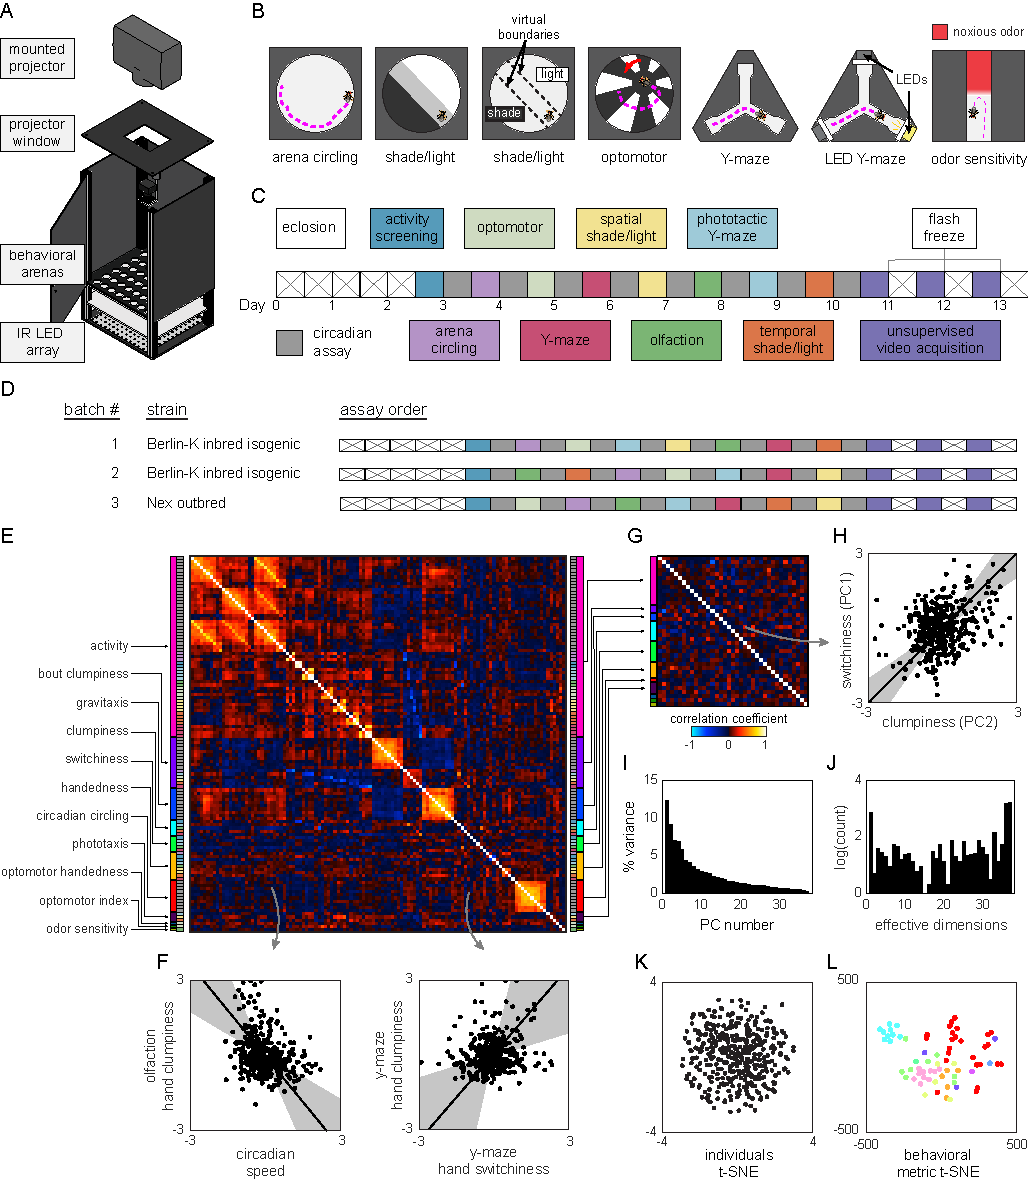
\includegraphics[width=\textwidth]{../figures/chapter_3/fig_3-1.pdf}
    \vspace{.1in}
    \caption*{Figure 3.1 — Decathlon experimental design. A) Schematic of the imaging rig used for most Decathlon experiments. B) Schematics of the behavioral assays, illustrating the geometry of the arenas and stimulus structure. C) Timeline of the Decathlon experiment. Colors indicate the assays conducted on each day, half-black half-white blocks indicate the circadian assay and storage in 96-well plates. D) Timelines of the three Decathlon experiments, indicating the randomized order of assays 2-8.}
\end{figure}

In order to obtain all of the behavior measures from each experimental animal, we put the assays together in a serial experimental pipeline lasting 13 consecutive days (Figure 3.1c), generally with one unique assay per day and continuous circadian imaging (assay 9) between assays. This pipeline begins with 3 day-old flies being loaded into the 96-well circadian imaging plates. The flies acclimatized to these chambers over two days. Starting on day 3, daily assays began, and on each day, flies were lightly anesthetized on a ice-chilled plate and aspirated, maintaining their identity, into the assay arrays. After the assay was completed (typically after 2h of recording) flies were again lightly anesthetized and returned to 96-well plates for renewed circadian imaging. On the first such day, flies were loaded into an array of circular arenas and imaged for total activity (in a version of assay 1). At this point, the most active 192 flies were retained for further testing. In preliminary experiments, we found that flies that were inactive at the beginning of the pipeline were very unlikely to produce substantial amounts of data over the rest of the pipeline. With the addition of this activity-screening assay, the total number of experiments was 10, and as each fly “competes” in all 10 events, we refer to the entire pipeline as a Decathlon. 

It is possible that the assay order has some effect on the recorded behavior measures. So we randomized the assay order between Decathlon implementations as much as possible (Figure 3.1d), subject to two restrictions: activity-screening was always the first assay, and high-resolution imaging for unsupervised analysis (assay 8) was always the last assay. (This assay has lower throughput, and three days were required to complete all 168 remaining flies. If this assay were performed earlier in the pipeline, it might introduce heterogeneity across subsequent assays.) When each fly completed its run through all Decathlon assays (i.e., over the three days of assay 8 imaging), it was flash-frozen in liquid nitrogen for RNA sequencing. 

To collect data that would reveal the structure of behavioral variation within a genotype, we conducted two Decathlons using highly inbred, nearly isogenic flies derived from the wild type strain Berlin-K (BSC#8522, \cite{Nothel_1981}. We confirmed that this strain was, indeed, highly isogenic with genomic sequencing of individual animals, finding ~75 SNPs in the population across the entire genome (figure S2). 115 flies completed the first Decathlon, and 176 the second. While we aimed to collect 121 measures per fly, a portion of values were missing, typically because flies did not meet assay-specific activity cutoffs. For subsequent analyses (See figure S3 for a schematic of all analysis pipelines), it was sometimes necessary to have a complete data matrix. So we infilled missing values using the alternating least squares method, which, as judged by analyses of toy ground-truthed data, performed better than mean-infilling (figure S4). We wanted, for the sake of maximal statistical power, to merge the data sets from the two Berlin-K\textsuperscript{iso} Decathlons. The correlation matrices of these two data sets were not identical, but were substantially more similar than expected by chance (figure S5), implying that while there were inter-Decathlon effects, much of the same structure was present in each, and merging them justified. To do this, we z-score normalized the data points from each arena array/batch (within each Decathlon) across flies, thus eliminating any arena, assay, and Decathlon effects and enriching the data for contrasts between individuals. A grand data matrix was made by concatenating these batches (382 individuals x 121 behavior measures).

The full correlation matrix of this Berlin-K\textsuperscript{iso} data set is shown in figure 3.2a. It contains a substantial amount of structure, indicating that large groups of behavioral measures covary. But the covariance of many pairs of measures in the matrix is not surprising. For example, almost all our assays generate some measure of locomotor activity (meanSpeed in circular arenas, number of turns in Y-mazes, meanSpeed in the olfactory tunnels, etc.), and one might expect that especially active flies in one assay will be especially active in another assay. Additional unsurprising structure in this matrix comes identical measures recorded in each of the 11-13 circadian assays each fly completed. But, even in this first analysis, surprising correlations were evident. For example, flies with higher variation in the inter-turn interval in the olfactory assay (olfactoryTurnClumpiness) exhibited higher mean speed in the circadian assays, and flies with higher variation in inter-turn intervals in the Y-maze (ymazeTurnClumpiness) exhibited lower mutual information in the direction of subsequent turns in the Y-maze (ymazeHandSwitchiness) (figure 3.2b). See Buchanan et al., 2015, and Akhund-Zade et al., 2019 for more about these measures.

\begin{figure}[t!]
    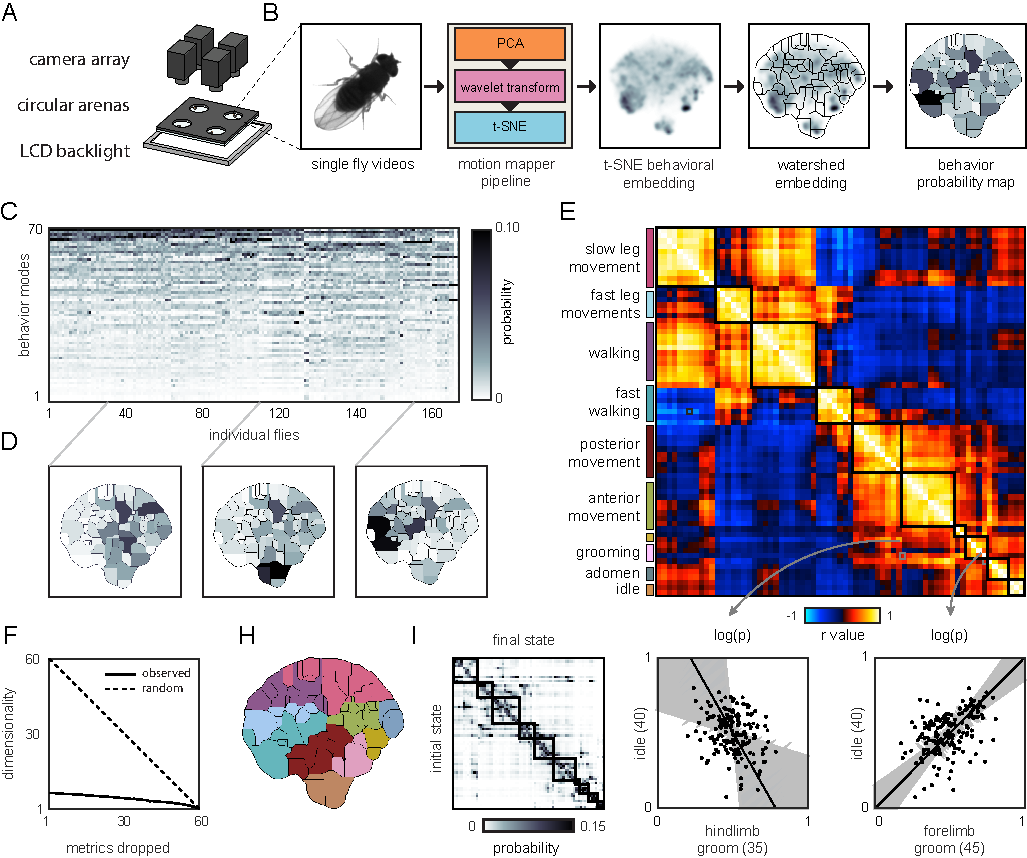
\includegraphics[width=\textwidth]{../figures/chapter_3/fig_3-2.pdf}
    \caption{Figure 3.2 — Decathlon behavioral variation. A) Full correlation matrix of all raw behavioral measures taken in the Decathlon. Colored blocks indicate blocks of measures we thought a priori might be correlated (outer blocks, text labels). Inner blocks indicate assay. B) Example scatter plots associated with measure correlations. Points are individual flies. Line is the best fit (PC1 of these points), grey region is the 95\% confidence interval of the fit, as determined by bootstrap resampling. C) Distilled correlation matrix in which all correlated metrics represent unexpected relationships. D) Example scatter plot from the distilled correlations. Plot elements as in B. E) Scree plot of the ranked, normalized eigenvalues, i.e., the \% variance explained by each PC, of the distilled behavior matrix, versus PC #. F) Effective dimensionality spectrum (See text and Figure S9) for the distilled matrix. Height of bars indicates organization at that dimensionality. G) Points corresponding to individual flies non-linearly embedded using t-sne from the 121-dimensional raw measure space to two dimensions. H) Points corresponding to behavioral measures non-linearly embedded using t-sne from the 384-dimensional space of flies to two dimensions. Colors indicate groups of measures we expected a priori to be related.}
\end{figure}

To produce an exhaustive list of such “interesting” correlations, we distilled the grand correlation matrix to a smaller matrix (the “distilled matrix”; figure 3.2c) in which two kinds of interesting relationships were revealed: 1) uncorrrelated dimensions among measures for which we had a prior expectation of correlation (e.g., if meanSpeed in circular arenas is found to be uncorrelated with meanSpeed in olfactory tunnels), and 2) correlated dimensions among measures for which we had no prior expectation of correlation. Relationships of the former class were identified by enumerating, before we ran any correlation analyses, groups of measures we expected to be correlated (“a priori groups”; figure 3.2a,h). We looked for surprising independence within such groups by computing the principal components of data submatrices defined by the grouping (e.g. for the “activity” a priori group, by running PCA on the data set consisting of 382 individual flies, and 57 nominal measures of activity). We then replaced each a priori group submatrix with its projection onto its statistically significant PCs, as determined by a reshuffling analysis (see Methods, figure S7). Some a priori groups largely matched our expectations, with relatively few independent dimensions among many measures (e.g., the gravitaxis group which had 10 measures and only 2 significant PCs), while others exhibited relatively many independent dimensions (e.g., the clumpiness group which had 5 measures and 5 significant PCs; see figure S7 for all a priori group PCA analyses). 

With a priori group submatrices represented in their respective significant PCs, the grand data matrix now contained 38 behavioral metrics. Every significant correlation between behavioral metrics at this point represents an unexpected element of structure of behavioral variation (figure 3.2c). The first impression of this correlation matrix is that it is sparse. Most behavioral metrics are uncorrelated or weakly correlated, meaning there are many independent dimensions of behavioral variation. However, 176 pairs of behaviors were significantly correlated at a false discovery rate of 38.1\%, and the distribution of p-values for the entries in this matrix exhibits a clear enrichment of low values (figure S7) indicating an enrichment of significant correlations. As an example, flies with high values in the third PC of the switchiness a priori group tend to have high values in the second PC of the clumpiness a priori group (figure 3.2d; a relationship that is built, in part, on the positive correlation between the ymazeTurnClumpiness and ymazeHandSwitchiness, figure 3.2d). Interpreting the loadings (figure S7) of these PCs indicates that this is a correlation between olfactory tunnel turn direction switchiness and olfactory tunnel turn timing clumpiness. We detected a substantial number of correlations between different dimensions of switchiness and clumpiness (figure S8), suggesting there are multiple couplings between these suites of traits. 

Stepping back from specific pairwise correlations, we examined the overall geometry of behavioral variation. The full matrix contained 22 significant PCs, with PCs1-3 explaining 9.30, 6.94 and 5.77 \% of the variance, respectively (figure 3.2e). But amount of variance explained across PCs does not indicate how many independent dimensions of variation are present in a data set. Moreover, a correlation matrix can be organized at different scales/hierarchically, so there need not be a single number that characterizes effective dimensionality. We developed an “effective dimensionality spectral analysis” that assessed the continuous degree of organization of a data set across the continuous range of dimensionalities from 1 to d, the dimensionality of the data. Briefly, we thresholded the correlation matrix, across a wide range of thresholds, at each identifying the number of connected components in the matrix and recorded how often n connected components were observed. See Methods and figure S9. The effective dimension spectrum (figure 3.2f) of the distilled Decathlon data set had peaks at 1 and d (37). There was also evidence for structure over the full range of intermediate dimensionalities. Overall, the organization appears to be predominantly independent behaviors, with some sparse sets of genes correlated with varying strengths. 

To assess how individual flies are distributed in behavior space, we embedded them from the 384 dimensional space into two dimensions using t-sne \cite{Maaten_Visualizing_2008}. There appear to be no discrete clusters corresponding to “types” of flies, instead, variation among flies appears continuously distributed around a single mode (figure 3.2g). We also embedded behavioral metrics as points from the 121 dimensional space of flies into two dimensions (figure 3.2h). This confirmed that while our intuition for which sets of metrics would be similar (the a priori groups) was right in many cases, metrics we thought would be similar were often dissimilar across flies, and sometimes metrics we did not anticipate being similar were (e.g., phototaxis and activity level). 

With data from the second Decathlon, we characterized the structure of variation in a set of behaviors that was potentially exhaustive for one behavioral condition (free walking/motion in a 2d arena; figure 3.3a). High-speed, high-resolution video was acquired for four flies simultaneously in each of two rigs. Over three days, we acquired 13.5 GB of 200x200 px 100Hz videos centered on each fly as they behaved spontaneously over the course of 60 minutes. These frames were fed into an unsupervised analysis pipeline \cite{berman_choi_bialek_shaevitz_2014} that computed high-dimensional representations of these data in the time-frequency domain before embedding them in two dimensions and demarcating boundaries between 70 discrete modes of behavior (figure 3.3b). The behavior of each fly was thus represented as one of 70 values at each frame. Flies exhibited a broadly similar probability distribution of performing each of these behaviors (figure 3.3c), though there were conspicuous differences among individual patterns of behavior (figure 3.3d).

\begin{figure}[t!]
    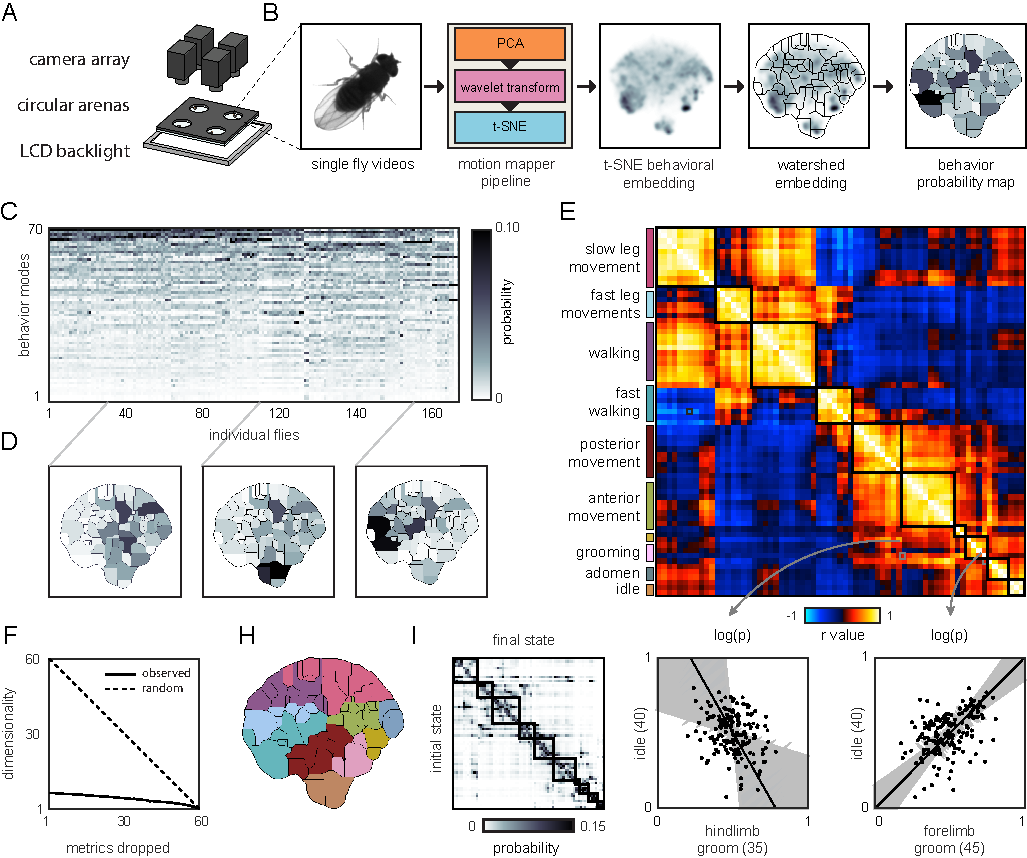
\includegraphics[width=\textwidth]{../figures/chapter_3/fig_3-3.pdf}
    \vspace{.1in}
    \caption*{Figure 3.3 — Correlation structure of unsupervised behavioral classifications. A) Schematic of the four camera imaging rig used to acquire single fly videos. B) Overview of the data processing pipeline from single fly videos to behavioral probability maps. C) Behavioral classification probability density function (PDF) matrix. Columns correspond to behavioral PDFs for individual flies. D) Sample individual PDFs mapped to locations in tSNE space. Discrete regions correspond to watersheds of the tSNE embedded probability densities. E) Correlation matrix (top) for individual PDFs with rows and columns hierarchical clustered. Colored blocks indicate supervised labels applied to classifications post-hoc. Example scatter plots (bottom) of individual behavioral probabilities. Points correspond to probabilities for individual flies. Line is the best fit (PC1 of these points), grey region is the 95\% confidence interval of the fit, as determined by bootstrap resampling. F) Effective dimensionality of the unsupervised behavioral classifications as calculated by the scree plot intersection of the observed and shuffled PDF matrices (see methods). H)  Discrete behavioral map with individuals zones colored by supervised labels as in E. I) Transition probability matrix for behavioral classifications. Entries in the ith row and jth column correspond to the probability of transitioning from state i to state j. Blocks on the diagonal indicate clusters of supervised labels is in E.}
\end{figure}

The correlation matrix of behavioral modes identified in the unsupervised analysis was highly structured (figure 3.3e; like the correlation matrix of the rest of the decathlon metrics, figure 3.1e), appearing to have approximately 6 independent dimensions of variation (figure 3.3f). For this analysis, there was no equivalent of a priori groups of behavioral measures, as metrics were not defined prior to the analysis. But, in examining sample movies of flies executing each of the 70 unsupervised behavioral modes, it was clear that highly correlated behavioral modes tended to reflect variations on the same type of behavior (e.g., walking) or behaviors performed on the same region of the body (e.g., anterior movements including eye and foreleg grooming; figure 3.3g). In other words, individual flies that perform more eye grooming tend to perform more of other anterior behaviors. There were some correlations between seemingly disparate behaviors. For example, flies that spent more time performing REFREF anterior grooming also spent more time performing REFREF slow leg movements (figure 3.3g). The overall similarity of covarying behaviors was confirmed by defining groups of covarying behaviors and observing that they were associated with contiguous regions of the embedded behavioral map (figure 3.3i). That is, behaviors whose prevalence covaries across individuals have similar time-frequency patterns across the body. Moreover, these clusters of covarying, contiguously embedded behaviors exhibited similar temporal transitions; behaviors that covary across individuals tend to precede specific sets of subsequent behaviors (figure 3.3j). Thus, there appear to be couplings between the dimensions of behavioral variation across individuals, the domains of the body implementing behavior, and the temporal patterning of behaviors. 

To confirm that the Decathlon experiments revealed biologically meaningful couplings between behaviors, we treated correlations in the Decathlon matrices as hypotheses to test in a thermogenetic neural circuit perturbation screen. Specifically, we focused on the many correlations between measures of turn timing clumpiness and turn direction switchiness (figures 3.1e, S8). Before the Decathlon experiment, we had no reason to think these measures would be correlated as one describes higher order structure in the timing of locomotor turns (clumpiness) and one describes higher order structure in the direction of sequential turns (switchiness). Our Decathlon-derived prediction was that if perturbing a circuit element caused a change in clumpiness, it would tend to also cause a change in switchiness, in a consistent direction.  We looked for such correlated changes when we inactivated or activated neurons in the Central Complex, a cluster of neuropils involved in locomotor behaviors \cite{Buchanan_Neuronal_2015,Ofstad_Visual_2011,Kottler_Inverse_2019} and heading estimation \cite{Seelig_Neural_2015,green_nature_2017,Kakaria_Ring_2017}. We used a set of Gal4 lines \cite{Wolff_Neuroarchitecture_2018}, each of which targets a single cell type and that tile the entire Protocerebral Bridge (a Central Complex neuropil) (See Table 1), to express Shibirets \cite{of_neurobiology_Conditional_2001} or dTRPA1 \cite{Hamada_An_2008}, thermogenetic reagents that block vesicular release and depolarize cells respectively. As controls, we used flies heterozygous for the Gal4 lines, and lacking the effector transgenes. 

Flies with these genotypes were loaded into Y-mazes for behavior imaging before, during and after a temperature ramp from 23°C to 29°C (figure 3.4a). At the permissive temperature, we observed no correlation in the average line clumpiness and switchiness (figure 3.4b,d). This suggests that the mechanisms which couple variation in switchiness and clumpiness within a genotype may not be at play across genotypes. In contrast, at the restrictive temperature, we saw significant correlations between clumpiness and switchiness in all three experimental treatments: control, Shibirets and dTRPA1 lines (figure 3 .2c,d). That this correlation appeared in controls suggests that temperature alone can selectively alter the function of circuit elements regulating both clumpiness and switchiness. The strongest correlation at the restrictive temperature was seen in the dTRPA1 lines, indicating that activating specific circuit elements can produce correlated effects on clumpiness and switchiness. While clumpiness and switchiness changed dramatically in some lines (table 3.2), the pattern of stronger correlations between these measures at the restrictive temperature, especially in lines expressing dTRPA1 in neural circuit elements, was consistent in the lines where changes were more modest (figure 3.4c, bottom).

\begin{figure}[t!]
    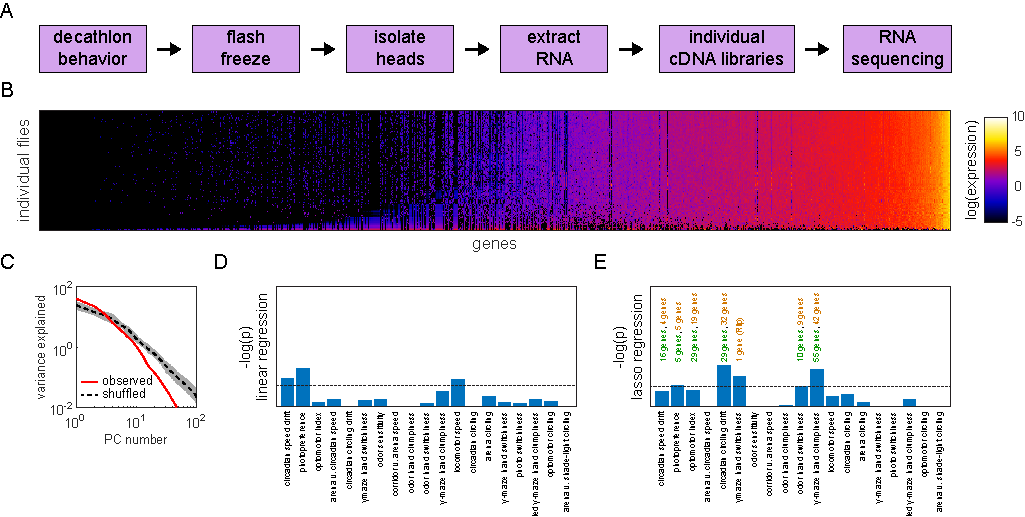
\includegraphics[width=\textwidth]{../figures/chapter_3/fig_3-4.pdf}
    \vspace{.1in}
    \caption*{Figure 3.4 — Effect of thermogenetic neural perturbation on clumpiness and switchiness. A) Schematic overview of the screen genetic crosses (left) and behavioral paradigm (right). Plot depicts the schema used to activate or silence neurons. Colored hash marks indicate periods when the light was on (cyan) or off (red). B) Diagram of the various neurons (solid lines) target by lines tested in the screen. C) Scatter plots of line average clumpiness and switchiness at the permissive (left) and restrictive (right) temperatures. Plots on the top row include all lines screened. Plots bottom row  exclude the 8 lines with the lowest clumpiness and switchiness measures at the restrictive temperature. Lines indicate the line of best fit and shaded regions indicate the 95\% confidence of the fit as determined by bootstrap resampling. D) Correlation coefficients for each effector type at the permissive and restrictive temperatures for all lines (top) and a subset of lines (bottom) as in C. Error bars indicate the 95\% confidence interval as determined by bootstrap resampling.}
\end{figure}

That thermogenetic manipulation can cause correlated changes in behavioral measures, suggests that stochastic intragenotypic variation in neural physiology might account for correlated variation in measures in wild type flies. Such physiological variation could arise in stochastic variation in gene expression \cite{Lin_Microenvironmental_2016} in circuit elements. To test this hypothesis, we performed RNA sequencing on the heads of the flies at the end of the first Decathlon experiment (figure 3.5a). We used Tm3’seq \cite{Pallares_TM3_2019} to make 3’-biased libraries for each individual animal. We quantified the expression of 17,470 genes in 48 flies. The expression profiles were strongly correlated across individuals (figure 3.5b), but there was some evident variation across individuals (figure 3.5c). To assess whether this variation was meaningful with respect to behavioral variation, we trained two kinds of models to predict individual behavioral biases from individual patterns of gene expression. The first of these examined whether an individual’s position on the major axes of transcriptomic variation predicted its behavioral biases. Specifically, we fit linear models to predict flies’ values on the principal components of the distilled behavioral matrix from their values on the first REFREF principal components of transcriptomic variation. Cross-validated models were significantly predictive for 3 different behavioral components (figure 3.5d), including locomotor speed and phototactic preference. The second model assessed whether specific genes or small sets of genes predicted behavioral biases. We specifically used lasso regression \cite{Santosa_Linear_1986,of_the_B_Regression_1996} to identify sparse gene predictors of individual bias on the PCs of the distilled matrix. As in the other analysis, cross-validated models were significantly predictive for some behavioral biases (figure 3.5e). Of the behavioral metrics that could be predicted from the transcriptomic data, most were only predictable using one of these approaches. 

\begin{figure}[t!]
    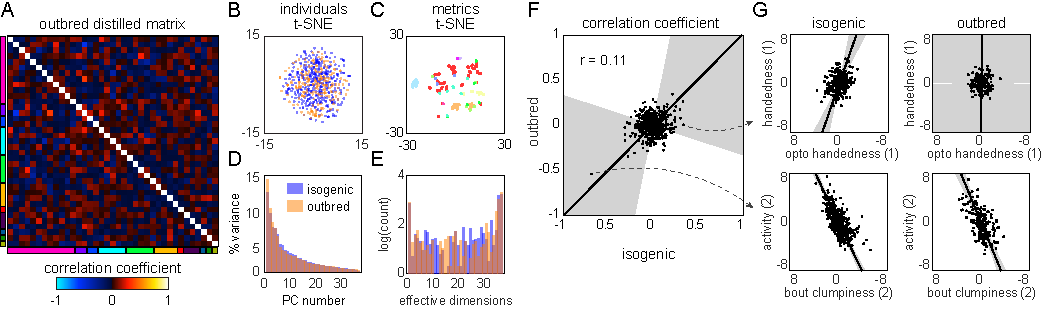
\includegraphics[width=\textwidth]{../figures/chapter_3/fig_3-5.pdf}
    \vspace{.05in}
    \caption*{\textbf{Figure 3.5} — Gene expression profiling of decathlon flies.}
\end{figure}

If transcriptomic differences predict individual behavioral differences within a genotype, then the structure of behavioral variability might be very different in outbred populations, where transcriptomic differences are (presumably) much more substantial. We tested this by conducting a Decathlon experiment on outbred flies from a synthetic genetic mapping population \cite{Long_Dissecting_2014}. These animals were from a high (~100)-generation intercross population (“NEX”; seeded in the first generation by eight kinds of F1 heterozygotes produced by round-robin cross from eight inbred wild strains). A distilled correlation matrix of behavior metrics (figure 3.6a) was produced by the same method as above. At first glance, it appears qualitatively similar to the distilled correlation matrix from isogenic animals (figure 3.1e). This impression was confirmed in more formal comparisons of the structure of behavior in inbred and outbred populations. In isogenic and outbred populations: 1) individuals do not fall into discrete clusters, as determined by t-sne embedding of individuals as points (figure 3.6b, left). Moreover inbred and outbred flies appear to lie on the same manifold in behavior metric space; 2) behavioral measures cluster according to their membership in a priori groups similarly in outbred (figure 3.6b, right) and inbred (figure 3.1k) populations; 3) the distribution of \% variance explained by principal component was similar (figure 3.6c, left); and 4) there is a similar spectrum of covariance structure, with most metrics independent, and a sparse network of correlations of varying strength (figure 3.6c, right). 

After determining that the overall structure of behavioral variation in isogenic and outbred populations is similar, we asked whether it was also similar in specific correlations. There appears to be some similarity at this level (figure 3.6d); the correlation coefficient between the isogenic and outbred populations in the pairwise correlations between behavior metrics is statistically significant (p = 0.001), but low in magnitude (r = 0.12). Examining specific pairs of behavior metric scatter plots, the range of consistency and inconsistency in the correlation relationships between the isogenic and outbred experiments is clear (figure 3.6e). A caveat in interpreting apparent differences between the isogenic and outbred matrices is that two qualities are different between the animals used in the respective experiments: the degree of genetic diversity, but also (necessarily) the genetic background of the flies.

\begin{figure}[t!]
    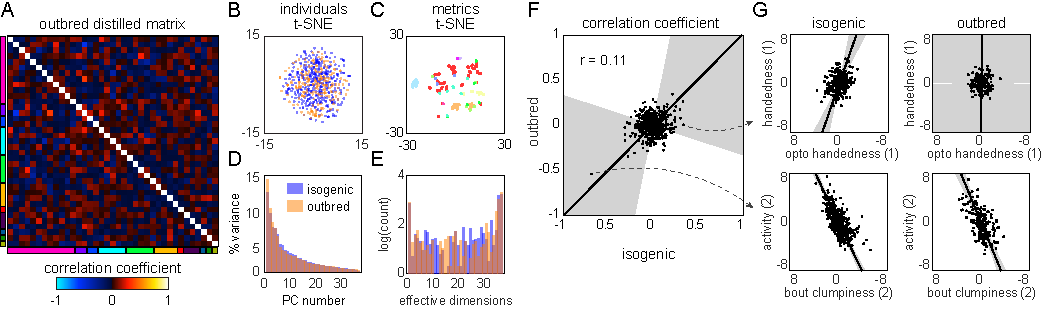
\includegraphics[width=\textwidth]{../figures/chapter_3/fig_3-6.pdf}
    \vspace{.05in}
    \caption*{\textbf{Figure 3.6} — Structure of behavioral variation in outbred flies. A) Distilled correlation matrix for outbred NEX flies. Colored blocks indicate a priori groups as described in figure 1. B) Points corresponding to individual flies non-linearly embedded using t-sne from the 121-dimensional raw measure space to two dimensions. Color indicates whether the genotype is isogenic (blue) or outbred (orange). C) Points corresponding to behavioral measures non-linearly embedded using t-sne from the 192-dimensional space of flies to two dimensions. Colors correspond to a priori group. D) Scree plot of the ranked, normalized eigenvalues, i.e., the \% variance explained by each PC, of the distilled covariance matrix, versus PC #. E) Log histogram of the effective dimensionality of the distilled matrix, as calculated by the number of connected components in the thresholded graph covariance matrix over 5,000 linearly spaced covariance thresholds (see methods). F) Scatter plot of the distilled matrix correlation coefficients for isogenic and outbred flies. Points correspond to distilled matrix metric pairs. G) Example scatter plots of distilled matrix metric pairs for inbred (left) and outbred (right) flies. The rows of plots highlight a pair of metrics with qualitatively different (top) and similar (bottom) correlations in inbred and outbred flies.}
\end{figure}

Lastly, we examined how the correlation structure of behavior compared between sets of flies with variation coming from different sources. Specifically, we looked at four data sets: 1) the BABAM data set \cite{Robie_Mapping_2017} in which measures were acquired from groups of flies behaving in open arenas, and variation came from the thermogenetic activation of 2,381 different sets of neurons (the first generation FlyLight Gal4 lines \cite{Jenett_A_2012}); 2) a Drosophila Genome Reference Panel (DGRP; \cite{Mackay_The_2012}) behavioral data set, in which measures were acquired in behavioral assays similar to the Decathlon experiments (sometimes manually, sometimes automatically) and variation came from the natural genetic variation between lines in the DGRP collection; 3) a DGRP physiological data set, in which measures are physiological or metabolic (e.g., REFREF) and variation came from the natural genetic variation between lines in the DGRP collection; and 4) the split-Gal4 Descending Neuron (DN) data set \cite{Cande_Optogenetic_2018} in which measures came from the same unsupervised cluster approach as figure 3.3, and variation comes from the optogenetic activation of specific sets of descending neurons projecting from the brain to the ventral nerve cord (\cite{Namiki_The_2018}). We analyzed these data sets with the same tools we used to characterize the structure of behavioral variation in the Decathlon experiments.

\begin{figure}[t!]
    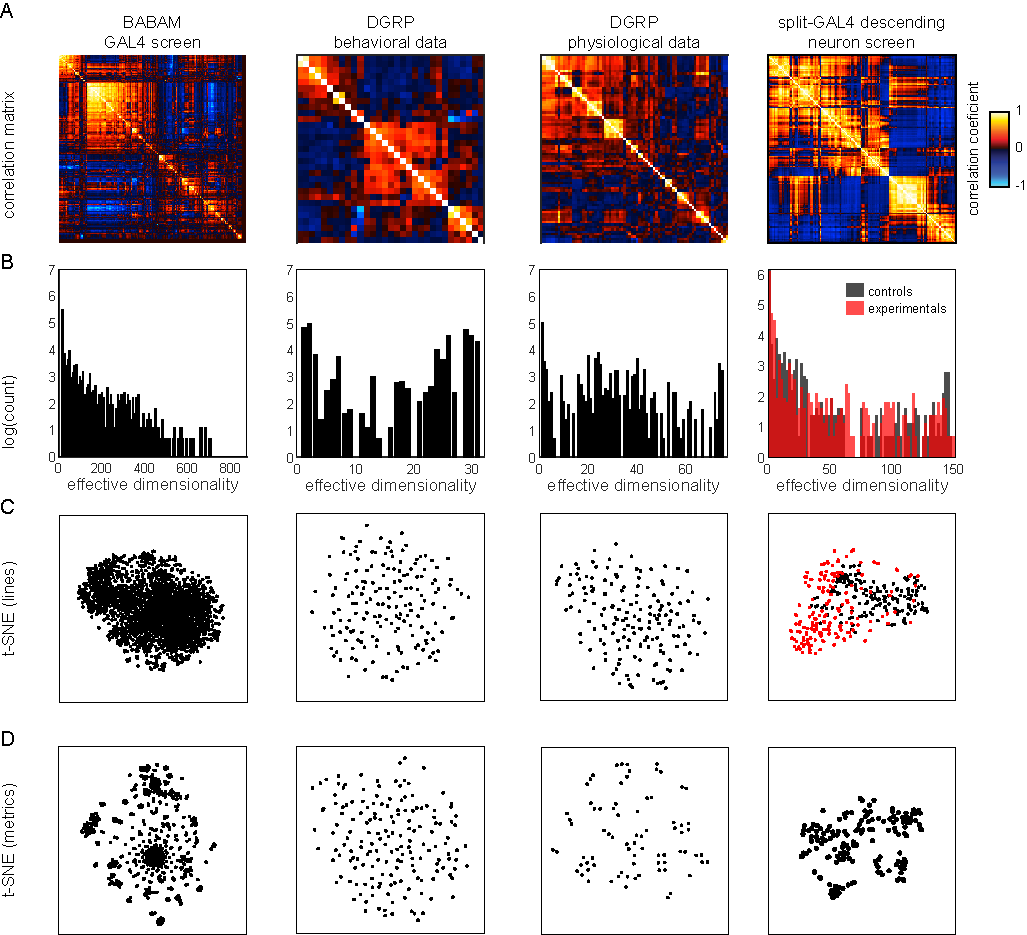
\includegraphics[width=\textwidth]{../figures/chapter_3/fig_3-7.pdf}
    \vspace{.05in}
    \caption*{\textbf{Figure 3.7} — Meta analysis of drosophila covariation. A) Correlation matrices of previously published data sets. Columns correspond to analyses performed on each data set. From left to right, the data sets are as follows: line averages of supervised behavioral classifications following thermogenetic inactivation in the fly olympiad screen \cite{Robie_Mapping_2017}, line averages of behavioral phenotypic data from wild-type inbred lines in the Drosophila genomic reference panel (DGRP) database \cite{Mackay_The_2012}, line averages of physiological phenotypic data from the DGRP database, line averages of the fold change in unsupervised behavioral classifications following optogenetic activation of descending neurons \cite{Cande_Optogenetic_2018}. B) Log histograms of the effective dimensionality of all data sets, as calculated by the number of connected components in the thresholded graph covariance matrix over 1,000 linearly spaced covariance thresholds (see methods). Color in the rightmost plots (B-D) indicates either control (Gal4 driver only) or experimental animals (Gal4 x dTrapA1). C) Points corresponding to lines non-linearly embedded using t-SNE from the D-dimensional raw measure space to two dimensions (from left to right, D = 871, 31, 77, 151). D) Points corresponding to lines non-linearly embedded using t-SNE from the N-dimensional raw measure space to two dimensions (from left to right, N = 2083, 169, 169, 176).}
\end{figure}

All of these data sets show substantial structure in their correlation matrices (figure 3.7a, S10). The BABAM and especially the DN correlation matrices contain numerous high correlation values, indicative of strong couplings between behaviors under these neuronal manipulations. The DGRP correlation matrices, especially the DGRP behavioral matrix, look more qualitatively similar to the Decathlon matrix, with lower, sparser correlations. This suggests that behavioral variation has coarsely similar structure whether variation arises intragenotypically (e.g., through stochastic variation in transcription [figure 3.5b]; figure 3.1g), intergenotypically among outbred individuals (figure 3.6a), or intergenotypically among inbred lines derived from wild populations (figure 3.7a). A caveat of this conclusion is that sparse correlation matrices can arise either from true, biological independence of behavior measures or from measurement error. The effective dimensionality spectra of these matrices largely recapitulate the similarity of the DGRP behavior and Decathlon structures (figure 3.7b). The BABAM and DN spectra peak at 1, suggesting that most measures are in a single network of couplings to other measures. This is especially true in the BABAM data, and more true in the optogenetic experimental animals than controls in the DN data. The DGRP physiology data exhibits peaks at dimensionality 1 and d, but also a broad peak between 20 and 40, suggesting that intergenotypic variation in physiology may have an intrinsic dimensionality in that range. The spectrum of the DGRP behavior data looks similar to that of the Decathlons, with peaks and 1 and d, and evidence for structure over the full range of intermediate dimensionalities. The distribution of individual lines in the space of DGRP behavior (and physiology) measures appears to be distributed single mode (figure 3.7c), like individual flies in the Decathlon (figure 3.1j). In contrast, there is some organization of individual lines in the BABAM and DN data sets, likely reflecting neuronal perturbations affecting multiple circuit elements mediating the same behavior(s), e.g., multiple lines targeting the same neuropil. Measures fall into clusters in all of these data sets except the DGRP behavior measures (figure 3.7d), which appear distributed around a single mode, perhaps reflecting the high dimensionality of behavior itself. 


Discussion

Individuals exhibit different behaviors, even when they have the same genotype and have been reared in the same environment. These differences might co-vary, or lie on a manifold of specific geometry in behavior variation-space, but the structure of intragenotypic behavioral variation is uncharacterized. We designed a pipeline of ten behavioral assays (figure 3.1) which collectively yielded up to 121 behavioral measures per individual animal. We also used unsupervised clustering to identify an additional 70 measures per individual based on a time-frequencing analysis of high resolution video of the flies behaving spontaneously (figure 3.3). These measures were the fly-specific rates of exhibiting each of the 70 unsupervised behavioral modes. All in all, across three 15 day Decathlon experiments, we collected 191 behavior measures from 576 flies. This allowed us to produce a full correlation matrix for all the behavioral measures for the variation present in isogenic animals grown in the lab (figure 3.1e). 

This is significant for quantitative geneticists because this matrix (with a little algebraic manipulation) is a direct measurement of the Permanent Environment variance-covariance matrix, one of the major components of the Phenotypic variance-covariance matrix along with the famous G-matrix \cite{Charmantier_Quantitative_2014}. Meta-analysis of behavioral traits that have been assessed for their genetic variance-covariance indicates that across behaviors, ~23\% of variance can be attributed to heritable factors \cite{Dochtermann_The_2019}. This means that “environmental” factors, which include intragenotypic individual behaviors like the ones we measured here, explain ~77\% of behavioral variance. So characterizing the structure of Permanent Environment variance-covariance will contribute to closing a significant gap in our understanding of the basis of behavioral diversity.

For ethologists and behavioral neuroscientists, this result represents the most complete characterization of the geometry of behavioral variation, which can be thought of as emergent product of developmental biological processes and the dynamic interaction of neural activity and animals’ environment. From the full behavioral matrix we made a so-called “distilled” matrix in which any significant correlation indicates a surprising new relation between behaviors (figure3.1g and S8). This form of the data minimizes duplicated measures of the same behavior, allow us to cleanly analyze the geometry of behavioral variation. We found that behavioral measures were largely independent of each other, so that the main effective dimensionality of the behavioral space matched the number of behaviors measured. But a single number cannot fully characterize the dimensional organization of a correlation matrix, so we developed a spectral approach that examined the degree of organization across all possible dimensionalities in the data (figure 3.1j, 3.3e, 3.6b, S10). This revealed a degree of organization at intermediate dimensionality corresponding to sparse correlations between specific pairs of behaviors (figure 3.1g,h, S9). We found no evidence of discrete types of flies. Embedding data points corresponding to individual flies from the high dimensional space of individual biases into two dimensions produced a broad distribution around a single mode (figure 3.1j).

One the specific, surprising correlations we discovered was between “clumpiness” and “switchiness” (figures 3.1f,h, 3.3, S8). These are slightly abstract, higher-order behavior measures, corresponding respectively to the burstiness of turn/action/decision timing and the degree of independence between consecutive binary choices. We had no a priori reason to expect these measures would be correlated, since one pertains to the structure of actions in time, and one pertains to the persistence of trial-to-trial biases. The correlation between these two behaviors (or other pairs we discovered) could be established during development. Individual wiring \cite{Linneweber_A_2019,Mellert_Genetic_2016} or physiological variations in neurons that mediate more than one behavior could impart coupled changes to all such behaviors. 

If such an explanation accounts for the correlation of clumpiness and switchiness, there may be shared neural circuit elements in the circuits controlling decision-timing and decision-bias. We tested this idea in a thermogenetic screen of circuit elements in the central complex, a brain region where heading-direction is represented \cite{Seelig_Neural_2015} in a ring-attractor circuit \cite{Kakaria_Ring_2017}. We found that when a thermogenetic manipulation affected clumpiness, it tended to also affect switchiness (figure 3.4), consistent with the prediction of shared circuit elements. Interestingly, we also found that the effector-inducing temperature manipulation alone concomitantly changed clumpiness and switchiness in some lines. This suggests that potentially subtle alterations of circuit physiology (e.g., temperature shifts [\cite{Haddad_Circuit_2018}] well within physiological limits) can affect the function of circuit elements governing multiple behaviors. 

We included behavioral assays in the Decathlon pipeline under a number of constraints. They assays had to be high throughput, both in the number of flies that could be assayed and in measures being automatically acquired. Flies had to survive at high rates, and the measures had to be stable over multiple days (figure S1), because the whole experiment lasted 15 days. Because not all behavior measures showed robust stability for this duration (all showed at least some day-to-day stability), the distilled Decathlon matrices likely represent an underestimate of the behavioral couplings exhibited over short periods (and perhaps an overestimate of life-long couplings, as flies can live more than a month; \cite{Linford_Measurement_2013}). In the end, we employed a number of spontaneous locomotion assays and simple stimulus-evoked assays like odor-avoidance and phototaxis. 

Light responses were measured in a number of assays (Table S1), specifically: the LED Y-maze \cite{Werkhoven_MARGO_2019} (in which flies turned toward or away from lit LEDs in a rapid trial-by-trial format), the Spatial Shade-Light assay (in which flies chose to stand in lit or shaded regions of an arena that only changed every 4 minutes), and Temporal Shade-Light (in which the same luminance levels were used as the previous assay, but a fly experienced them by traveling into virtual zones which triggered the illumination of the whole arena at a particular luminance) ) (figure 3.1b). These assays were potentially redundant, and we included this cluster of phototaxis assays in part as a positive control. However, the three phototactic measures we thought would be correlated a priori were, in fact, independent of each other, each being represented in the distilled correlation matrix (figure 3.1g). This may reflect flies using different behavioral algorithms \cite{Krakauer_Neuroscience_2017}, implemented by non-overlapping circuits, to implement these behaviors. Indeed, independence between behavior measure was the typical observation. This also suggests that we have not come close to sampling the full dimensionality of intragenotypic behavioral variation; if we were able to add more measurements to the experiment, they too would likely be independent.

To address potential biases in our sampling of assay and measure space, we performed an unsupervised analysis \cite{berman_choi_bialek_shaevitz_2014,Cande_Optogenetic_2018}, of flies walking spontaneously in arenas. This approach has the potential to identify all the modes of behavior exhibited in that context. Moreover, because the unsupervised algorithm is fundamentally a clustering algorithm, it does not necessarily return a definitive number of clusters/behavioral modes (with more data, it can find increasingly more clusters). Because we can also extract second-order behavioral measures from this approach, such as Markov-transition rates between modes, this approach has the potential to yield a huge number of measures. In the end we were conservative in the number of measurements we chose to work with, matching it to the same order of magnitude as the number of flies we tested. The correlation matrix for the unsupervised behavior measures featured stronger correlations than the distilled Decathlon matrices (figure 3.3e). Yet it had a similar effective dimensionality spectrum, indicating many independent dimensions of variation and that not all behavior modes had been sampled (figure 3.3f). 

Interestingly, the blocks of structure in the correlation matrix aligned, to some extent, with the blocks of structure in the Markov transition matrix of these behavioral measures. This suggests that behaviors mediated by non-overlapping circuits (those that vary independently across individuals) more rarely transition to each other over time. Conversely, behaviors mediated by overlapping circuitry are likely to follow each other sequentially. This may reflect the influence internal states \cite{Calhoun_Unsupervised_2019}, with an internal state jointly determining what subset of overlapping neurons drives behaviors that are appropriate to string together in succession \cite{Seeds_A_2014}. We did not assess the day-to-day persistence of behavioral modes identified in the unsupervised analysis, so the observed variation across flies could reflect moods rather than permanent personalities. However, previous supervised \cite{Kain_Leg_2013} and unsupervised \cite{Todd_Systematic_2017} analyses of spontaneous microbehaviors similar to those identified by unsupervised approaches have found such behaviors to persist across days.

We investigated whether individual variation in transcript abundance would predict individual biases on the axes of intragenotypic variation. At the end of the Decathlon, flies were flash frozen and their heads were RNA sequenced. We fit two kinds of model with this data (figure 3.5). First, a linear model was used to predict behavioral biases on the axes of the distilled data set using principal components of transcript variation as independent variables. Second, lasso-regularized regression was used to predict the same behaviors scores using individual gene abundances. Both of these modeling approaches succeeded in predicting some behavior scores. Linear models successfully predicted changes in mean speed over the circadian imaging sessions, photopreference and mean speed across assays. Lasso models successfully predicted photopreference, switchiness, olfactory tunnel turning switchiness, and clumpiness. Observing that both switchiness and clumpiness were predictable may reflect the coupling between those behaviors. Noteably, most behavior scores were not predictable by either of these modeling approaches. Variation on those axes may not have its basis in transcriptional variation, or the genes whose transcriptional variation does determine these behaviors may be off in adults, or expressed at low levels or in a small number of specific cells and therefore undetectable in bulk head tissue. Variation in gene expression therefore appears to correlate with a minority of behavioral axes within a genotype.

Increasing transcriptional variation by adding genetic variation had the potential to change the correlation structure of behavioral metrics. To our surprise, the distilled correlation matrix of outbred flies was qualitative similar to that of our original isogenic Decathlon (figure 3.6). Both outbred and isogenic matrices were dominated by independent axes of variation and sparse correlations between axes, with rough agreement in the specific pairwise correlations between these two data sets. These two data sets may have differed in their absolute variances (while appearing qualitatively similar in their covariances), but the normalization steps we took to resolve inter-Decathlon and assay batch effects precluded easy assessment of this possibility. That outbred and isogenic variation had qualitatively similar structures raises the possibility that the same kinds of biological fluctuations underlie behavioral variation in populations of each of these kinds. 

We finally examined the structure of behavioral variation in collections of flies where variation came from three additional sources: thermogenetic activation of 2,205 sets of neurons across the brain \cite{Robie_Mapping_2017}, optogenetic activation of 176 sparse populations of descending neurons connecting the brain to the motor centers of the ventral nerve cord \cite{Cande_Optogenetic_2018}, and variation in genotype across ~200 inbred strains derived from wild flies \cite{Mackay_The_2012}. The structure of behavioral variation in the neural activation data sets was qualitatively different from that of isogenic and outbred flies, with a dimensionality smaller than that of the number of measures, and substantially more organization in lower effective dimensionalities (figure 3.7a,b). These data sets also showed clustering of individual flies in behavior space (figure 3.7c). Behavioral variation across the inbred strains derived from wild flies was organized qualitatively similarly to the variation across individual flies in isogenic and outbred populations, again suggesting that the biological fluctuations across genotypes mirror those within a genotype as respects the coordination of behavior. This work represents the most complete characterization, to date, of the structure of behavioral variation within a genotype. We found that there are not discrete types of flies, and there are many independent dimensions of behavioral variation. Moreover, the similar organization of biological variation within and among genotypes suggests that fluctuations in the same biological processes underpin behavioral variation at both of these levels.


%%%%%%%%%%%%%%%%%%%%%%%%%%%%%%%%%%%%%%%%%%%%%%%%%%%%%%%%%%%%%%%%%%%%%%%%%%%%%%%%%%%%%%%%%%%%%%%%%%%%%%%%%%%
\section{Chapter 3 - Conclusions and Future Directions}

Covariation is a broad feature of animal and human behavior. Interestingly, in at least some cases the amount of behavioral variability observed in clonal or isogenic animals matches or exceeds behavioral variability in animals with higher genetic diversity. These features of behavior pose both new questions and practical challenges for behavioral ethologists. Here, we focused on characterizing the structure and dimensionality of individual behavior within a single genotype of the fruit fly \textit{D. melanogaster}. Additionally, we compared the correlation structure of inbred flies with very little genetic diversity to an outbred mapping population with high genetic diversity. Phenotypic variability is commonly explained as the sum of genetic and environmental variance. Holding genes and environment constant, individual variability may be generated by stochastic developmental trajectories that result in persistent individual differences or individual differences in life history.

Overall, we found that the behavior of both inbred and outbred flies was largely high-dimensional but with sparse correlations for many behaviors. Although the dimensionality was qualitatively similar between inbred and outbred flies, we found evidence consistent with increased independence among behaviors in outbred flies through several different methods of dimensionality measurement. Among these correlated behaviors, we highlighted two behaviors, which we term clumpiness and switchiness, which were significantly correlated in many different behavioral contexts but with no consistent relationship. We further explored the correlational structure of unsupervised behavioral classifications on freely exploring flies. In contrast to the sparse correlations observed in our behavioral assays, the 70 behavioral classifications captured by the unsupervised pipeline were well-represented in approximately 4 dimensions. 

We conducted a meta-analysis of other publicly available data sets measuring population-level phenotypic variation data across many different genotypes and neuronal perturbations. 

In our behavioral metrics, clumpiness measures the regularity of either turn or choice (in many cases they are one and the same) timing while switchiness measures the frequency of switching from one choice (e.g. a right turn followed by a left turn or vice versa) to another. To our knowledge, there is no trivial or obvious coupling between these behaviors. Furthermore, we did not observe a consistent relationship (e.g. positive or negative) between the behaviors. Clumpiness was positively correlated to switchiness in some contexts and negatively correlated to switchiness in others. It is tempting to speculate that movement dynamics may interact with short term various internal states that effect choice switchiness differently depending on the assay. However, this interpretation is further complicated by the fact that individual clumpiness scores were not consistently correlated to one another across assays and days of testing. Interestingly, in contrast to sparse correlations between choice clumpiness measures, we observed strong correlations between clumpiness of movement bouts across contexts. One might reasonably assume that individual variation in choice timing (particularly when choices are scored as moving toward or away from some landmark as in many of our assays) is a proxy measure of individual variability in movement dynamics. This turns out to be true over short timescales in our data sets, as movement bout timing is strongly correlated to choice timing on the same day of testing, but measurements of movement bout timing are significantly less correlated to choice timing when separated by one more days than movement bout timing is to itself across subsequent days.

\subsection{Holistic Behavioral Profiling and Individuality}

Profiling behavior at high-throughput on an individual scale is critical to answering important questions about the structure and sources of behavioral variability. In this thesis, I have detailed and implemented a method for profiling a diverse set of animal behaviors in individual \textit{D. melanogaster}. In total, the decathlon assay resulted in 191 behavioral measures of for 576 individual flies. These behaviors included measurements of high-level stimulus-driven behaviors such as optomotor response, olfactory chemotaxis, and measures phototactic behavior in three distinct contexts. We also measured low-level behaviors such as locomotor gait and grooming via an unsupervised behavioral classification pipeline.
 
One interesting consideration is how the choice of behavioral profiling method might affect estimates of behavioral dimensionality. We observed low-dimensional behavior in three of the six data sets we analyzed. In all cases, behavioral data that had low effective dimensionality originated from automated behavioral classification pipelines and were the result of experimental recordings lasting from 15-60 minutes. The Olympiad data set consisted of supervised behavioral classifications (871 in total) extracted from 16 minute videos of groups of 15-20 flies. The data from both the descending neuron screen and the decathlon unsupervised behavior were extracted via an unsupervised learning classifier from 60 minute videos. In the present analysis, it is difficult to distinguish these factors from other confounding differences between the decathlon and other data sets such as various forms of neuronal perturbation and individual vs population-level measurements. Even so, there are conspicuous differences between the decathlon assays and the automated behavioral measurements in both the temporal scale of the behaviors measured and the duration of the recordings. Two interesting possible explanations for the considerable difference in behavioral dimensionality come to mind. 

The first possibility is that behaviors may be much more correlated over short time scales. The shortest decathlon assay (odor sensitivity at 15min duration) showed substantially higher correlations between many of the metrics within that assay recorded including speed, clumpiness, switchiness, and movement bout dynamics than the same metrics within other longer assays (such LED Y-maze at 2hr duration).   Autocorrelation measurements of individual speed in the decathlon assays show structure at three characteristic lags. The first lag is approximately 1s where the autocorrelation decreases from 1 to 0.4 and may be indicative of the average duration of movement bouts. The second lag is at approximately 20min (r=0.4 to 0.2) and may be indicative the timescale of internal states of arousability and activity level. The final lag is a baseline correlation (r$\approx$0.2) present at all time scales and may correspond to persistent individual differences in activity. One possible explanation is that the correlational structure is at least partially dependent on internal states that change over short timescales. In the decathlon persistence experiments testing individuals on the same assay over multiple days, we observed a decrease in the correlation of nearly all measures as a function of days between measurements, consistent long timescale internal states. Short term internal states may be an as of yet unaccounted for source of noise in the decathlon data.

Another interesting possible explanation for the apparent lower dimensionality in the automated behavioral classifications we analyzed is that low-level behaviors such as short timescale motor programs may show higher structure than macro level behaviors. The behavioral classification pipeline used to score behaviors in the fly Olympiad (JAABA) scores behaviors on a per-frame basis (i.e. behaviors can be as short as ~30ms), and the motionmapper pipeline enforces a minimum duration of 2 frames (~5ms). These classifications are on the order of the timescale of neural activity. Furthermore, both methods use information about the animals' posture to score behaviors. Collectively, short timescale and postural make these methods well-suited to capturing behaviors that may correspond to basic motor programs. That the correlational structure is higher in behavioral measurements of this type may represent a fundamental difference between how behaviors are organized at the level of motor programs and higher level behaviors such as light or shade seeking.

Another interesting question is how the particular architecture of the decathlon behavioral screen might have influenced the correlational structure.


\subsection{}

\section{Acknowledgements}

We thank Ed Soucy, Brett Graham, Adam Bercu and Joel Greenwood of Harvard’s CBS Neuroengineering core for help fabricating our instruments. ZW was supported by an NSF Graduate Research Fellowship #REFREF. BdB was supported by a Sloan Research Fellowship, a Klingenstein-Simons Fellowship Award, a Smith Family Odyssey Award, a Harvard/MIT Basic Neuroscience Grant, and the NSF under grant no. IOS-1557913.

\Section{Methods}

\subsection{Experimental Model and Subject Details}

\subsubsection{Fly Strains}

\textit{MARGO Experiment Flies}

Unless otherwise specified, the genotype of all MARGO assay testing was performed with a strain of Berlin-K that we inbred for 13 generations prior to these experiments. Gr66a-G4 (from the G. Turner lab), \textit{norpA\textsuperscript{P24}} (from the M. Heisenberg lab), TrpA1-G4 (FlyBase ID: 27593), Gr28bd-G4 (FlyBase ID: 57620), UAS-20xCsChrimson (FlyBase ID: 55135) were the lines used in the optogenetic experiments. Tracking experiments were performed with mixed sex flies 3-5 days post-eclosion unless otherwise noted. Flies were raised on standard conrmeal/dextrose formula media (Harvard Fly Core Facility) under 12 h/12 h light and dark cycle in an incubator at 25°C and 40\% humidity. Animals were imaged and singly-housed on food in modified 96 well plates (Fly Plates, FlySorter LLC) for all multi-day tracking experiments. \textit{C.Elegans} were housed in a custom platform on agarose media and were composed of multiple strains as described in the WorMotel publication \cite{Churgin_Longitudinal_2017}. \textit{Drosophila} larvae CantonS on 2\% agarose media mixed with fructose in a gradient (0-300mM) along one axis. Larval zebrafish were \textit{HC:GCaMP6s}.

\textit{Decathlon Experiment Flies}

All decathlon experiments were performed on virgin female fruit flies derived from inbred wild type Berlin-K (BSC# 8522) isogenic flies or a custom outbred flies (NEX) (REFEF). Prior to decathlon testing, a lineage of Berlin-K isogenic flies (BK-iso) were selected for robustness from pool of inbred lineages as the result of a short screen designed to mimic the stresses of the decathlon assay battery.  All inbred lineages tested were derived from three wild type strains:  Berlin-K (BK), Canton-S (CS), and Oregon-R (OR). For each wild type strain, six virgin females were dispensed into separate vials and paired with a single male fly to establish separate lineages. Parental flies were removed from their vials after 2 days to separate them their progeny. For all successive generations after the first generation, the six virgin females were picked from the three vials (2 from each) with the highest number of progeny to select for fecundity and overall ease of maintenance. Virgins were then dispensed into separate vials with full sibling males for inbreeding. After 13 generations of inbreeding this way the resulting lineages (6 total for each strain) were screened for overall activity level via behavioral testing on the Y-maze assay in cohorts of 120 flies from each lineage. For each strain, the lineage with the highest number of choices (turns) in the Y-maze from was kept for further testing to improve overall sampling in behavioral experiments, resulting in a single lineage from each strain: BK-iso, CS-iso, and OR-iso. 

To screen robustness to the stresses of multiple days of behavioral testing such as periodic food deprivation and repeated cold anesthetization, cohorts of 96 flies from the resulting inbred lines were singly housed and repeatedly tested on the Y-maze assay over a 3 day period. BK-iso and CS-iso were selected as the lines with lowest and second lowest (respectively) mortality after 3 days of testing. To introduce hybrid vigor and reduce the deleterious effects of inbreeding, four F1 hybrid isogenic strains were generated by crossing each combination of parental sex and isogenic strain (e.g. ♂ BK-iso x  ♀ CS-iso, ♀ BK-iso x  ♂ CS-iso etc) and screened for mortality in the 3 day experiment described above. Contrary to our expectation that increased heterozygosity in the F1 hybrid lines would result in more robust flies and lower mortality, F1 flies displayed intermediate mortality and activity level (choice number) between BK-iso and CS-iso parentals. Thus BK-iso flies were ultimately selected for the decathlon screen.

\subsubsection{Fly Handling}

Parental flies and decathlon flies (prior to individual housing) were raised on CalTech formula cornmeal media under 12 hr/12 hr light and dark cycle in an incubator at 25˚C and 70\% humidity. A single cohort of virgin decathlon flies were collected over an 8hr period (10AM-6PM) and stored in group housing up to a maximum of 288 flies. On the following day, flies were anesthetized using carbon dioxide (CO2) and were aspirated into custom multiwell plates for individual housing (flySorter) on cornmeal media. Individually housed flies were stored in a custom imaging box for circadian activity measurements (circadian chamber) on a 12 hr light and dark cycle (10AM-10PM) which was housed inside of an environmentally controlled room at 23˚C and 40\% humidity. Food media was replaced and individual housing trays were cleaned every 2 days while flies were in behavioral testing to keep food moisturized and prevent microbial buildup.

Following the start of decathlon (3 days post-eclosion), flies were removed from the circadian chamber each day for behavioral testing between 11AM and 2PM. Prior to all behavioral experiments (excluding olfaction) flies were cold anesthetized by transferring individual housing plates and food trays to an ice-chilled aluminum block in a 4˚C for 10 minutes. This time was minimum time required to reliably induce chill coma in most flies given the mass and low thermal conductivity of the cornmeal media separating the flies and the chill block. Once anesthetized, flies were individually transferred via aspiration to room-temperature custom behavioral arenas (without food) where they quickly awoke (typically 1-10 sec) after transfer. After all flies were transferred, they were given an additional 20 minutes to recover prior to behavioral testing. Flies were then tested in custom behavioral platforms, lasting as little as 15 min (olfaction only) and as much as 2 hrs (typical). Following testing, flies were returned to individual housing via aspiration either directly (olfaction only) or after re-anesthetizing by transferring the custom behavioral arenas to an ice-chilled aluminum block for 10 minutes. Once all flies were returned, the individual housing plates were returned to the circadian chamber between 2-5PM.

\subsection{Custom Behavioral Experiments}

\subsubsection{Assay design and fabrication}

Unless otherwise specified, all tracking was conducted in custom imaging boxes constructed with laser-cut acrylic and aluminum rails. Schematics of custom behavioral arenas and behavioral boxes were designed in AutoCAD. Arena parts were laser-cut from black and clear acrylic and were formed as stacked layers joined with Plastruct plastic weld. Arena floors were made from sandblasted clear acrylic and arena lids were made from custom-cut clear eighth inch acrylic. Schematics for behavioral boxes and behavioral arenas can be found on the de Bivort Lab schematics repository. Illumination was provided by dual-channel white and infrared LED array panels mounted at the base (Part BK3301, Knema LLC, Shreveport, LA). Adjacent pairs of white and infrared LEDs were arrayed in a 14×14 grid spaced 2.2cm apart. White and infrared LEDs were wired for independent control by MOSFET transistors and a Teensy 3.2 microcontroller. Two sand-blasted clear acrylic diffusers were placed in between the illuminator and the behavioral arena for smooth backlighting.

For circadian experiments, flies were housed and imaged in individual fly storage units (FlyPlates) from FlySorter LLC. Circadian imaging boxes consisted of a small (6”x6”x18”) enclosed behavioral box with a dual-channel LED illuminator on a 12:12hr light and dark cycle programmatically controlled via MARGO behavioral tracking software. A heat-sink was affixed to the underside of the illuminator panel (outside of the box) and fan were used to ensure the interior of the boxes remained consistent with the temperature of the environmental room.

The olfactory sensitivity assay was performed in a previously described custom behavioral chamber (claridge_cell_2009). The apparatus consisted of 15 parallel tunnels constructed from Accura 60 plastic using stereolithography (In’Tech Industries) fabrication. Stainless steel hypo tubing (Small Parts) was used to connect the apparatus with (ID: 0.7mm). Odorized or clean air was delivered via teflon odor tubes to inlet ports at each end of the tunnel and streams vented to the room through exhaust ports in the center forming a sharp choice zone. An active vacuum was not applied to the exhaust ports, and the tunnels operated close to atmospheric pressure throughout the experiment. A clear acrylic lid was clamped in place above the apparatus to ensure an air-tight seal during odor presentation. Air dilutions could be made independently for each side of the apparatus. A custom 15-way PEEK manifold was used on each side to split the odorized flow equally between 15 tunnel inlets. A final valve (SH360T041; NResearch) was used immediately upstream of each manifold to quickly switch between pure dehumidified air and the odorized stream.

Phototactic stimuli were delivered with a custom 12”x12” PCB designed in Express PCB CAD software and manufactured by ExpressPCB. Briefly, the PCB was designed to power and independently control 216 white light LEDs (11.34mW±4.3μW at 20ma) geometrically arranged to match the maze arm ends of an array of Y-shaped behavioral arenas. LED intensity control was provided over USB via board interface with a teensy 3.2 microcontroller and constant current driver boards (Adafruit 24-Channel TLC5947 LED Driver). Holes in the footprint shape of each individual arena were custom cut into the PCB with water jet cutter to provide infrared backlighting. 

Visual stimuli in the spatial shade-light, temporal shade-light, and optomotor assays were delivered in a behavior box modified to accommodate stimulus delivery with an overhead projector (Optoma S310e DLP). The DLP color wheel was removed reduce apparent flicker to the flies caused by low sensitivity to red light in flies. Stimuli were accurately targeted to individual flies by creating a registration mapping between the projector and the tracking camera using previously described method using MARGO tracking software. Briefly, a 2D polynomial registration model of a projector targeting coordinates of a small (10px) was fitted to coordinates obtained by tracking the dot as it was rastered over the projector display field. All visual stimuli were crafted and displayed with PsychToolbox.

Single fly videos used in the motionmapper unsupervised classification pipeline were acquired in behavioral boxes as described above. We replaced the dual channel LED illuminator with an LCD screen backlight to reduce apparent non-uniformities in the videos. Behavioral arenas consisted of custom thermoformed clear PTEG lid with sloping sides to prevent wall walking. Lids were coated with sigmacote (Sigma-Aldrich SL2-100ML) to prevent flies from walking on the ceiling and were clamped in place to a 0.25” tempered glass base via custom acrylic 2x2 array of arenas.

\subsection{Behavioral Tracking}

Flies were imaged with overhead tracking cameras at varying resolutions and frame rates. Unless otherwise specified, images for behavior tracking were acquired at 10Hz with a 1280 x 1024 pixel BlackFly GigE camera (PointGrey BFLY-U3-13S2M-CS) fitted with a Fujinon YV2.8×2.8SA-2, 2.8mm-8mm, 1/3", CS mount lens. Circadian and optomotor experiments were conducted with 3Hz and 60Hz imaging respectively. Tracking images for the odor sensitivity assay were acquired at 1328 x 1048 pixel at 23Hz (PointGrey FMVU-13S2C). Cameras used in real-time experiments were fitted with a long-pass 87 Kodak Wratten infrared filter with a cutoff frequency of 750nm and illuminated with infrared LEDs. Single fly videos for unsupervised classification were acquired with a 1280x1024 Chamleon 3 camera (PointGrey) at 100hz. Except for unsupervised classification videos, flies were imaged at spatial resolutions ranging between 1-4 pixels per mm and we generally found tracking to be stable at 10 pixels per animal and above. Offline video tracking was performed on 1000x compressed AVI video files unless otherwise specified. Tracking and imaging was conducted in Windows 10 on computers with CPUs ranging from intel i3 3.1GHz to intel i7 4.0GHz.

Fly tracking and stimulus control for all experiments (excluding unsupervised single fly imaging) were programmed in MATLAB and implemented with MARGO (REFREF). The MARGO tracking algorithm has been previously described in detail. Briefly, binary foreground blobs were segmented from a thresholded difference image computed by subtracting each frame from an estimate of the background. A rolling model of the background was computed as the median image of rolling stack of background sample images. Every 2min, a new sample image of the background was acquired and replaced the oldest image in the stack. Regions of interest (ROIs) were defined to encompass only a single behavioral arena (i.e. one fly), and the tracking algorithm proceeded independently for each ROI. The tracking threshold used to segment binary foreground blobs from the background was manually set prior to tracking and was independent for each experiment. Blobs below a minimum or maximum area (also defined manually for each experiment) were excluded from tracking in each frame. After filtering, the centroid trace of each ROI was updated with the position of the blob with shortest distance to the last known (non NaN) position of each trace. The centroid trace of any ROI with no detected blobs in any given frame received no position (i.e. NaN). Output measurements of speed and area were converted from pixels/sec and pixels2 to mm/sec and mm2, respectively, by measuring the length a known landmark size (e.g. arena diameter) prior to tracking. Fisheye distortion of camera lenses were modeled and corrected via MATLAB’s camera calibrator app.

For the acquisition of single fly videos used in the motionmapper unsupervised classification pipeline, flies were tracked in real-time to reduce video file size by extracting a 200x200 pixel region around the fly centroid. Tracking performed by computing the centroid of the entire difference image acquired calculated via the method described above. Tracking was coordinated simultaneously for four 1280x1024 pixel resolution cameras (PointGrey CM3-U3-13Y3M-CS) at 100Hz with a custom LabView script obtained from the J. Shaevitz lab (personal communication) which was lightly modified to add background subtraction to the tracking.

\subsection{Decathlon Experimental Design}

Flies were underwent behavioral testing from 3 days post-eclosion up to a maximum of 14 days post-eclosion depending on when unsupervised classification was performed. For each decathlon experiment, behavioral testing began with activity screen of 288 flies in the Y-maze assay. Flies were then sorted by number turns made during the activity screen.  The top 192 flies with the highest activity level were selected for testing in the remainder of the decathlon and were transferred to individual housing on day 3 post eclosion for overnight circadian behavior profiling. On subsequent days, all flies were anesthetized as described above and transferred from individual housing into a behavioral assay each day (from days 3-11 post-eclosion) and were returned individual housing for overnight circadian behavioral measurement. Flies were tested in cohorts dependent on the throughput capacity (described for each assay below) of the assay run on any given day. Although the range of testing times for all animals on some days was relatively broad (11AM-5PM at most), no behavioral experiment lasted more than 2hrs in duration, meaning that individual cohorts typically spent more than 3hrs (2hr experiment + 2x anesthetization and transferring) off of food media. The order of individual assays (shown in figure 3.1) was randomized at the start of each decathlon with the exception of activity screening and unsupervised imaging which occurred at the beginning and end of each decathlon (respectively) for logistical feasibility. Descriptions and implementation details of the decathlon behavioral assays are provided below and are summarized in supplemental table 1.

After day 11 post-eclosion, remaining living flies were split into three roughly equal-sized cohorts (approximately 56 flies each) for unsupervised behavioral imaging which were imaged in groups of 4 flies between 10AM-6PM on subsequent days. Cohorts of flies were flash-frozen on liquid nitrogen immediately following unsupervised behavioral imaging and prepped for RNA-seq as described above.

\textit{Arena Circling and Circadian Assays}

Both the arena circling and circadian assays consisted of exploration of a circular arena. Although a near identical list of measures of locomotor handedness, speed, and movement bout dynamics were recorded in each assay (circadian includes gravitaxis also), the assays are distinguished by their background light level, duration, behavioral arena, and access to food. The arena circling assay was conducted over 2 hrs with constant light in a wide (28mm diameter) and shallow (1.6mm depth) arena without food. The circadian assay was conducted overnight (20-21hrs) on a 12:12 hr light and dark cycle (10AM:10PM)  with each fly in a narrow (6.8 mm) and deep (10.6mm) well of a 96 multiwell plate. The depth of the arena in addition to the difference in arena ceiling (sigmacoted acrylic in arena circling and uncoated plastic mesh circadian) add a vertical and body orientation dimension to the circadian assay not present in arena circling. This feature not only adds a measure of floor vs. ceiling preference (i.e. gravitaxis) to the circadian assay but also potentially confounds measures of circling directionality due to the fact that flies can circle the arena right-side up on the floor, upside-down on the ceiling, or sideways on the walls.

\textit{LED Y-Maze Assay}

Individual flies explored symmetrical Y-shaped arenas with LEDs at the end of each arm. For all arenas in parallel, real-time tracking detected which arm the fly was in at each frame. At the start of each trial, an LED was randomly turned on in one of the unoccupied arms. Once flies walked into one of these two new arms, all the LEDs in the arena were turned off and, a new trial was initiated by randomly turning on an LED in one of the newly unoccupied arms. This process repeated for each fly independently over 2 hrs. Turns were scored as positively (toward a lit LED) or negatively (toward an unlit LED) phototactic. LEDs were either fully off (OFF) or were driven at maximum intensity (ON). No intermediate LED intensity values were tested. In addition to the phototactic bias, measures of locomotor handedness peed, choice timing, and choice sequence were also recorded.

\textit{Odor Sensitivity Assay}

In the odor sensitivity assay, flies explored linear tunnels where half of the tunnel was contained an odor (typically noxious) and the other contained no odor. Odor ports positioned at either end of the tunnels delivered either odor or odorless air. Vents positioned at the midpoint of each tunnel form a sharp boundary between the two air streams. Flies were presented with a 3min baseline period with no odor on either side followed by a 12min experimental period with half odor and half no odor. Sensitivity to the odor was estimated by measuring the fraction of occupancy time spent in the odor half of the tunnel. Surprisingly, flies showed an average aversion to the designated odor side during baseline measurement, prior to the presentation of odor (REFREF mean preodor occupancy). Flies typically showed strong average avoidance of the odor filled half of the tunnel (REFREF first half mean occupancy) which diminished over the duration of testing (REFREF second half mean occupancy). In addition to odor occupancy, locomotor handedness was scored as the average direction of heading direction reversals on the long axis of the tunnels. In addition to the above measures, of speed, turn timing, and turn direction sequence were also recorded.

\textit{Optomotor Assay}

In this assay, optomotor stimuli were centered on the bodies of flies by projecting them onto the floor of their arenas in which they are walking freely. These stimuli consisted of a maximally-contrasting (black=0, white=1 REFREF power measurements) rotating pinwheel (spatial frequency = 0.18 cycles/deg, rotational speed=320 deg/sec) and typically evoked a turn in the direction of the rotation to stabilize the visual motion. The pinwheel center followed the position of the fly as it moved so that the only apparent motion of the stimulus is rotational motion around the body. Therefor, the stimulus was closed-loop with respect to position and open-loop with respect to  rotation velocity. We observed that optomotor responses could be reliably elicited, provided individuals were already moving when the pinwheel was initiated. We therefore only presented the pinwheel when: 1) flies were moving 2), a minimum inter-trial interval (2s) had passed to prevent behavioral responses from adapting, and 3) flies exceeded a minimum distance from the edge of the arena to ensure that the stimulus occupied a significant portion of the animal’s FoV. Over 2hrs of testing, an optomotor index was calculated for each fly as the fraction (normalized to [-1,1]) of body angle change that occurred in the same direction as the stimulus rotation over the duration of the stimulus. On average, flies displayed reliable optomotor responses (REFREF) when stimulated. In addition to optomotor index measures of fly activity, movement bout dynamics, and locomotor handedness were also recorded.

\textit{Spatial Light-Shade Assay}

Ambient light preference is estimated in this assay by projecting a circular stimulus with one side fully bright (intensity=1) and the other side fully dark (intensity=0), with the two regions separated by a small (10\% of the arena diameter) boundary zone of intermediate brightness (intensity=0.5) (REFREF power measurements). A light occupancy measure was calculated for each fly as the fraction of time spent in the lit region divided by the total time spent in both the lit and unlit regions. Time spent in the intermediate boundary zone was scored as no preference and was excluded from the calculation. Each 2 hr experiment was divided into 15 stimulus cycles with each cycle consisting of an alternating 4min baseline block where each arena was unlit and a 4min experimental block where shade-light stimuli were targeted to each arena. At the start of each block, each stimulus was rotated to center the intermediate zones (or virtual intermediate zone in the baseline block) over the flies bodies. In effect, this required flies to move from intermediate zone during the block to express any preference. In addition to light occupancy measures of fly activity, movement bout dynamics, and locomotor handedness were also recorded.

\textit{Temporal Light-Shade assay}

Ambient light preference is estimated in this assay by projecting a fully bright (intensity=1) or fully dark (intensity=0) stimulus to the entire arena when flies crossed an invisible virtual boundary in the center (REFREF power measurements). Therefore, this stimulus paradigm was distinct from the spatial light-shade assay in that flies could not express a preference by navigating with respect to an apparent spatial pattern of light. A light occupancy measure was calculated for each fly as the fraction of time flies received the lit stimulus divided by the total duration of the experiment (2hrs). The invisible boundary zone was always positioned in the center of the arena such that a randomly exploring fly would receive both stimuli in roughly equal amounts. The angular orientation of the boundary zone was randomly initialized for each arena independently at the start of the experiment. To avoid rapid switching or flickering of the stimulus for flies sitting directly on the boundary, flies were required to cross a small buffer zone (5\% of the arena diameter) beyond the arena center into the other zone before switching the stimulus.

\textit{Y-Maze Assay}

In the Y-Maze assay, locomotor handedness was estimated as flies explored symmetrical Y-shaped arenas. Each time flies changed position from one arm of the maze to another turns were scored as left-handed or right-handed depending on whether the chosen arm was to the left of right on the choice point (i.e. the arena center). To avoid scoring centroid estimation errors around the choice point or small forays into new arms as turns, the flies were required to traverse a minimum distance (60\% the length of the arm) into any arm before a turn was scored. In addition to locomotor handedness, measures of speed, movement bout dynamics,  turn choice timing, and turn choice sequence were also recorded.

\subsection{Central Complex Thermogenetic Screen}

We extracted measure of turn timing clumpiness (choiceClumpiness) and turn direction switchiness (handSwitchiness) from a previously conducted thermogenetic screen for light dependent modulation of locomotor handedness. Gal4 driver and neuronal effector parental lines were crossed to generate F1 progeny with sparse neuronal expression of effectors that could be thermogenetically activated (dTrpA1) or silenced (Shiberi-ts). For all screen experiments, fly locomotor handedness was assayed for 4 hrs in the Y-Maze with the following temperature program: 1hr at 23°C (permissive temperature), 1hr temperature ramp up from 23°C-29°C, 1hr at 29°C (restrictive temperature), and 1hr temperature ramp down from 29°C-23°C. Although activity level varied over the duration of the experiment, flies made many turns throughout all temperature blocks: completing an average of REFREF and REFREF turns at the permissive and restrictive phases respectively. The background light was repeatedly switched on and off in time blocks (REFREF min max time plus std dev), in a random order shared between all screen experiments. Because we were interested only temperature dependent modulation of turn dynamics, we computed individual clumpiness and switchiness scores for all turns within each temperature condition (permissive and restrictive) regardless of the light condition.

\subsection{RNAseq and Transcriptomic Analyses}

Single fly RNAseq preparation and sequencing was performed using TM3’seq, a high-throughput low-cost RNA protocol previously described in \cite{Pallares_TM3_2019}. An overview of the method is provided below, but more detailed descriptions are available in an online protocol and in the original publication.

\textit{Fly Tissue Preparation}

Following decathlon behavioral testing, flies were briefly anesthetized on CO2 and transferred to a 96-well plate via aspiration. Immediately following, flies were flash frozen on liquid nitrogen and were decapitated to separate heads and bodies. Well plates were then transferred to a dry ice and ethanol cold bath to keep the samples frozen while heads were individually transferred to a separate 96-well plate with a cold probe needle. Samples were then stored at -80°C. After storage, tissue was ground in 100μl of lysis buffer with a 2.8mm stainless steel grinding bead steel grinding bead for 10 minutes at maximum speed with a homogenizer. CyBio® FeliX liquid handling robot (Analitik Jena) was used to perform mRNA extraction from the resulting lysate using a Dynabeads™ mRNA DIRECT™ Purification Kit (ThermoFisher, #61012) and a custom protocol (REFREF) optimized for low cost, yielding approximately (REFREF)ng mRNA per head and (REFREF)ng mRNA per body.

\textit{cDNA Library Preparation}

RNA (10μl of 1ng/μl mRNA) was added to 1μl of 0.83uM oligo (Tn5ME-B-30T) for a 3 minute incubation at 65°C immediately prior to reverse transcription. The first strand of cDNA was synthesized by reverse transcription of the mRNA via a 1hr incubation at 42°C by adding the following to the reaction mixture above: 1μl SMARTScribe™ RT (Takara, #639538), 1μl dNTPs 10mM (NEB, #N0447S), 2μl DTT 0.1M (Takara, #639538), 4μl 5× First-Strand buffer (Takara, #639538), and 1μl B-tag-sw oligo. Following synthesis, the reverse transcriptase was inactivated via a 15 minute incubation 70°C. A cDNA amplification mixture was prepared by adding 5μl of the resulting first strand cDNA with 7.5μl of OneTaq HS Quick-load 2× (NEB, #M0486L) and 2.5μl water. The cDNA was then amplified in a thermocycler via the following program: 68°C 3min, 95°C 30sec, [95°C 10sec, 55°C 30sec, 68°C 3min] *3 cycles, 68°C 5min. 

Tn5 tagmentation was used create universal adaptors for library amplification. The adapter-B was previously added during synthesis of the first cDNA strand. To create a Tn5 adaptor-A, an adapter annealing mixture was prepared by adding 10μl (100μM) of a forward oligo (adapter-A) and 10μl (100μM) reverse adapter-A oligo (Tn5MErev) to 80μl re-association buffer (10mM Tris pH 8.0, 50mM NaCl, 1mM EDTA). Oligos were annealed in a thermocycler with the following cycle program: 95°C for 10 minutes, 90°C for 1 minute followed by 60 cycles reducing temperature by 1°C/cycle, hold at 4°C. 5μl of 1μM annealed adapter was then anneal to 5μl of Tn5 in a thermal cycler for 30min at 37°C. 5μl of cDNA was mixed with 1μl of pre-charged Tn5. The adapter-A loaded Tn5 was diluted 7× in re-association buffer: Glycerol (1:1)., 4μl of TAPS buffer 5× pH 8.5; 50mM TAPS, 25mM MgCl2, 50\% v/v DMF), and 5μl of water. The mixture was then and incubated for 7min at 55°C followed by an additional 7 minute incubation with 3.5μl of SDS 0.2\% (Promega, #V6551) to ensure that Tn5 was dissociated from the cDNA. The resulting cDNA libraries were then amplified. Briefly, 10μl of OneTaq HS Quick-Load 2x (NEB, #M0486L), 1μl i5 primer 1uM, 1μl i7 primer 1μM, and 7μl of water were used to amplify 1μl of the tagmentation reaction following the program: 68°C 3min, 95°C 30sec, [95°C 10sec, 55°C 30sec, 68°C 30sec] *12 cycles, 68°C 5min.

\textit{Sequencing and Expression Quantification}

Samples were sequenced on an Illumina HiSeq 2500 in separate runs, using dual indexes and single-end 67bp sequencing. Low quality bases and adapter sequences were removed from reads using Trimmomatic 0.32 (SE ILLUMINACLIP:1:30:7 LEADING:3 TRAILING:3 SLIDINGWINDOW:4:15 MINLEN:20). Downstream analysis was only performed on reads at least 20 nucleotides after trimming. Reads were then mapped to the r6.14 Drosophila melanogaster genome assembly. Read counts were further filtered to include only reads assigned to protein coding genes with a minimum of 500k reads.

\subsection{Quantification and Statistical Analysis}

\subsubsection{Merging Decathlon Data}

Inspection of raw metric distributions separated by batch (i.e. a single cohort of flies tested in a single behavioral box at the same time) showed batch effects on the sample means and dispersion even within the same decathlon experiment. Therefore, data was z-scored separately by batch and metric type to control for sample differences in mean and variance. Data of the same assay, metric, and day of testing (i.e. the unique measures from a single day of decathlon behavior) were then combined, resulting in an initial NxD data matrix for a single decathlon experiment where N is the number of individuals and D is the number of metrics. The matrix contained substantial fraction of missingness (mean=0.23±0.22) within metrics after initial construction. We used alternating least squares (ALS) to estimate a complete matrix the preserved, as accurately as possible, the covariance structure of the underlying data (REFREF). To reduce run to run variation in ALS, we generated 200 complete data matrices with ALS and computed a final complete median matrix of all repetitions. Simulations with ground truth data (REFREF) with covariance structure similar to that of the decathlon data sets showed that this process resulted in both lower error in the resulting matrices and lower run to run variation in the final matrix. This process resulted in three complete matrices: two NxD matrices for the two BK-iso decathlon experiments and one NxD matrix for the NEX decathlon experiment.

To combine the decathlon-1 and decathlon-2 matrices for BK-iso, we z-scored by behavioral metric within each matrix to adjust for decathlon experiment batch effects on mean and variance. Data from the two matrices were then combined by matching unique assay and metric combination. Because the order of assays was randomized for each decathlon experiment, day of testing was ignored when combining behavioral metrics from all non-circadian assays (e.g. olfaction odorOccupancy from day 7 of decathlon-1 was combined with olfaction odorOccupancy from day 8 of decathlon-2). Circadian metrics were matched by day of testing due to circadian measurements being collected on all days of testing (e.g. circadian meanSpeed from day 1 of decathlon-1 was combined with circadian meanSpeed from day 1 of decathlon-2). Placeholder NaN values were inserted in cases where no matching metric existed in the other matrix (e.g. temporal phototaxis for decathlon-1). The resulting full data matrix was then z-scored by metric and any residual missing values (due to lack of an existing metric match) were then infilled via the ALS method described above.

\subsubsection{Distilled Matrix Generation}

We created a distilled matrix to condense any covarying features for which we had a prior expectation that the metrics might be correlated for obvious or uninteresting reasons. We defined such groups of measures (a priori groups) which primarily consisted of either duplicate measures (e.g. all 10 days of circadian gravitaxis) or measures that are likely to be linked by the same underlying phenomenon (e.g. choiceNumber and meanSpeed across multiple assays). Details of the metrics in each a priori group are detailed in supplemental table 2. We performed PCA on each a priori group separately in an attempt to capture group variance with fewer dimensions. We  defined an adaptive cutoff for the number of principal components (PCs) retained from each group as the highest principal component above or within the 95\% confidence interval of the variance explained by PCs computed on a shuffled version of the same matrix. We reasoned that PCs above or within the variance explained for PCs fit on the shuffled matrix (a matrix with approximately independent features) represented components fit to meaningful covariance of metrics or components primarily aligned single independent metric.

\subsubsection{Multidimensional analyses}

We estimated effective dimensionality of the decathlon metrics as the number of connected components in a thresholded covariance matrix represented as a directionless graph. We swept 200 threshold values uniformly spaced between the minimum and maximum covariance. A distribution of the effective dimensionality was formed by iteratively counting number of connected components in the graph at each threshold value. To estimate a lower limit on the dimensionality and to assess the degree to which the number of connected components was dependent on specific groups of metrics, we repeated the steps above on matrices after randomly selecting of metrics to drop from the matrix, iteratively increasing the number of metrics dropped from 1 to D-1 (i.e. one feature remaining).

Unless otherwise specified, t-SNE embeddings of all data sets was performed on the euclidean pairwise distances of z-scored values with perplexity = 20. All embeddings were optimized by minimizing the KL-divergence between the original and embedded data. t-SNE performed on decathlon metrics was run with perplexity = 8 where we had an expectation that clusters would be relatively small (e.g. 3-8 data points) due to the low number of measures in our a priori groups (median=5) and low number of unique measures from each assay (median=8) and day of testing.

\subsubsection{Unsupervised Behavioral Classification}

As previously described (REFREF), single fly videos were decomposed into behavioral classification time series with the motion mapper pipeline. Briefly, 200x200px frames centered on the flies were translationally and rotationally aligned with subpixel accuracy to a template fly body to restrict frame to frame variation to postural changes by the flies. The data dimensionality was reduced by restricting further analysis to the 6,700px with the highest variance. The data for all individuals was further compressed with PCA into 50 eigenmode postural time series. Principal component time series were then spectrally decomposed into 25 uniformly spaced frequency channels via Morlet wavelet transformation resulting in a high-dimensional (1,250) representation of each frame at various timescales. A representative sub-sampled training set of frames was constructed for each individual by embedding their data into two dimensions with t-SNE (REFREF) and selecting frames according to proportionally to their local probability density in the embedded space. A joint two-dimensional embedding for all individuals data was then constructed by embedding the combined training set via t-SNE. Individual embeddings were generated by projecting all remaining data points into the joint embedding. As previously described, the distribution of log-speed trajectories within the embedded space was well-described by a two-component gaussian mixture model with the majority of frames falling into a low speed mode. We used the standard deviation of the low speed gmm component to define a small gaussian kernel (σ=1.37) that was convolved with the embedded points the compute a continuous density. The embedded space was then segmented into discrete regions by computing watersheds (REFREF) of the negative density. Behavioral classifications were then assigned to frames by the watershed region occupied. Frames were filtered by defining an embedded speed threshold (2.78) as the intersection of gmm components where the log-speed distribution was maximally separable. All frames above speed threshold received no classification. Individual occupancy within each classification was then used to compute a discrete probability density function for each individual.

Human readable labels were applied to each classification by generating 8x8 tiled movies of frames corresponding to individual pauses within each classification above a minimum duration of 10ms. Labels were created by scoring which behaviors appeared to be frequently represented after repeated viewing. The labels were composed with the following format: body part (e.g. wing, forelimb, abdomen), the behaviors displayed (e.g. walking, grooming, movement), and a qualitative descriptor of the speed of movement (e.g. idle, slow, fast). 

\subsection{Statistics}

Unless otherwise stated, all reported correlations were computed as the Spearman rank correlation. P-values reported for correlation coefficients were calculated via two-tailed t-test of the null hypothesis that the regression coefficient was not significantly different from zero.

To generate bootstrapped distributions of correlation the correlation matrices, decathlon matrices (either the full or distilled matrices) were sorted to match metrics across decathlon data sets as described above. A pair of bootstrapped matrices were created by bootstrapping individuals from either the same (e.g. resampling BK-iso matrix twice) or different decathlon matrices up to the size of the original matrix. The correlation matrix was computed for each bootstrapped matrix and the unique, off-diagonal r-values of each matrix were stored. A single correlation of correlations was then calculated on the two sets of r-values. The above steps were then repeated over 100 repetitions for all unique combinations of decathlon data sets.

Unless noted, all reported error bars are 95\% confidence intervals computed by bootstrap resampling. Data processing and calculation of behavioral metrics was conducted automatically by MARGO either in real time, or after experiments. 1000 bootstrap replicates were averaged to estimate null distributions and confidence intervals. Reported p-values for phototaxis, optogenetic closed-loop experiments and optomotor behavior were unadjusted for multiple comparisons and were calculated via two-tailed t-tests. Critical values were adjusted for multiple comparisons via Bonferroni correction.

\textit{False Discovery Rate Calculation}

We computed the false discovery rate (FDR) for significance of metric correlations as a function of α-value for each combination of decathlon data set (BK-iso or NEX) and matrix type (full or distilled). Each data matrix was bootstrap resampled (100 repetitions) up to the size of the original matrix. Correlation matrices were computed for each matrix and p-values were calculated correlation coefficient (see statistics). We then calculated a mean kernel density estimates for all p-values of unique metric combinations across bootstrap replicates. The above steps were then repeated for bootstrap shuffled data matrices to create a null distribution of p-values for correlation coefficients. We defined false discovery rate as the shuffled p-value density divided by the observed p-value density. For determining significance of correlation, we set α=0.05, corresponding to the following FDR: BK-iso full = 0.30, NEX full = 0.30, BK-iso distilled = 0.37, NEX distilled = 0.42. 

\subsection*{Repositories}

MARGO's code is available in the \href{https://github.com/de-Bivort-Lab/margo}{MARGO repository} on github. All behavioral data is available on \href{https://zenodo.org/record/2596143#.XI2maRNKiRc}{Zenodo}. Instrument schematics are available on github at: \href{https://github.com/de-Bivort-Lab/dblab-schematics}{de Bivort Lab schematics repository}.

\subsection*{Software}
 
The MARGO GUI, tracking algorithm, and all analysis software were written in MATLAB (The Mathworks, Inc, Natick, MA). Detailed descriptions of the functions and use of the MARGO GUI, ROI detection, background referencing, tracking implementation, noise correction, and data output are available in MARGO's \href{https://github.com/de-Bivort-Lab/margo/wiki}{documentation}. Optomotor stimuli were crafted and displayed using the Psychtoolbox-3 for MATLAB. Software for control of all custom electronic hardware was written in C using Arduino libraries.

\section{References}

\bibliography{dissertation}

\clearpage
\section{Supplementary Information}

\subsection{Supplementary Figures}

\begin{figure}[h!]
    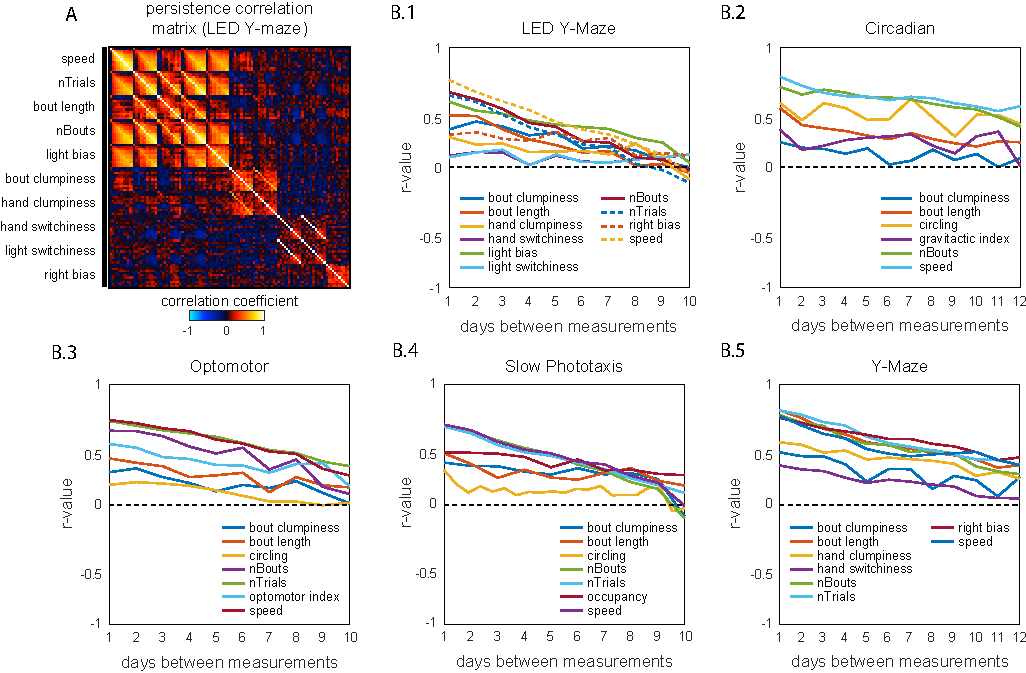
\includegraphics[width=\textwidth]{../figures/chapter_3/fig_s1.pdf}
    \vspace{.05in}
    \caption*{\textbf{Figure S1} — Persistence of primary behavioral metrics across assays. A) Example correlation matrix for 10 retests of the same individuals on a single assay (phototactic Y-Maze) across subsequent days. Rows and columns were sorted to cluster the same measures across days. B1-5)  Plots of average correlation coefficient (r-value) as a function of the days between measurements. Colors indicate the metric within each plot separately (see legends). Dashed black line denotes no correlation (r=0). Metrics in all assays showed persistent individual variation that diminished over time.}
\end{figure}
\clearpage

\begin{figure}[t!]
    \includegraphics[width=\textwidth]{../figures/chapter_3/fig_s2.pdf}
    \caption*{\textbf{Figure S2} — Genomic sequencing to confirm isogeny of BKiso. Fraction of BerlinKiso flies (n=192) that were heterozygous at any given position in the genome. Less than 10\% of flies were heterozygous at most sites. Flies showed evidence of residual heterozygosity at approximately 75 sites throughout the genome.}
\end{figure}
\clearpage

\begin{figure}[t!]
    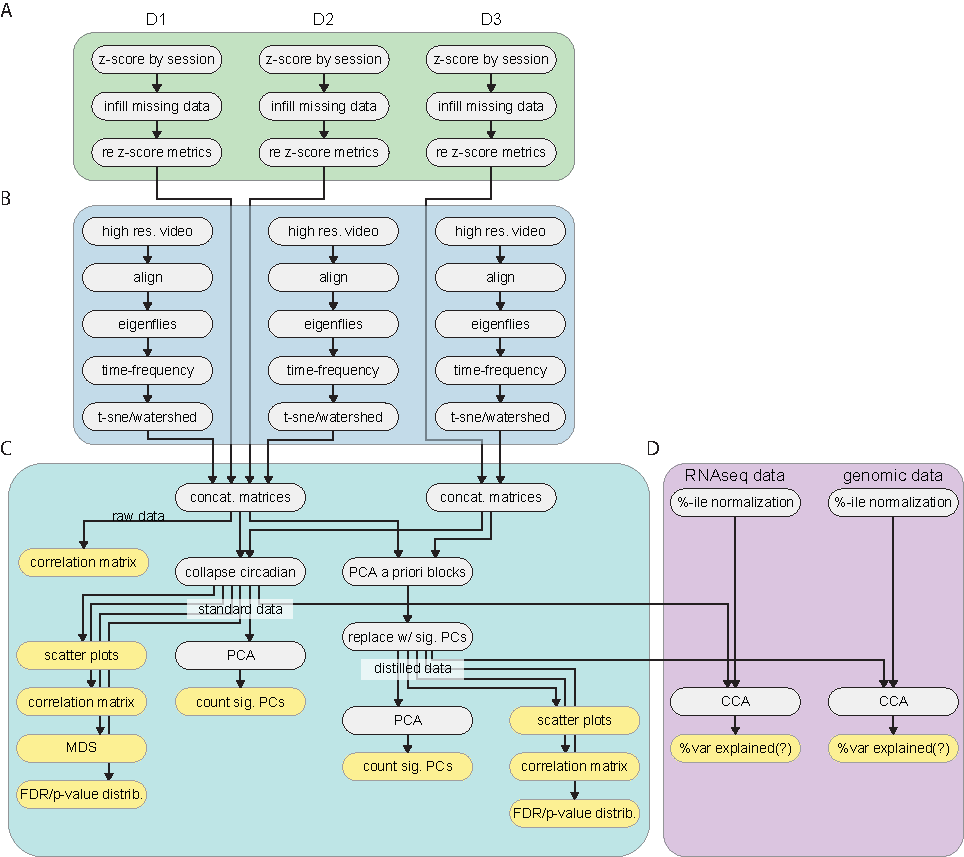
\includegraphics[width=\textwidth]{../figures/chapter_3/fig_s3.pdf}
    \caption*{\textbf{Figure S3} — Schematic of the decathlon analysis pipeline. A) Decathlon behavioral data preprocessing pipeline. Metrics are z-scored by imaging session to adjust for batch effects. Missing data is infilled with an ALS imputed matrix calculated as the average of 200 ALS imputations. B) Data acquisition and analysis for the unsupervised behavioral classification pipeline. High resolution, high frame rate single fly videos are aligned to a template fly and compressed into principal component time series (i.e. eigenflies). PC time series are then decomposed into 25 frequency spectral time series via Morlet wavelet transformation. The resulting high dimensional data is then embedded into two dimensions with t-SNE and then clustered into discrete behavioral modes via watershed transformation. C) Diagram of decathlon behavioral data analysis. Data from the decathlon assays and unsupervised behavioral classifications are combined into master behavioral data matrices for inbred (left) and outbred (right) flies separately. The covariance structure and effective dimensionality of the resulting matrices are then analyzed independently or are compressed into a “distilled” matrix with fewer dimensions. Distilled matrices are generated by retaining significant PCs within each a priori metric group above or within the variance explained by a model of n-independent dimensions (see methods). D). Individual flies undergo gene expression profiling via RNAseq. Gene expression and behavioral data are then analyzed with canonical correlation analysis to identify principal axes of gene expression that are correlated to principal axes of behavior.}
\end{figure}
\clearpage

\begin{figure}[t!]
    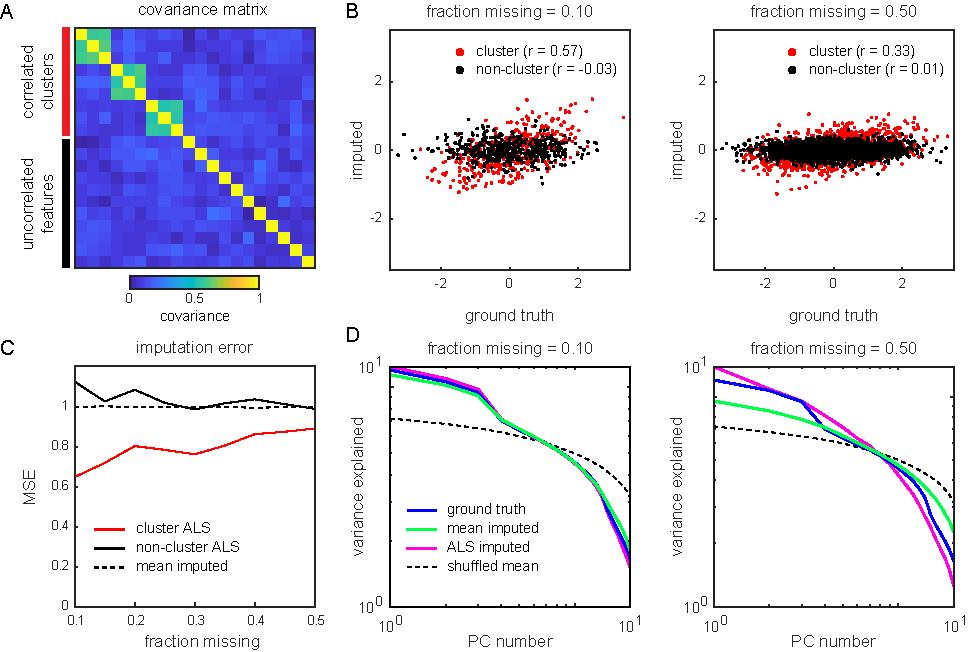
\includegraphics[width=\textwidth]{../figures/chapter_3/fig_s4.pdf}
    \vspace{.05in}
    \caption*{\textbf{Figure S4} — Toy data comparison of matrix-infilling methods. A) Covariance matrix of a toy data set generated from a multivariate normal distribution with covariance = 0.5 for features in correlated clusters (red block) and covariance = 0 for independent features. B) Scatter plots of data from a ground truth vs the same data infilled with average ALS imputation (200 repetitions) after randomly deleting either 10\% (left) and 50\% (right) of the entries. Color indicates whether the data belonged to a correlated cluster as in A. C) Comparison of mean squared error (MSE) for mean infilled and ALS average infilled data. D) Log scree plots of the variance explained for ranked principal components resulting from PCA on the ground truth, mean infilled, average ALS infilled, and shuffled matrix.}
\end{figure}
\clearpage

\begin{figure}[t!]
    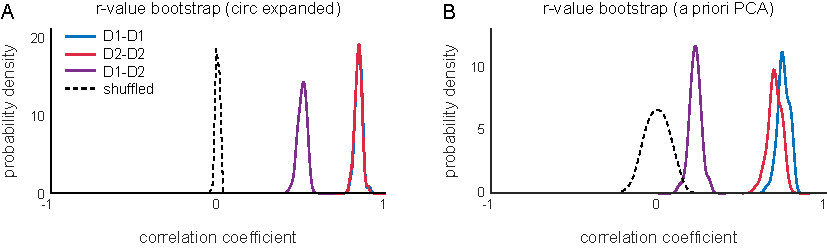
\includegraphics[width=\textwidth]{../figures/chapter_3/fig_s5.pdf}
    \vspace{.05in}
    \caption*{\textbf{Figure S5} — Correlation of correlation matrix values between D1 vs D2 and shuffled matrices. A) Distributions of correlation of full matrix correlation matrices across bootstrap replicates. Correlation coefficients were calculated by bootstrap resampling data matrices (decathlon-1 or decathlon-2) and computing the correlation matrix. Correlation was then computed between two matrices (i.e. either the same or different matrices across resamplings). B) Distributions of correlation of distilled matrix correlation matrices across bootstrap replicates as in A.}
\end{figure}
\clearpage

\begin{figure}[t!]
    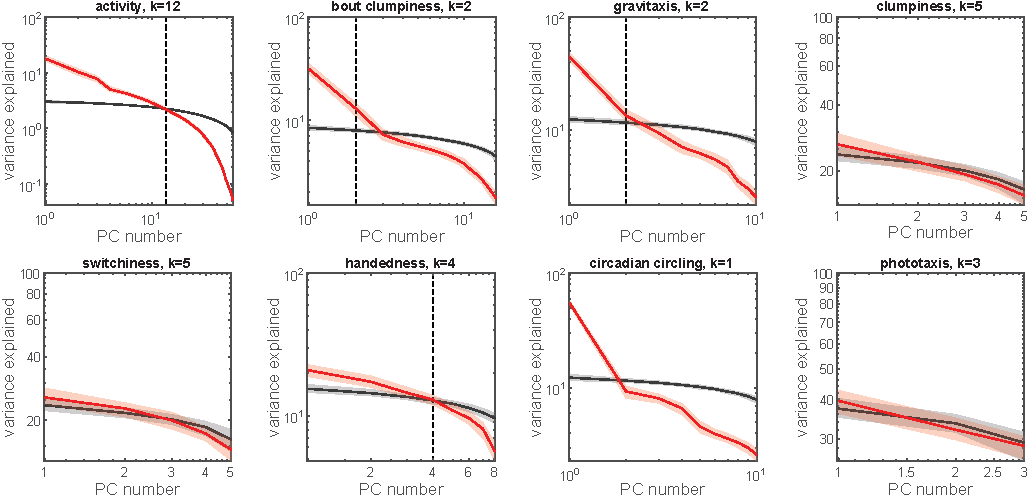
\includegraphics[width=\textwidth]{../figures/chapter_3/fig_s6-1.pdf}
    \vspace{.05in}
    \caption*{\textbf{Figure S6} — PCA of a priori groups. A) Log scree plots of the normalized ranked eigenvalues (i.e. variance explained) for PCA performed on metrics from each a priori group separately. Color indicates observed or shuffled data. Shaded regions correspond to 95\% confidence intervals as calculated by bootstrap resampling. The number of significant PCs (k) was calculated as the highest rank PC above or within the 95\% confidence interval of the shuffled matrix variance explained. B) Metric loadings of significant PCs for each a priori group (following pages).}
\end{figure}
\clearpage
\begin{figure}[t!]
    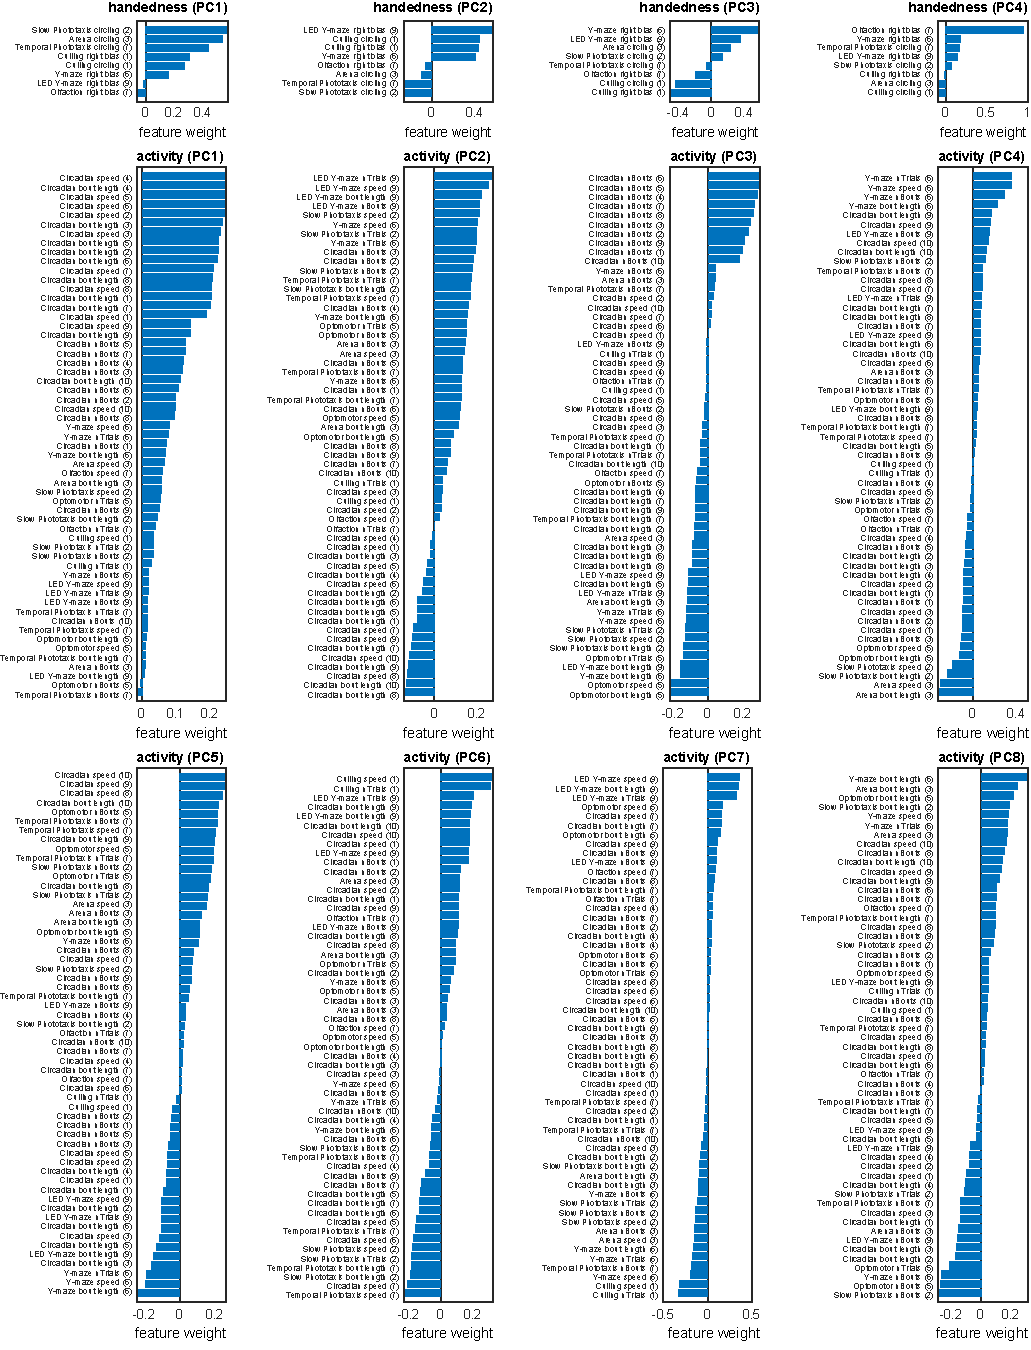
\includegraphics[width=\textwidth]{../figures/chapter_3/fig_s6-2.pdf}
\end{figure}
\clearpage
\begin{figure}[t!]
    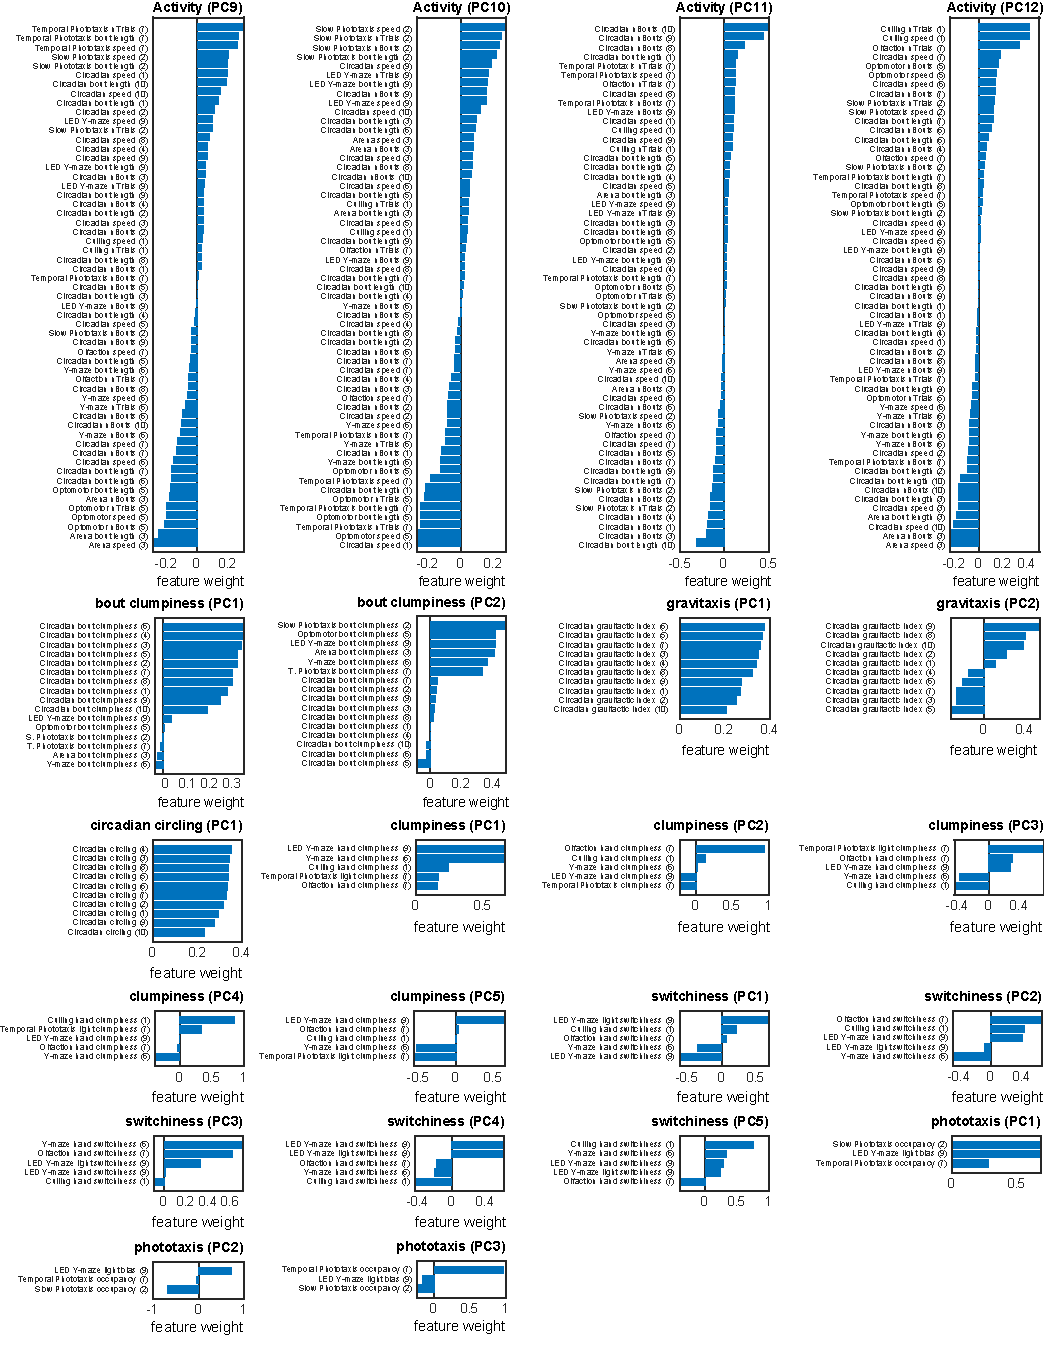
\includegraphics[width=\textwidth]{../figures/chapter_3/fig_s6-3.pdf}
\end{figure}
\clearpage

\begin{figure}[t!]
    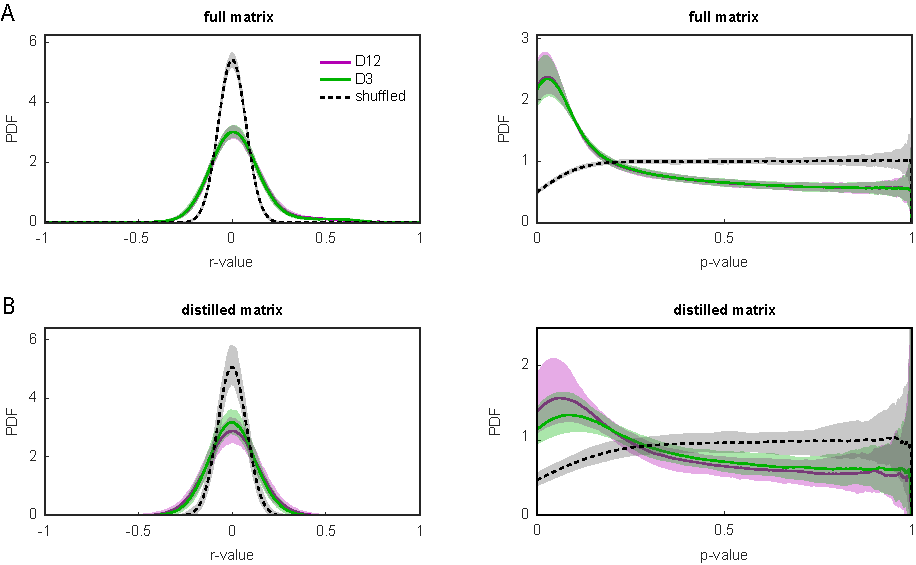
\includegraphics[width=\textwidth]{../figures/chapter_3/fig_s7.pdf}
    \vspace{.05in}
    \caption*{\textbf{Figure S7} — Distribution of correlation coefficients and p-values in the full and distilled correlation matrix. A) Kernel density estimates of the unique (i.e. lower matrix triangle) correlation coefficients in the full (top) and distilled (bottom) correlation matrices. Distributions exclude duplicates pairwise and self correlations. B) Kernel density of the the unique p-values for the correlation coefficients in A. In all plots, dashed lines indicate distributions for column-wise (i.e. within each feature) shuffled matrices. Shaded regions correspond to 95\% confidence interval calculated by bootstrap resampling.}
\end{figure}
\clearpage

\begin{figure}[t!]
    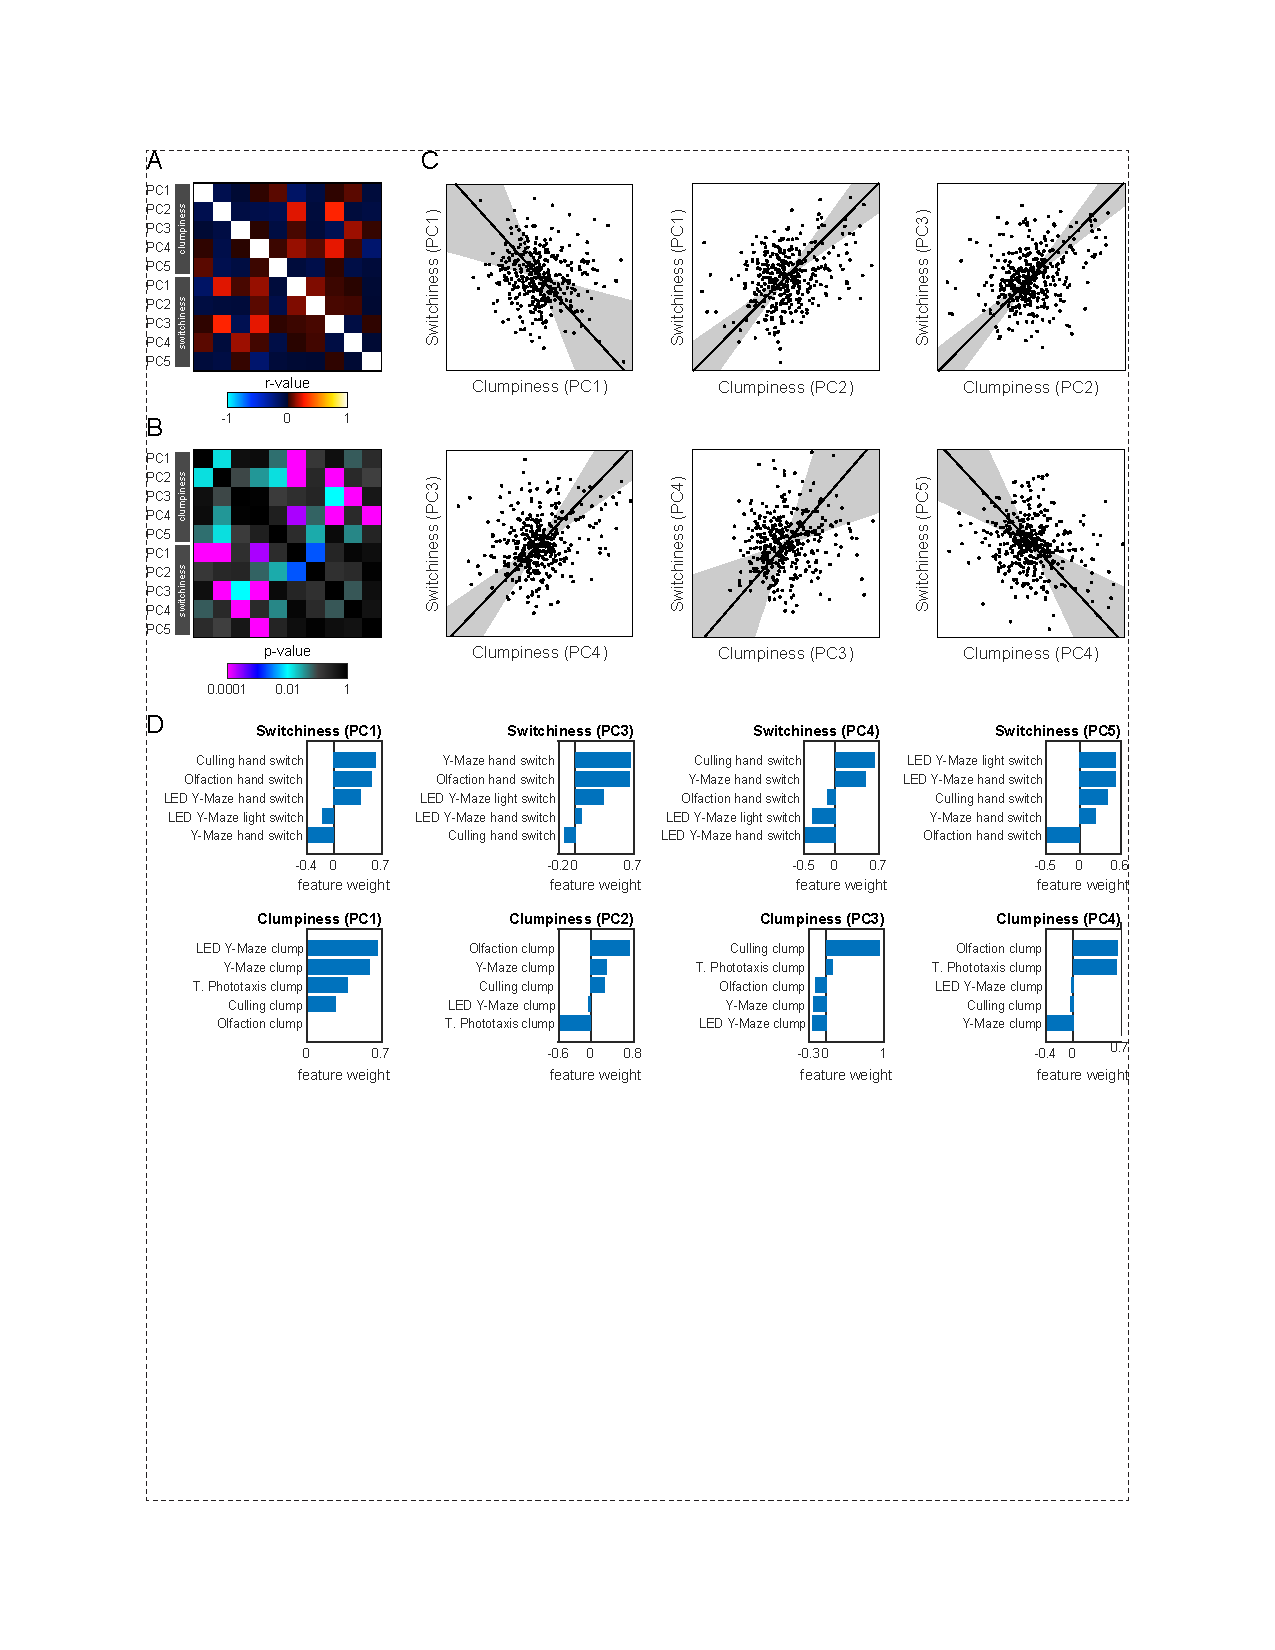
\includegraphics[width=\textwidth]{../figures/chapter_3/fig_s8.pdf}
    \vspace{.05in}
    \caption*{\textbf{Figure S8} — Significant correlations among the principal components of switchiness and clumpiness. A) Subset of the distilled correlation matrix corresponding to the significant PCs of switchiness and clumpiness. B) P-value matrix for the correlation coefficients in A. C) Scatter plots of significant correlations between switchiness and clumpiness. Points correspond to individual flies. Line indicates the line of best fit and the shaded region indicates the 95\% confidence interval of the fit as calculated by bootstrap resampling. D) Metric loadings for the PCs in C}
\end{figure}
\clearpage

\begin{figure}[t!]
    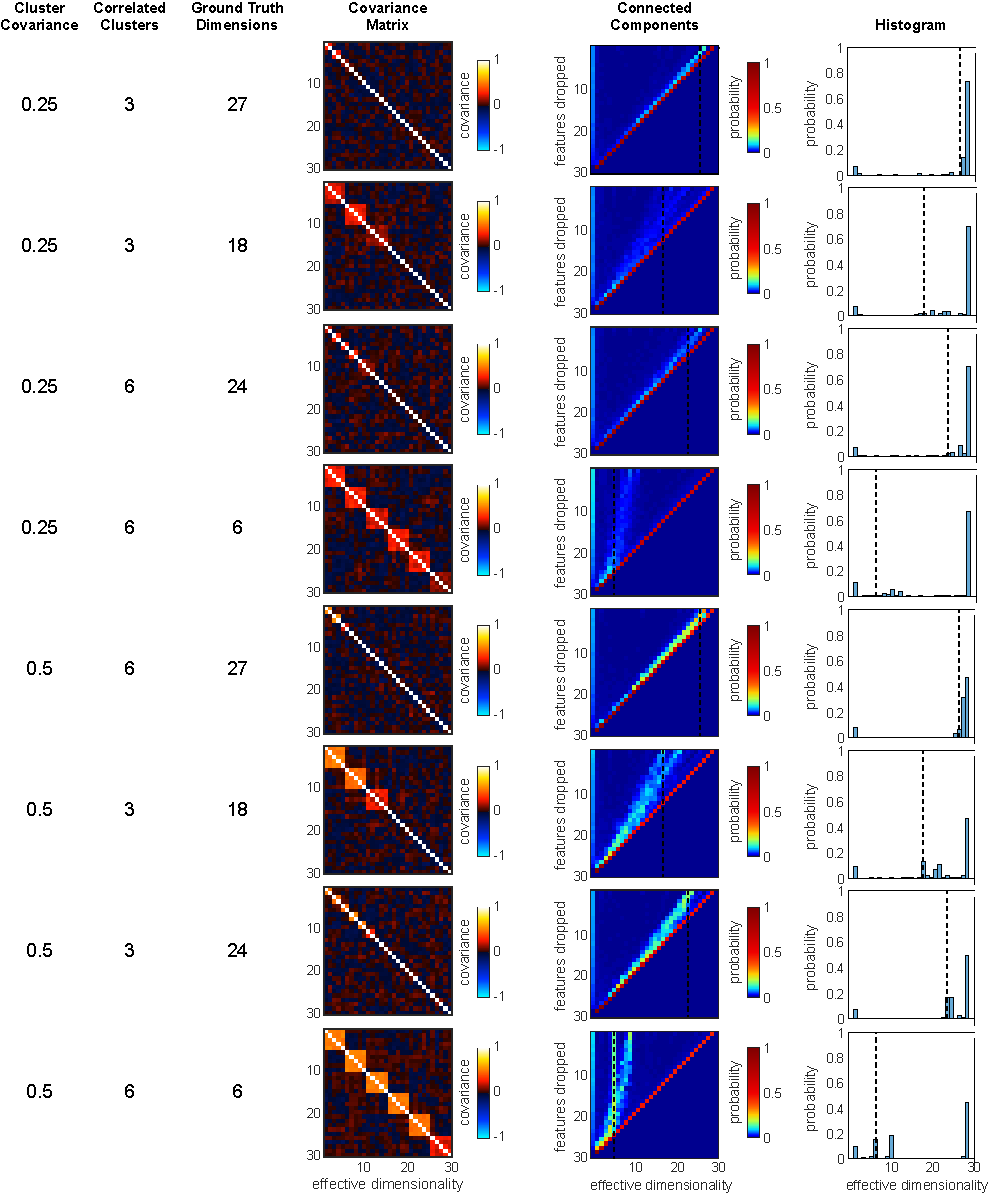
\includegraphics[width=0.85\textwidth]{../figures/chapter_3/fig_s9.pdf}
    \vspace{.05in}
    \caption*{\textbf{Figure S9} — Effective dimensionality simulations with toy data. A) Parameters used to generate a 200x30 ground truth matrix from a multivariate normal distribution as in figure S4.  Cluster covariance refers to the covariance between features belonging to the same correlated cluster. Correlated clusters corresponds to the total number of such clusters. Ground truth dimensionality is the sum of number of correlated clusters and the total number of independent features. B) Covariance matrices of toy data sets with correlated clusters along the diagonal. One cluster in each data set has covariance equal to half of the remaining clusters. C) Effective dimensions heatmap as a function of number of features retained in the toy data after dropping N random features. Rows correspond to histograms of number of connected components in the covariance matrices. D) Connected components histogram for the full covariance matrix (i.e. the top row of C).}
\end{figure}
\clearpage

\end{document}




